\documentclass[a4paper,12pt,twoside,BCOR=10mm,toc=listof]{scrbook}

% University of Iceland MSc thesis template V2.0.1 (8.4.2022),
% adapted for the current thesis materials.

\usepackage[utf8]{inputenc}
\DeclareUnicodeCharacter{2212}{\ensuremath{-}}
\DeclareUnicodeCharacter{00B0}{\ensuremath{^\circ}}
\DeclareUnicodeCharacter{00B1}{\ensuremath{\pm}}
\DeclareUnicodeCharacter{03B5}{\ensuremath{\varepsilon}}
\DeclareUnicodeCharacter{03BC}{\ensuremath{\mu}}
\DeclareUnicodeCharacter{00B3}{\ensuremath{^3}}
\usepackage[icelandic,english]{babel}
\usepackage[T1]{fontenc}
\usepackage{graphicx}
\usepackage[intoc]{nomencl}
\usepackage{enumerate}
\usepackage{xcolor}
\newcommand{\draftchange}[1]{\textcolor{red}{#1}}

% Code listings (used for RC4 routine etc.)
\usepackage{listings}
\renewcommand{\lstlistlistingname}{List of Listings}
\lstset{%
  basicstyle=\ttfamily\scriptsize,
  breaklines=true,
  columns=fullflexible
}
\renewcommand{\lstlistingname}{Code Snippet}
\renewcommand{\lstlistlistingname}{List of Code Snippets}

\usepackage{tikz}
\usetikzlibrary{positioning}
% \usetikzlibrary{external}
% \tikzexternalize[prefix=figs/]
% NOTE: TikZ externalization requires shell-escape; disabled for Overleaf compatibility.
% Better line-breaking for long URLs/DOIs (helps avoid overfull \hbox warnings)
\usepackage{xurl}
\usepackage[pdfborder={0 0 0}]{hyperref}
\usepackage{appendix}
\usepackage{eso-pic}
\usepackage{amsmath}
\usepackage{amssymb}
\usepackage{subfigure}
\usepackage[format=plain,labelformat=simple,labelsep=colon]{caption}
\usepackage{placeins}
\usepackage{tabularx}
\usepackage{longtable}
\usepackage{booktabs}
\usepackage{float}
\usepackage{array}
\usepackage{calc}
\usepackage{ragged2e}
\usepackage{lmodern}
\usepackage{fixcmex}
\usepackage{microtype}
\usepackage{needspace}
\usepackage{rotating}
% Give TeX a little extra flexibility before it declares an overfull line
\setlength{\emergencystretch}{2em}

\graphicspath{{figs/}}

\usepackage[style=numeric,sorting=none]{biblatex}
\usepackage{csquotes}
\addbibresource{references.bib}

% HÍ blue used by the supplied template/banner.
\convertcolorspec{RGB}{16,9,159}{rgb}\tmphiblue
\definecolor{hiblue}{rgb}{\tmphiblue}

% Visible reminders for unfinished thesis details during editing.
\newcommand{\thesisnote}[2]{\textcolor{red}{\textbf{#1:} #2}}

\setlength{\parskip}{\baselineskip}
\setlength{\parindent}{0cm}
\raggedbottom
\clubpenalty=10000
\widowpenalty=10000
\displaywidowpenalty=10000
\setcounter{topnumber}{3}
\setcounter{bottomnumber}{2}
\setcounter{totalnumber}{5}
\renewcommand{\topfraction}{0.85}
\renewcommand{\bottomfraction}{0.70}
\renewcommand{\textfraction}{0.10}
\renewcommand{\floatpagefraction}{0.75}
\AddToHook{cmd/section/before}{\Needspace{5\baselineskip}}
\AddToHook{cmd/subsection/before}{\Needspace{4\baselineskip}}
\AddToHook{cmd/subsubsection/before}{\Needspace{3\baselineskip}}
\setkomafont{captionlabel}{\itshape}
\setkomafont{caption}{\itshape}
\setkomafont{section}{\FloatBarrier\Large}
\setcapwidth{\textwidth}
\setcapindent{1em}
\setcounter{secnumdepth}{2}

% ===== Thesis metadata =====
\def\thesisyear{\draftchange{2027}}
\def\thesismonth{\draftchange{February}}
\def\thesisauthor{Jezreel V. Tan}
\def\thesistitle{Design and Implementation of a Low-Power LoRa Wireless Sensor Mesh Network with Cloud Storage for Monitoring Soil Conditions on Icelandic Turf Roofs}
\def\thesissubtitle{}
\def\thesisshorttitle{Low-Power LoRa Mesh Network for Icelandic Turf Roofs}
\def\thesiscredits{60}
\def\thesissubject{Electrical and Computer Engineering}
\def\thesiskind{M.Sc.}
\def\thesiskindformal{Magister Scientiarum}
\def\thesisschool{School of Engineering and Natural Sciences}
\def\thesisfaculty{Electrical and Computer Engineering}
\def\thesisaddress{Dunhagi 5}
\def\thesispostalcode{107}
\def\thesistelephone{525 4000}
\def\thesissupervisors{Helgi Þorbergsson, Ph.D.\\
Dórótea Höeg Sigurðardóttir}
\def\thesisnrofsupervisors{1}
\def\thesiscommittee{}
\def\thesisexaminer{}
\def\thesisISBN{}
\def\thesisprinting{}
\def\thesislicense{This thesis may not be copied in any form without the author's permission.}
\newcommand{\removelinebreaks}[1]{\begingroup\def\\{}#1\endgroup}

\begin{document}
\hypersetup{pageanchor=false}
\pagenumbering{arabic}

\begin{titlepage}
  \thispagestyle{empty}
  \begin{tikzpicture}[remember picture,overlay]
    \node[anchor=north west, inner sep=0pt] at (current page.north west)
        {
\includegraphics[width=\paperwidth]{banner.png}};
    \node(bottom)[shape=rectangle, fill=hiblue, minimum height=10mm, minimum width=\paperwidth, anchor=south west] at (current page.south west) {};
    \node[above=0.4cm of bottom] {
      \begin{tabular}{c}
        \sffamily \small \textcolor{hiblue}{\textbf{\MakeUppercase{Faculty of \thesisfaculty{}}}}
      \end{tabular}
    };
  \end{tikzpicture}

  \enlargethispage{3cm}
  \vspace*{3.5cm}
  \newlength{\currentparskip}
  \setlength{\currentparskip}{\parskip}
  % Center the title block without pushing it beyond the text area (prevents overfull \hbox)
  \noindent\begin{minipage}[t][20.0cm]{\textwidth}
    \setlength{\parskip}{\currentparskip}
    \begin{center}
      \vspace*{\stretch{1.5}}
      \begin{minipage}{0.95\linewidth}
        \centering
        \LARGE \sffamily \bfseries \thesistitle{}
      \end{minipage}
      \par
      \normalfont \LARGE \sffamily \thesissubtitle{}
      \vspace{\stretch{1.2}}
      \normalfont \Large \sffamily \thesisauthor{}\par
      \vspace*{\stretch{2.75}}
      \thesismonth{}~\thesisyear{}
      \vspace{\stretch{0.5}}
      \normalfont \Large \sffamily {\thesiskind{}~thesis \\
      in \thesissubject{}}
      \vspace*{\stretch{1.0}}
    \end{center}
  \end{minipage}

  % Start the next title-page block on a fresh page.
  % Insert an intentionally blank page after the cover.
  \newpage
  \thispagestyle{empty}\mbox{}
  \newpage
  \thispagestyle{empty}
  \begin{center}
    \vspace*{\stretch{0.5}}
    \Large \sffamily \bfseries \thesistitle{}
    \normalfont \large \sffamily \thesissubtitle{}\\
    \vspace*{\stretch{1.0}}
    \sffamily{\thesisauthor{}}\\
    \vspace*{\stretch{1.0}}
    \normalsize \thesiscredits{}~ECTS thesis submitted in partial fulfillment of a \\
    \textit{\thesiskindformal{}} degree in \thesissubject{}\\
    \large
    \ifx\thesissupervisors\empty\else
      \vspace*{\stretch{1.0}}
      \draftchange{Supervisors} \\
      \thesissupervisors{} \\
    \fi
    \vspace*{\stretch{1.0}}
    Faculty of \thesisfaculty \\
    \thesisschool \\
    University of Iceland \\
    \draftchange{Reykjavík}, \thesismonth~\thesisyear
    \vspace*{\stretch{0.5}}
  \end{center}

  \newpage
  \thispagestyle{empty}
  \vspace*{\fill}
  \sffamily{\removelinebreaks{\thesistitle}} \\
  \ifx\thesisshorttitle\empty\else
      (\sffamily{\thesisshorttitle{}}) \\\\
  \fi
  \thesiscredits{}~ECTS thesis submitted in partial fulfillment of a
  \thesiskind{}~degree in \thesissubject{} \\\\
  Faculty of \thesisfaculty \\
  \thesisschool \\
  University of Iceland \\
  \thesisaddress \\
  \thesispostalcode, \draftchange{Reykjavík}, Iceland \\\\
  Telephone: \thesistelephone \\\\
  \vspace{\lineskip}
  Bibliographic information: \\
  \thesisauthor{} (\thesisyear{}) \emph{\removelinebreaks{\thesistitle{}}},
  \thesiskind{}~thesis, Faculty of \thesisfaculty, University of Iceland. \\\\
  Copyright \textcopyright~\thesisyear~\thesisauthor \\
  \thesislicense{} \\\\
  \draftchange{Reykjavík}, Iceland, \thesismonth~\thesisyear

  \newpage
  \thispagestyle{empty}\mbox{}
\end{titlepage}

\cleardoublepage
\pagenumbering{roman}
\setcounter{page}{5}

\chapter*{Abstract}
\addcontentsline{toc}{chapter}{Abstract}
\draftchange{This thesis presents the design, implementation, and evaluation of a low-power LoRa-based wireless sensor network for monitoring soil and environmental conditions beneath Icelandic turf roofs. The system consists of sensor nodes built around Arduino Pro Mini microcontrollers, with capacitive soil moisture sensors, DS18B20 soil temperature sensors, AHT10 air temperature and humidity sensors, local SD card storage, and 433 MHz LoRa communication. A base station forwards collected measurements to the ThingSpeak cloud platform for remote access and visualization.}

\draftchange{Laboratory and field tests were conducted to evaluate power consumption, communication performance, sensor calibration, and cloud data transmission. Under the defined operating cycle, the sensor node consumed an average current of approximately 3.08 mA. With three 3,500 mAh battery cells connected in parallel, providing a nominal capacity of 10,500 mAh, the estimated operating lifetime was approximately 142 days. This is an idealized estimate and does not account for reductions in usable battery capacity at low temperatures.}

\draftchange{Field testing in the semi-urban area of Vellir in Hafnarfj\"{o}r\dh ur demonstrated reliable single-hop LoRa communication within an approximate 3 km radius using 433 MHz antennas. Communication performance varied with antenna placement and environmental obstacles. Calibration of the capacitive soil moisture sensor produced a second-order relationship over the tested 0--40\% moisture range, with an in-sample root mean square error of approximately 3.01 percentage points against the gravimetric calibration targets.}

\draftchange{During cloud integration tests, ThingSpeak uploads took approximately 1--2 seconds on average. The system was also deployed at Keldur to monitor environmental conditions beneath four turf roofs, with first-to-last valid record spans of approximately 51 to 130 days across the four sensor nodes. The results demonstrate the feasibility of implementing a low-cost monitoring system for Icelandic turf roofs, while highlighting the need to consider environmental conditions and long-term hardware reliability.}

\vfill
\textbf{Keywords:} wireless sensor network (WSN), LoRa, mesh network, soil moisture, turf roofs, environmental monitoring, low-power systems, ThingSpeak

\chapter*{Útdráttur}
\addcontentsline{toc}{chapter}{Útdráttur}
\draftchange{Í þessari ritgerð er fjallað um hönnun, smíði og mat á orkunýtnu þráðlausu skynjaraneti sem byggir á LoRa-fjarskiptum og er ætlað til að fylgjast með jarðvegs- og umhverfisaðstæðum undir íslenskum torfþökum. Kerfið samanstendur af skynjaraeiningum sem byggja á Arduino Pro Mini-stýrieiningum, með rýmdarmælum fyrir jarðvegsraka, DS18B20-hitanemum fyrir jarðvegshita, AHT10-nemum fyrir lofthita og rakastig, staðbundinni gagnageymslu á SD-korti og 433 MHz LoRa-fjarskiptum. Móttökustöð sendir mælingarnar áfram til ThingSpeak-skýjaþjónustunnar, þar sem hægt er að nálgast og skoða gögnin.}

\draftchange{Rannsóknarstofuprófanir og prófanir við raunverulegar aðstæður voru framkvæmdar til að meta orkunotkun, fjarskiptaafköst, kvörðun skynjara og gagnaupphleðslu í skýið. Við skilgreindan rekstrarferil var meðalstraumnotkun skynjaraeiningar um 3,08 mA. Með þremur 3.500 mAh rafhlöðufrumum tengdum samhliða, með samtals uppgefinni afkastagetu upp á 10.500 mAh, var áætlaður rekstrartími um 142 dagar. Þetta er fræðilegt mat sem tekur ekki tillit til minnkunar á nýtanlegri rafhlöðugetu við lágt hitastig.}

\draftchange{Við prófanir í hálfþéttbýlu umhverfi í Völlum í Hafnarfirði náðust áreiðanleg LoRa-fjarskipti yfir eina tengingu innan um 3 km radíuss með 433 MHz loftnetum. Afköst fjarskiptanna voru háð staðsetningu loftneta og hindrunum í umhverfinu. Við kvörðun rýmdarmælis fyrir jarðvegsraka fékkst annars stigs samband á prófuðu rakabili, 0--40\%, með um það bil 3,01 prósentustiga kvaðratrótarmeðalskekkju (RMSE) miðað við þyngdarmælingar á sömu kvörðunargögnum.}

\draftchange{Upphleðslur gagna til ThingSpeak tóku að meðaltali um 1--2 sekúndur. Kerfið var einnig sett upp á Keldum til að fylgjast með umhverfisaðstæðum undir fjórum torfþökum, og spönnuðu gildar mælingar frá fyrstu til síðustu skráningu um það bil 51 til 130 daga eftir skynjaraeiningum. Niðurstöðurnar sýna að raunhæft er að þróa ódýrt vöktunarkerfi fyrir íslensk torfþök, en jafnframt þarf að taka mið af umhverfisaðstæðum og áreiðanleika vélbúnaðar til lengri tíma.}

\vfill
\draftchange{\textbf{Lykilorð:} þráðlaust skynjaranet, LoRa, möskvakerfi, jarðvegsraki, torfþök, umhverfisvöktun, orkunýting, ThingSpeak}

\chapter*{Acknowledgements}
\addcontentsline{toc}{chapter}{Acknowledgements}

\draftchange{I would like to thank God for the opportunities, experiences, and life I have been given.}

\draftchange{I am grateful to my Icelandic and Filipino families for supporting me throughout my studies and for welcoming me into their homes while I settled into life in Iceland.}

\draftchange{I would like to thank my thesis supervisors for their guidance and feedback, as well as the staff of the University of Iceland and the National Museum of Iceland for their assistance and cooperation.}

\draftchange{I would also like to thank my friends for their support and companionship throughout my studies.}

\draftchange{Finally, I would like to thank Össur for providing me with the opportunity to work while completing my studies, as well as the tools, knowledge, and experience that contributed to this thesis.}

\chapter*{About the Author}
\addcontentsline{toc}{chapter}{About the Author}

\draftchange{Jezreel Tan is a master's student at the University of Iceland with a long-standing interest in firmware and embedded systems. His interest in firmware began at a young age and developed into a professional career as a firmware engineer prior to pursuing his master's degree. His technical interests include embedded systems, electronics, wireless communication, and Internet of Things technologies.}

\draftchange{Alongside his studies, Jezreel works at Össur, where he has gained further practical experience and technical knowledge. His master's thesis focuses on the design and implementation of a low-power LoRa-based wireless sensor network for monitoring environmental conditions beneath Icelandic turf roofs.}

\draftchange{Outside of technology, Jezreel is a self-described nerd with a strong interest in extreme sports. He enjoys enduro mountain biking and snowboarding, which have occasionally competed with his thesis for his attention and, admittedly, contributed to a few delays along the way.}

\chapter*{Abbreviations}
\addcontentsline{toc}{chapter}{Abbreviations}
\begingroup
\small
\color{purple}
\begin{longtable}{@{}p{0.18\textwidth}p{0.76\textwidth}@{}}
ADC & Analog-to-Digital Converter\\
ADR & Adaptive Data Rate\\
AES & Advanced Encryption Standard\\
AH & Absolute Humidity\\
API & Application Programming Interface\\
AWS & Amazon Web Services\\
BW & Bandwidth\\
CR & Coding Rate\\
CRC & Cyclic Redundancy Check\\
CSMA/CA & Carrier Sense Multiple Access with Collision Avoidance\\
ECTS & European Credit Transfer and Accumulation System\\
FDR & Frequency Domain Reflectometry\\
FPGA & Field-Programmable Gate Array\\
GCP & Google Cloud Platform\\
GPIO & General-Purpose Input/Output\\
GSM & Global System for Mobile Communications\\
HTTP & Hypertext Transfer Protocol\\
I²C & Inter-Integrated Circuit\\
ID & Identifier\\
IDE & Integrated Development Environment\\
IPv6 & Internet Protocol version 6\\
ISM & Industrial, Scientific, and Medical\\
IoT & Internet of Things\\
LED & Light-Emitting Diode\\
Li-Ion & Lithium-Ion\\
LoRa & Long Range\\
LPWAN & Low-Power Wide-Area Network\\
MCU & Microcontroller Unit\\
MOSFET & Metal-Oxide-Semiconductor Field-Effect Transistor\\
NB-IoT & Narrowband Internet of Things\\
NTP & Network Time Protocol\\
OOP & Object-Oriented Programming\\
PCB & Printed Circuit Board\\
PL & Payload Length\\
RC4 & Rivest Cipher 4\\
RF & Radio Frequency\\
RH & Relative Humidity\\
RMSE & Root Mean Square Error\\
RSSI & Received Signal Strength Indicator\\
RTC & Real-Time Clock\\
RX & Receive\\
SaaS & Software as a Service\\
SD & Secure Digital\\
SF & Spreading Factor\\
SNR & Signal-to-Noise Ratio\\
SoC & System on Chip\\
SPI & Serial Peripheral Interface\\
TDR & Time Domain Reflectometry\\
TP & Transmission Power\\
TX & Transmit\\
UAV & Unmanned Aerial Vehicle\\
USB & Universal Serial Bus\\
VWC & Volumetric Water Content\\
WBAN & Wireless Body Area Network\\
Wi-Fi & Wireless networking technology\\
WSN & Wireless Sensor Network\\
\end{longtable}
\endgroup
\hypersetup{pageanchor=true}
\tableofcontents
\listoffigures
\listoftables
\lstlistoflistings


% Start main matter page numbering at the Introduction
\cleardoublepage
\pagenumbering{arabic}
\setcounter{page}{1}
\chapter{Introduction}
\section{Definition of Terms}
\subsection{Turf House}

A turf house is defined as a structure or building whose roof and walls
are mainly made from turf. Sometimes, these can be mixed with gravel or
stones for extra support. Timber beams and rafters are used as the main
structure of the building and are also used to support and hold the
roof. Turf is also used as a main component to cover the roof, and
slates are used as an underlay. Throughout the years, the material used
for turf houses has not changed drastically, but the form of these
houses has changed and adapted through the ages \cite{ref14}\cite{ref15}.

\subsection{Soil Moisture}

Soil moisture is defined as the amount or quantity of water in the soil
\cite{ref16}\cite{ref17}. It can be further defined as the amount of water held
in between the pores of the soil. These volumes of water may be in
liquid or vaporized form \cite{ref18}. When measuring the amount of water in
a known amount of soil, soil moisture can be expressed as ``\% water by
weight or volume of soil'', or ``inches of water per foot of soil''
\cite{ref19}.

\subsection{Relative Humidity in Soil}

Humidity is defined as the amount of gaseous water or water vapor in the
air. High humidity means there is a lot of moisture in the air and low
humidity indicates dry conditions. Humidity is often described as
absolute humidity (AH) or relative humidity (RH) \cite{ref20}\cite{ref21}.
Absolute humidity is measured in units of g/m\textsuperscript{3} where
it is the measure of water vapor content in air that is not dependent on
temperature \cite{ref22}. Relative humidity is the ratio of the current
amount of water vapor in the air to the maximum amount the air can hold
at a given temperature, expressed as a percentage (\%) \cite{ref23}.

This study will collect data and conduct tests below the soil surface.
In this context, humidity refers to the relative humidity of the air
within the soil\textquotesingle s pores and gaps, which will be used as
data for the study.

\subsection{Wireless Sensor Network (WSN)}

A wireless sensor network (WSN) is a collection of spatially distributed
sensor nodes that measure and communicate data wirelessly using protocols
such as radio, Wi-Fi, Bluetooth, and LoRa. A sensor node may contain one
or more sensors, depending on the application, and can communicate with a
central system or with neighboring nodes in a mesh network
\cite{jung2012clusterhead,xu2014borderrouter}. WSNs are used in
environmental monitoring, industrial equipment monitoring, healthcare,
agriculture, and other distributed sensing applications. Their low-power
design makes them suitable for remote and harsh environments.

\subsection{Internet of Things (IoT)}

The Internet of Things (IoT) refers to interconnected physical devices
that collect, exchange, and process data through communication networks
and cloud services \cite{aws2024iot}. Examples include wearable devices,
tracking systems, environmental sensors, and smart infrastructure. In this
context, a WSN provides the sensing and communication layer, while the IoT
system can transmit the collected measurements to a network or cloud
platform for storage, visualization, and analysis
\cite{karthik2021iot,jebri2015iot}.

\subsection{Long Range (LoRa)}

Long Range (LoRa) is a radio-frequency modulation technology designed for
low-power wide-area network (LPWAN) applications. It supports long-range
communication with relatively low energy consumption, making it suitable
for many IoT applications and outdoor monitoring systems
\cite{dambal2019lora}. Communication range depends on factors such as
line of sight, antenna design, frequency, spreading factor, bandwidth,
transmission power, and local regulations. The sensor nodes in this study
use a 433 MHz SX1278-based LoRa module in the applicable industrial,
scientific, and medical (ISM) band. The use of 433 MHz, 868 MHz, or
915 MHz bands depends on regional regulations and deployment requirements
\cite{camarillo2022lorawan,yahya2023antenna}.

\subsection{In-Situ Sensors}

In-situ sensors measure and monitor conditions directly at the location of
interest. They provide measurements without requiring repeated manual
sampling or removal of material from the monitored environment. In-situ
sensors are useful in environmental monitoring because they can collect
data continuously from remote locations. They may include temperature,
air-quality, soil-moisture, and groundwater sensors and can be integrated
with processing and wireless communication hardware
\cite{barnhart2010groundwater}.

\subsection{Low-Power Systems}

Low-power systems are designed to operate with minimal energy consumption
over extended periods, often using batteries or harvested energy. These
systems commonly operate intermittently and use hardware and software
optimization to reduce their duty cycle. Sleep modes disable non-essential
functions while preserving the control functions needed to wake the device
at scheduled intervals. This approach is important for battery-powered IoT
devices deployed in remote areas \cite{skuta2020power, montoya2018sward}.

\subsection{Cloud-Based Data Platforms}

Cloud-based data platforms provide online infrastructure for storing,
managing, processing, and analyzing data. They allow users to access data
remotely without maintaining local high-capacity storage or computing
hardware. Cloud services are commonly used in IoT systems for device
management, data processing, visualization, and analytics. Examples include
Amazon Web Services, Google Cloud, and Microsoft Azure. In this thesis,
ThingSpeak provides the cloud-based storage and visualization service for
the collected sensor measurements \cite{sun2011cloud}.

\section{Background of the Study}
Icelandic turf houses are important cultural and architectural heritage structures whose turf construction requires continued maintenance. The literature supplied for this thesis describes the long history of turf construction in Iceland and the need to understand turf layers and their environmental conditions. Moisture is particularly relevant because turf and timber components are susceptible to deterioration, while the conservation of heritage structures requires maintenance approaches that do not unnecessarily disturb the site.

The current system design addresses this monitoring problem by placing low-power sensor nodes beneath turf roofs. The methodology specifies that nodes collect soil moisture, soil temperature, air temperature, and relative humidity, while transmitting measurements through a LoRa mesh network to a base station and cloud database. The nodes are designed to remain visually unobtrusive and to operate for extended periods with limited maintenance.

\section{Statement of the Problem}
Monitoring environmental conditions beneath turf roofs presents several engineering constraints. Sensor nodes must be sufficiently small and unobtrusive to avoid affecting the appearance of a heritage site, while also operating in an environment characterized by high moisture, freezing and thawing cycles, and possible snow coverage. The system must provide reliable wireless communication, conserve battery energy, retain measurements when transmissions are missed, and make the collected data available remotely.

The project therefore addresses the need for a practical monitoring system that combines low-cost sensing hardware, low-power operation, long-range wireless communication, local data backup, and cloud-based access in a single deployable platform.

\section{Objectives}
The study aims to design, implement, and evaluate a low-power LoRa wireless sensor mesh network for monitoring soil and environmental conditions beneath Icelandic turf roofs. The specific objectives are to:
\begin{enumerate}
\item measure soil moisture, soil temperature, air temperature, relative humidity, and battery voltage using distributed sensor nodes;
\item develop a LoRa-based mesh communication system capable of reliably transferring measurements between sensor nodes and a base station;
\item implement low-power operating modes suitable for long-duration battery-powered deployment;
\item provide local data backup so measurements are retained when wireless transmissions are missed;
\item calibrate the low-cost capacitive soil moisture sensor against reference measurements; and
\item transmit collected measurements to a cloud platform for remote access, visualization, and analysis.
\end{enumerate}

\section{Significance of the Study}
The project provides a low-cost engineering approach to continuous monitoring of environmental conditions on Icelandic turf roofs. The system is intended to support researchers and conservation personnel by providing measurements without requiring frequent manual sampling or intrusive installation. The use of off-the-shelf components and a modular mesh architecture also provides a basis for scaling the monitoring approach to additional turf-roof sites.

\section{Scope and Limitations}
The work focuses on a low-power LoRa-based wireless sensor mesh network using distributed sensor nodes and a cloud-connected base station. The implemented nodes measure soil moisture, soil temperature, air temperature, relative humidity, and battery voltage. The methodology specifies burial of sensor nodes at approximately 11 cm, weatherproof enclosures, local SD-card data backup, and a non-destructive installation approach.

The evaluation includes laboratory power-consumption testing, preliminary and intermediate field deployments around the University of Iceland, LoRa range testing around Vellir in Hafnarfjörður, long-term deployment at the Keldur turf-house site, soil moisture calibration, and ThingSpeak cloud-upload testing. The documented results also show limitations, including antenna-related packet loss during early testing, sensor-calibration issues during intermediate testing, and hardware failures affecting two nodes near the end of the long-term deployment. The calibration results cover the 0--40\% moisture range and therefore do not establish performance beyond that range.

\chapter{Review of Related Literature}
\section{Icelandic Turf Houses}

Turf houses are a significant part of culture and heritage in Iceland. A
paper published by Bathurst et al. \cite{ref01}, explains that turf has
always been widely used across regions in northern Europe for its
durability, renewability, and its abundance. It also has great
insulation properties which makes it a good choice for colder climates.
Since turf houses are unique, their appearance and construction garnered
a lot of attention and admiration from people. This leads to interesting
studies and research on their history, culture and construction
practices \cite{ref05}.

According to Lin et al. \cite{ref02}, regions such as Scotland and especially
Iceland have very limited supply of natural resources, however turf was
abundant. This made it very important for shelter construction. Turf
houses that were well built were also stated to be better in insulating
cold weather than houses built on stone and timber, which is very
important in these countries with harsh cold weather. Wunderlich et al.
\cite{ref03}, describes turf as a major component in buildings for Iceland
during the medieval period. The turf used in the construction of these
buildings was cut from local bogs or from edges of cultivated fields in
the area. For example, in Mosfellsbær, it was presumed that the bricks
of turf used were cut from the valley floor bogs, which was south of the
habitation area. The bogs were then transported to higher elevation
areas, where the difference in elevation naturally aided in draining
water, making it suitable for constructing houses \cite{ref01}.

Stone was often laid below the turf walls to prevent moisture from
seeping into the walls and eventually causing it to rot \cite{ref04}. The
amount of stone beneath the turf walls varied on use. For example, in
turf houses that sheltered animals, the stone layers were higher so that
it would prevent animals from damaging the turf by feeding on it or
rubbing against it. Archaeological studies suggest that in Iceland
specifically, the stone foundations were used less in buildings during
the Viking era when compared to later eras such as the Medieval and Post
Medieval \cite{ref03}.

Like any other natural resource with positive qualities, turf also has
its drawbacks. A book published by Nannini \cite{ref05}, explains that
insulation with turf was only tolerable since it was applied generously,
houses would have thick walls and almost completely no windows.
Additionally, settlers would burn dried manure inside these houses to
generate more heat. Combined with the lack of ventilation, this led to
very unhealthy environments. Another issue is that turf is
replenishable. This means settlers would have to renovate every few
years or so and force owners to refurbish or rebuild their home. Hannes
Larusson \cite{ref06} emphasizes this as ``an inseparable part of the turf
house'' which he later states as one of the main reasons why they were
eventually replaced by concrete.

With the innovation of concrete and the eventual abandonment of
refurbishing or maintaining these perishable turf houses, this led to
the loss and destruction of these historical buildings.

\section{Studies in Turf and Turf House
Maintenance}

Due to the unique architectural design of these turf houses, it became
one of the most researched topics on Icelandic architectural history.
Studies even dating back to the last decades of the nineteenth century
\cite{ref05}. Even today, many scholars and authors research on turf
construction from analysis of inner environment comfort to botany of the
turf layers \cite{ref07}. According to Sigurjón \cite{ref08}, many Icelandic
scholars and researchers such as architects, architectural historians
and conservation experts, have been extensively studying turf houses
solely focusing on restoring and conserving these sites.

Researchers such as Wunderlich et al. \cite{ref03}, conducted studies on
imaging medieval turf buildings in Iceland through geophysical methods.
This is to understand the structural features and subsurface
characteristics of the houses. During a study conducted by Milek and
Roberts \cite{ref09}, ash was discovered to be deposited on the floors of the
houses. This was used as insecticide and a drying material since the ash
can fill the tiny gaps and holes. It is also absorbent and hence can
protect the wooden materials from fungal decay. Studies from Milek
\cite{ref10} state that although turf buildings can last for over 100 years
when properly constructed and maintained, these buildings would still
need constant turf replacement. Specifically on the roof and walls,
since they are prone to rot. Stating that both turf and timber needs
replacement every 10 -- 20 years.

There has also been other research with goals specifically focused on
turf restoration in general. Studies conducted by Hnatowich et al.
\cite{ref11} have been transplanting healthy turf into disturbed areas with
hopes to restore it. By using native and local turf for the transplant,
there is an added benefit of lesser shock to the transplanted area.
Additionally, other studies such as those by Malleshaiah et al.
\cite{ref12}, have presented techniques such as soil aerification. This has
proved to improve turf quality by relieving the soil compaction, giving
it proper aeration and therefore improving turf quality. This is further
supported by Nunome et al. \cite{ref13} stating that soil compacting is a
major factor in the increase of degradation of turf.

With ongoing and continuous studies and discoveries on turf and turf
house construction and maintenance, preservation experts can further
study and utilize these techniques to extend the lifespan of these turf
houses. By minimizing rot and decay on these turf and wooden structures,
especially on the roof and walls, these turf houses can be properly
maintained while preserving the cultural heritage and importance of these
historical structures.

\section{LoRa Mesh Technology}

Long Range (LoRa) technology is a low-power wireless communication
technology used in applications such as traffic-light control, smart
street lighting, environmental monitoring, smart waste management,
energy management, and the Internet of Things (IoT)
\cite{tome2018longrange,enriko2023lorawan,zhu2019mesh,lozano2018smartwaste,andrade2019lora,andrade2023smartmeter}. Its long communication range and low
power consumption make it suitable for distributed monitoring systems.
Depending on the antenna, radio configuration, terrain, and deployment
environment, LoRa communication can reach several kilometres
\cite{centenaro2016longrange}. LoRa is therefore a suitable candidate for
low-bandwidth applications that require low cost and scalability
\cite{rahman2018lora}. Its potential has also been demonstrated in IoT
applications \cite{ayele2017lora}.

\begin{figure}[htbp]
\centering
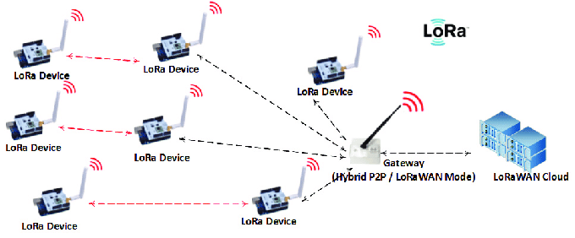
\includegraphics[width=0.8\textwidth]{figs/rrl-image1.png}
\caption{LoRa mesh technology illustrating multi-hop communication.}
\label{fig:rrl-image1}
\end{figure}

Multi-hop communication, mesh networking, and routing protocols can
extend the coverage and improve the signal reliability of LoRa networks
\cite{solar2022monitoring,sole2022mesh}. Mullick et al. reported improved
network performance when a mesh strategy was used for air-quality
monitoring, particularly under adverse environmental conditions
\cite{mullick2022mesh}. Andersen et al. also demonstrated that a LoRa mesh
network could approximately double the operating range of an asset-tracking
prototype through multi-hop communication and routing
\cite{andersen2020mesh}.

Multi-hop communication also introduces trade-offs. Although additional
hops can increase coverage, they may increase latency because nodes need
to coordinate transmissions and avoid collisions
\cite{centelles2021multihop}. This trade-off depends on the application:
some systems prioritize low latency, whereas remote environmental
monitoring systems may prioritize range, reliability, and low power
consumption. In addition, relay nodes can reduce the transmission distance
to the next node and may therefore improve energy efficiency
\cite{khonrang2022multihop}.

Compared with other low-power wireless technologies, LoRa is particularly
well suited to outdoor applications that require long range and low power.
Zigbee generally provides shorter-range communication, while NB-IoT can
provide broader cellular coverage and higher data rates at the cost of
greater dependence on cellular infrastructure and power consumption
\cite{liu2023zigbee,danladi2022lpwan}. The approximate ranges in
Table~\ref{tab:wireless-range-comparison} are indicative only and depend
strongly on the deployment environment and network configuration.

\begin{table}[htbp]
\centering
\caption{Approximate communication ranges of selected wireless technologies.}
\label{tab:wireless-range-comparison}
\begin{tabular}{lll}
\toprule
\textbf{Technology} & \textbf{Approximate range} & \textbf{Main dependency} \\
\midrule
Zigbee & 10--300 m & Local radio environment \\
LoRa & 2--15 km & Antenna, terrain, and radio settings \\
NB-IoT & Up to 100 km & Cellular network coverage \\
\bottomrule
\end{tabular}
\end{table}

\section{Low-Power Technology}

Wireless sensor networks require a reliable energy source for sensing,
processing, storage, and communication. Although some systems are powered
continuously from an outlet, remote monitoring nodes commonly rely on
batteries. For long-term deployments, reducing energy consumption is
essential because battery replacement may be difficult or disruptive.
Low-power design techniques can improve energy efficiency and extend the
operational lifetime of sensor nodes \cite{lahiri2002battery}.

One common technique is to place the device in a sleep state when it is
not actively sensing or communicating. During low-power operation, most
functions are disabled while a small control subsystem remains active to
restore normal operation when required \cite{zhang2023sleep}. For systems
with low duty cycles, the sleep period is often more important to overall
energy consumption than the active period \cite{hwang2012poweraware}.

Previous studies demonstrate the practical benefits of this approach.
Kombo et al. reduced the duty cycle of a low-power monitoring system to
less than one percent, while Hung et al. reported power-consumption
reductions of approximately 38.46--54.44\% using a low-power wireless
sensor protocol \cite{kombo2021groundwater,hung2020lowpower}. These results
support the use of scheduled sensing, selective peripheral activation, and
communication sleep modes in remote environmental monitoring.

Low-power operation is therefore central to the present system. The
proposed sensor nodes periodically wake, collect measurements, transmit or
store the data, and return to a sleep state. This duty-cycle strategy
reduces average current consumption while allowing the system to continue
monitoring environmental conditions over an extended deployment period.

\section{Cloud-Based Data Visualization and Management in Research}

Cloud-based data systems provide a convenient way to store, visualize, and
manage measurements collected by remote sensor networks. Researchers can
access time-series data without physically retrieving the sensor nodes,
which is particularly useful when monitoring sites are distant or difficult
to access. Cloud platforms also provide scalable infrastructure for storing
and processing large datasets \cite{naik2017cloud,sheffield2022cloud}.

Common cloud platforms include Amazon Web Services (AWS), Google Cloud
Platform (GCP), and Microsoft Azure. These platforms support different
combinations of data storage, analytics, visualization, and Internet of
Things services \cite{aws2023,gcp2023,azure2023}. The appropriate platform
depends on the required storage capacity, processing capability, cost,
connectivity, and ease of integration with the embedded system.

For environmental monitoring, cloud-based visualization can improve the
interpretation of long-term measurements by making trends and anomalies
available remotely. In the present project, cloud connectivity is used to
upload sensor measurements to ThingSpeak, where the data can be stored and
visualized for subsequent analysis.

\section{Measuring Soil Moisture}

Measuring soil moisture is one of the fundamental techniques when
studying soil conditions in environmental monitoring research. Over the
years, soil monitoring techniques have been continuously improved, and
new methods have been developed. However, these methods vary in their
principles and specific applications.

The standard method of measuring soil moisture is the Gravimetric
Method. To measure the soil moisture, researchers must get the
difference of the natural weight of soil to the same amount of soil but
dried. This is often achieved by placing the soil in an oven to remove
moisture \cite{ref24}. Starr and Paltineanu \cite{ref25} state this method as
very simple and highly accurate to such a degree that it is often used
as a calibration for other sensors or methods. It is even used to
validate data gathered from different studies \cite{ref26}\cite{ref27}. The
formula for calculating the soil moisture is defined by:

\begin{equation}
Soil\ Moisture\ Content\ (\%) = \frac{Weight\ of\ Wet\ Soil - Weight\ of\ Dry\ Soil}{Weight\ of\ Dry\ Soil}\ x\ 100
\label{eq:gravimetric-soil-moisture}
\end{equation}

However, this method has its downsides, although being very simple. It
is very time-consuming and destructive for the study area since it
involves unearthing soil and taking the time to dehydrate it in the
oven. This makes it unsuitable for long term studies and real time
monitoring \cite{ref24}.

New and modern techniques that are highly accurate, fast and
non-destructive are the Time Domain Reflectometry (TDR) and the
Frequency Domain Reflectometry (FDR). Because there is a significant
difference between the dielectric constants of dry soil and pure water,
modern tools can easily distinguish between the two \cite{ref28}. TDR works
by placing steel rods into the soil and then sending electrical signals
through them. The signal travels from one probe through the other by
traveling through the soil. The property of wet soil makes it return the
signal slower compared to dry soil. In turn, this helps the device
determine the humidity of the soil accurately \cite{ref19}\cite{ref29}.

FDR works similarly to TDR, but instead of measuring the time it takes
for the signal to move through the soil, FDR measures the frequency of
the electromagnetic waves when it travels \cite{ref28}. When the
electromagnetic waves travel through the soil, the frequency of the
signal changes based on the moisture. This helps researchers determine
the soil moisture accurately and precisely \cite{ref30}. Although these
methods are quick and accurate without having the need to be
destructive, devices like these are expensive and can cost up to
hundreds or even thousands of dollars based on the application \cite{ref19}.

Nowadays, there are newer types of sensors which can be used to measure
soil moisture without having the need to be expensive all while being
fairly accurate, quick, and non-destructive. These sensors include
resistance-based and capacitance-based types. Resistance-based sensors
measure soil moisture by placing probes into the soil, similar to the
methods mentioned earlier. However, instead of sending electrical
signals or waves, this method measures the soil\textquotesingle s
resistance. The resistance of the soil lowers when it has a high amount
of moisture and rises when it is dry \cite{ref31}\cite{ref32}. However, Koyunco
et al. \cite{ref28} states that this method is highly unreliable because
soil types can vary in resistance which leads to imprecise results.
Additionally, the probes are prone to corrosion which can lead to no
results at all.

Capacitive sensors work by measuring the capacitance across the sensor
electrode due to humidity when deploying a pulse voltage
\cite{ref33}\cite{ref34}. González-Turel et al. \cite{ref35} explain that because
the dielectric constant of water is higher than that of air or dry soil,
the moisture content affects the dielectric constant. This results in an
increase when the soil is wet, leading to a higher capacitance that can
be detected by the sensor. Researchers like Kulmány et al. \cite{ref36}
prefer these types of sensors because they provide accurate data while
being inexpensive and easy to install. Additionally, these sensors are
less prone to oxidation and damage because they do not require exposed
probes to touch the soil; their sealed design provides adequate
protection.

Among most methods and sensors used for determining soil moisture,
typically capacitive sensors are often preferred for their accuracy,
inexpensive price, and ease of installation while being able to provide
real time data. Each method, however, has its own strength and
limitations, which are considered during research making one more
suitable than the others, especially for specific conditions.
Ultimately, the choice of sensor and methods will depend on the specific
requirements and parameters in the study and the choice of the
researchers. It's important to evaluate these factors and select the one
that is most appropriate for the study.

\chapter{Methodology}
\section{Overview}

This chapter describes the system design and presents the methodology
used to design and develop the project while achieving the objectives of
the study. It outlines the complete workflow of the project, starting
from the system concept and design requirements, through hardware and
firmware development, PCB design and manufacturing, and finally to
system deployment. The chapter also describes the calibration and
validation of the selected soil moisture sensor in comparison with
professional-class sensors.

\section{System Concept and Design
Requirements}

\subsection{System Concept}

The system is designed as a wireless mesh network using LoRa as the core
communication technology. Weatherproof wireless sensor nodes collect
data such as soil moisture, soil temperature, air humidity, and air
temperature, and transmit this data efficiently between neighboring
nodes until it reaches a base station with access to a cloud database.
The collected data is then made accessible to researchers from anywhere.

\begin{figure}[htbp]
\centering
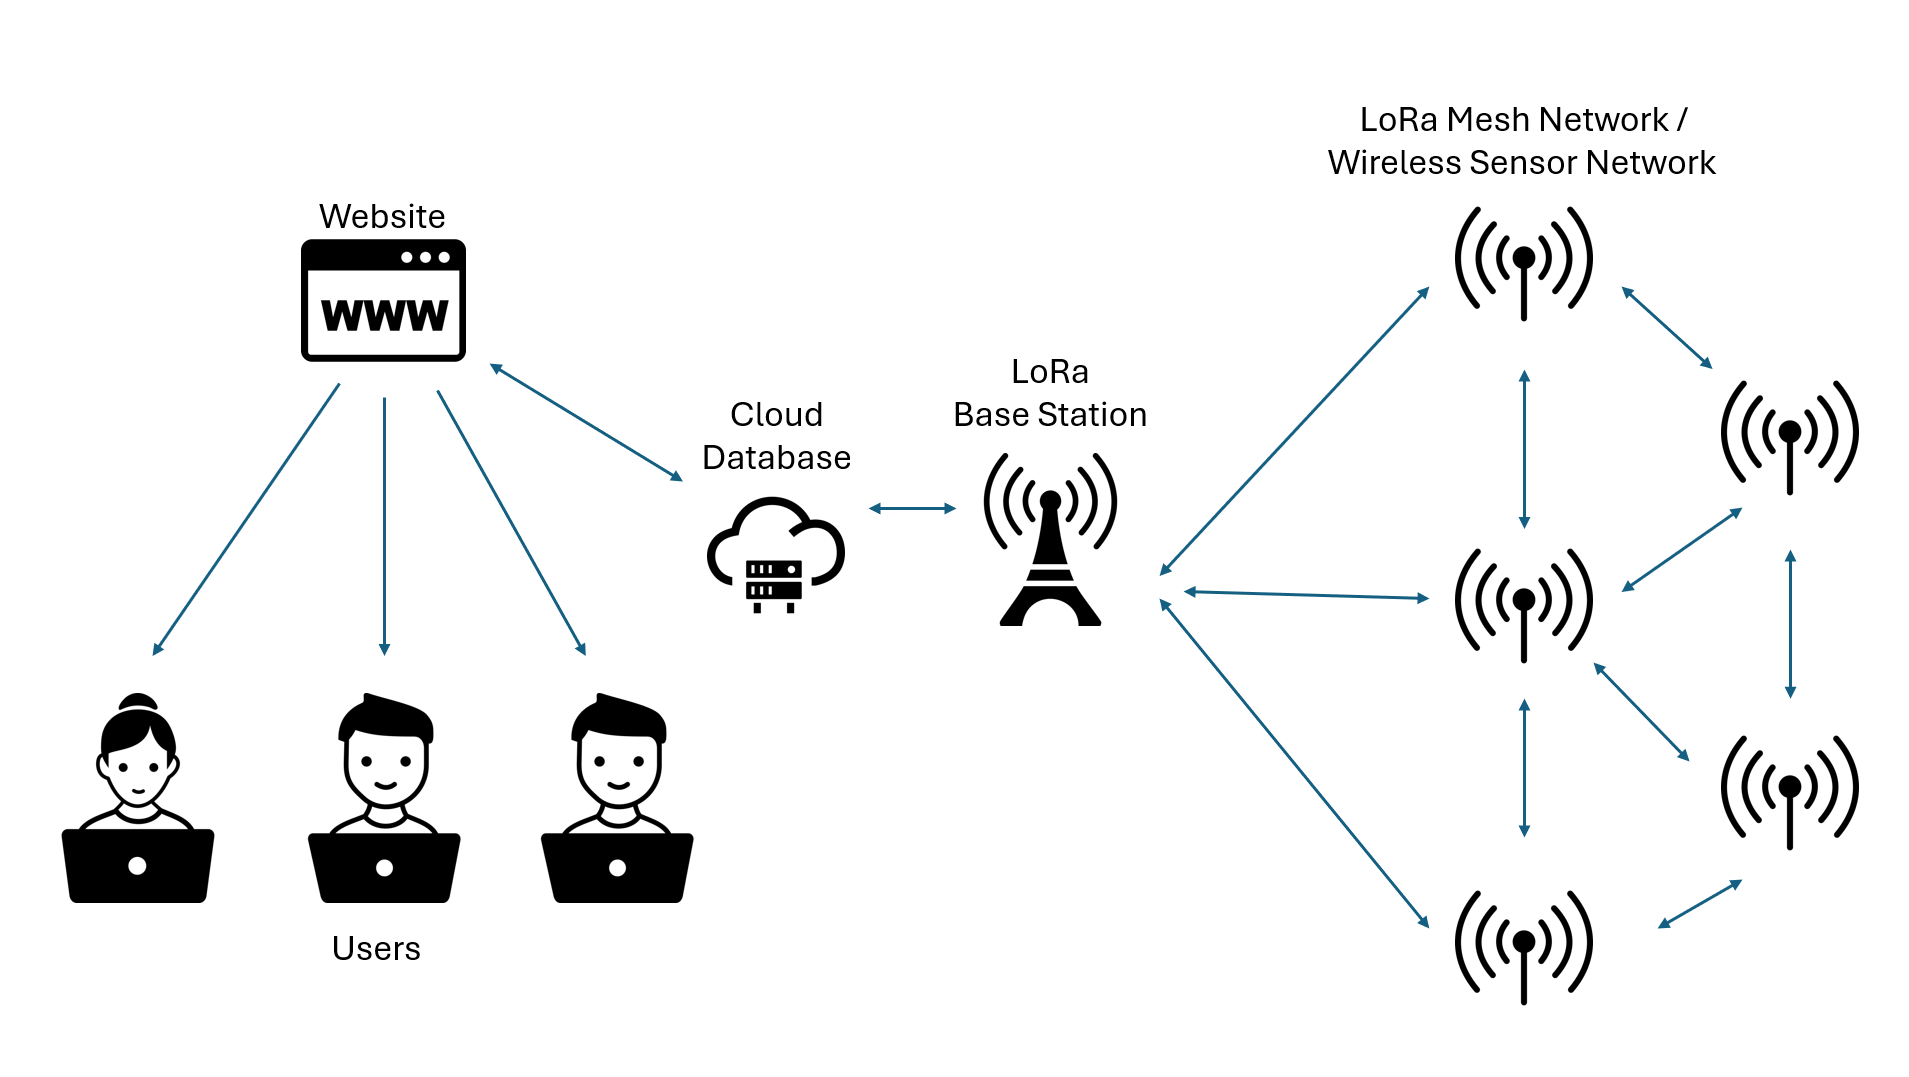
\includegraphics[width=5.03874in,height=2.8429in]{figs/method-image1.png}
\caption{Your figure description}
\label{fig:method-image1}
\end{figure}

LoRa was selected for its effectiveness over the short to medium
distances between turf houses, with the mesh topology improving network
robustness.


\par

\subsection{Functional
Requirements}


Since turf houses are considered natural heritage sites and museums, the
system must be invisible to visitors. Therefore, the sensor nodes must
be well hidden while still being effective in gathering data. The
functional requirements of the system are as follows:

\begin{itemize}
\item
  The sensor nodes must be capable of accurately measuring the required
  data, including soil moisture, soil temperature, air temperature, and
  air humidity.
\item
  The system must reliably transmit data through the mesh network, even
  with disturbances between nodes and the presence of noise.
\item
  The system must be able to operate for extended periods of time, as
  maintenance will be sparse due to the remote locations of turf houses.
\item
  The sensor nodes must be able to back up data to local storage in case
  of missed transmissions.
\item
  The collected data must be uploaded to a cloud network where it can be
  accessed and analyzed by researchers from anywhere.
\end{itemize}

\subsection{Environmental and Design
Constraints}


Multiple design constraints were identified following discussions with
experts in soil moisture sensing and turf roof construction. These
discussions highlighted several environmental and design factors that
needed to be considered for the system. The identified constraints
include the following:


\begin{itemize}
\item
  Sensor nodes will be buried at depths of approximately 11 cm and may
  be covered by additional layers of snow during winter.
\item
  The device must be sufficiently weatherproof to withstand harsh
  Icelandic conditions, including high moisture levels from rain and
  exposure to repeated freezing and thawing cycles across seasons, as
  well as prolonged snow coverage.
\item
  The installation and overall design process must be non-destructive to
  preserve the turf roof and must remain visually unobtrusive in order
  to maintain the integrity of the heritage site.
\end{itemize}

\section{Hardware Design}

\subsection{In Situ Sensor}

The sensor nodes deployed beneath the turf roofs consist of a low-power
microcontroller unit (MCU), lithium-ion batteries, a real-time clock
(RTC) for synchronizing data collection with the main network, an SD
card for local data backup in case of missed transmissions, a soil
moisture sensor, a temperature and humidity sensor, and a LoRa module
for wireless communication.

Based on the scope of this project, low cost was one of the significant
factors considered during system design. As a result, the system is
primarily composed of off-the-shelf components that were carefully
selected based on their cost and performance. Power consumption was
another critical design consideration. To improve energy efficiency, all
components were selected to operate at 3.3 V or lower.

To further reduce power consumption, the design incorporates a
MOSFET-based power control system that disconnects power to sensors
while the system is in sleep mode. The sensor node is periodically
awakened by the real-time clock to collect, store, and transmit data
before returning to low-power sleep operation.

\begin{figure}[htbp]
\centering
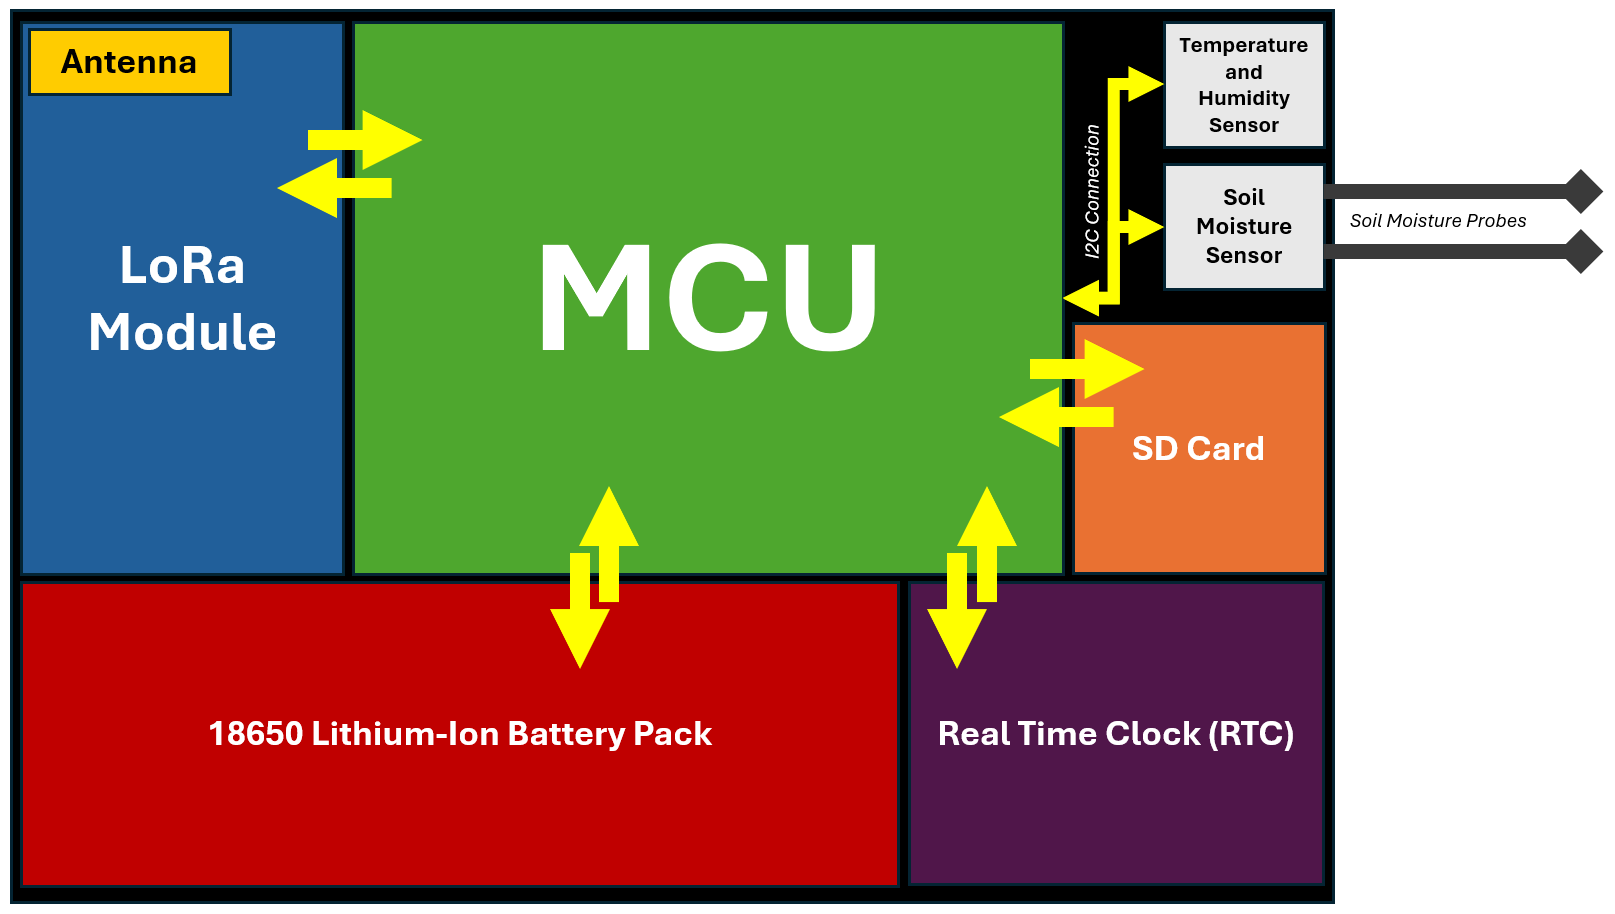
\includegraphics[width=5.48053in,height=3.10153in]{figs/method-image2.png}
\end{figure}

\subsubsection{Device Components}

\subsubsection{LoRa Module (Ra-02 SX1278
433Mhz)}

The Ra-02 LoRa module, based on the SX1278 transceiver,
operates at 433 MHz, which is within the legal ISM band in Iceland. The
module offers long-range communication capabilities of up to several
kilometers, which is more than sufficient for the expected distances
between turf houses. Additionally, the module has low power consumption
and a small physical footprint, making it suitable for a compact and
energy-efficient sensor node
design.


\subsubsection{Microcontroller (Arduino Pro
Mini)}

The choice of microcontroller was a critical design decision.
The microcontroller needed to be compact, energy efficient, and capable
of handling sensor data acquisition, storage, and wireless
communication. Several alternatives were considered, including the
ESP32; however, it was deemed unsuitable due to higher power
consumption, higher cost, and excess computational capability for the
requirements of this
project.


The Arduino Pro Mini, based on the ATmega328P
microcontroller, was selected as it operates at 3.3 V with an 8 MHz
clock frequency and provides 32 kB of flash memory. It supports both I2C
and serial communication, which are required for interfacing with the
sensors and peripheral modules. The available memory and processing
capability were found to be sufficient for the application. Power
consumption is approximately 4.5 mA during active operation and can be
reduced to approximately 3 µA in deep sleep mode after removing onboard
indicator LEDs, which was implemented in this
project.


\subsubsection{Air Temperature and Humidity Sensor
(AHT10)}

The AHT10 sensor was selected for measuring air temperature
and humidity due to its availability, low cost, and adequate accuracy
for the application. The sensor communicates via the I2C interface and
is capable of measuring temperatures from −40 °C to 85 °C with an
accuracy of ±0.3 °C. Relative humidity measurements range from 0\% to
100\% with an accuracy of ±2\%, which is sufficient for monitoring
environmental conditions beneath turf
roofs.


\subsubsection{Soil Temperature Sensor
(DS18B20)}

The DS18B20 digital temperature sensor was selected for soil
temperature measurements due to its simplicity, accuracy, and
robustness. The sensor operates over a temperature range of −55 °C to
125 °C with an accuracy of ±0.5 °C. It communicates using a one-wire
interface, requiring only three connections, which simplifies wiring and
reduces complexity. Waterproof probe-style versions of the DS18B20 are
widely available, making the sensor well suited for buried soil
applications.


\subsubsection{Soil Moisture Sensor (Capacitive Soil Moisture
Sensor
v1.2)}

A generic off-the-shelf capacitive soil moisture sensor (v1.2) was used
in this study. The sensor design is open source and widely available,
resulting in many similar commercial versions. This sensor outputs an
analog voltage that varies with the soil moisture content, which is read
by the Arduino as an analog value within the range defined by the 3.3 V
supply voltage. Despite being low cost, previous studies have shown that
capacitive soil moisture sensors can provide consistent and reliable
measurements when properly selected and calibrated, as discussed in
Chapter 2.

Capacitive sensors were chosen over resistance-based alternatives due to
their improved reliability and reduced susceptibility to corrosion in
moist soil environments. While professional-grade soil moisture
measurement methods such as TDR and FDR offer higher accuracy, they are
significantly more expensive and less suitable for large-scale
deployment. In contrast, low-cost capacitive sensors offer a practical
solution for distributed monitoring applications, such as turf roof
installations.

In this study, the selected sensor was used with the understanding that
calibration is required to improve measurement accuracy. By calibrating
the sensor against professional-grade reference instruments, the system
aims to achieve accurate soil moisture measurements while maintaining
low cost and scalability.

\subsubsection{SD Card Module (SparkFun OpenLog Serial
Logger)}

Local data storage was implemented using the SparkFun OpenLog
serial logger module. Several SD card modules were initially evaluated;
however, many were found to be too large, power intensive, or required
software libraries that exceeded the available flash memory of the main
microcontroller.


The OpenLog module records data received over a serial
interface directly to a microSD card and is based on its own ATmega328
microcontroller, allowing it to operate independently of the main MCU.
This approach significantly reduces memory usage on the sensor node. The
module supports microSD cards up to 32 GB and consumes approximately
2--6 mA during operation, making it suitable for low-power data
logging.


\subsubsection{Power Source (18650 Samsung 35E 3500mAh Li-Ion
Battery)}

The system is powered using three 18650 lithium-ion
batteries, each with a nominal capacity of 3500 mAh, providing a total
capacity of 10,500 mAh. These batteries operate over a voltage range of
approximately 2.65 V to 4.2 V, which is suitable for a 3.3 V
system.


To ensure safe operation within voltage limits, a Zener diode
is used to reduce the maximum input voltage by approximately 0.5 V. This
configuration ensures compatibility with the 3.3 V power requirements
while providing sufficient capacity for long-term
operation.


Size was an important consideration in the design of the sensor modules.
However, sourcing batteries with a small form factor and high capacity
was severely limited by import fees, availability, and cost. As a
result, a conventional and widely available 18650 lithium-ion battery
was selected.

\subsubsection{Real Time Clock
(DS3231)}

The DS3231 real-time clock was selected due to its high accuracy, low
power consumption, and integrated temperature-compensated crystal
oscillator. The module includes a battery backup and consumes
approximately 100 µA in standby mode. It supports up to two programmable
alarms capable of generating an interrupt signal, which is used to wake
the microcontroller from deep sleep mode.

This functionality is critical for synchronizing sensor nodes and
ensuring consistent data collection and transmission intervals across
the mesh network.

\subsubsection{Antenna (433Mhz
3dbi)}

The selected antenna operates at 433 MHz, which matches the
configuration of the system. The antenna has a minimal design and is
commonly used for radio communication applications, making it suitable
for LoRa operation. Although the antenna has a gain of only 3 dBi, it
provides significantly better performance than operating without an
external antenna.

Additionally, the antenna's compact and discreet design allows it to
blend well with the surrounding environment. Its small size and vertical
form factor make it visually unobtrusive, resembling tall grass, which
is important for maintaining the stealth and aesthetic requirements of
the turf roof installation.

\subsubsection{Schematic Design}

This section describes the schematic design of the main
printed circuit board (PCB) used for the sensor node. To compactly
integrate all components into the smallest possible form factor and to
simplify assembly and wiring, a custom PCB was designed and
manufactured. The PCB houses all system components described in the
previous section, with the exception of the batteries, along with
additional circuitry required for system
functionality.


\subsubsection{\begin{figure}[htbp]
\centering
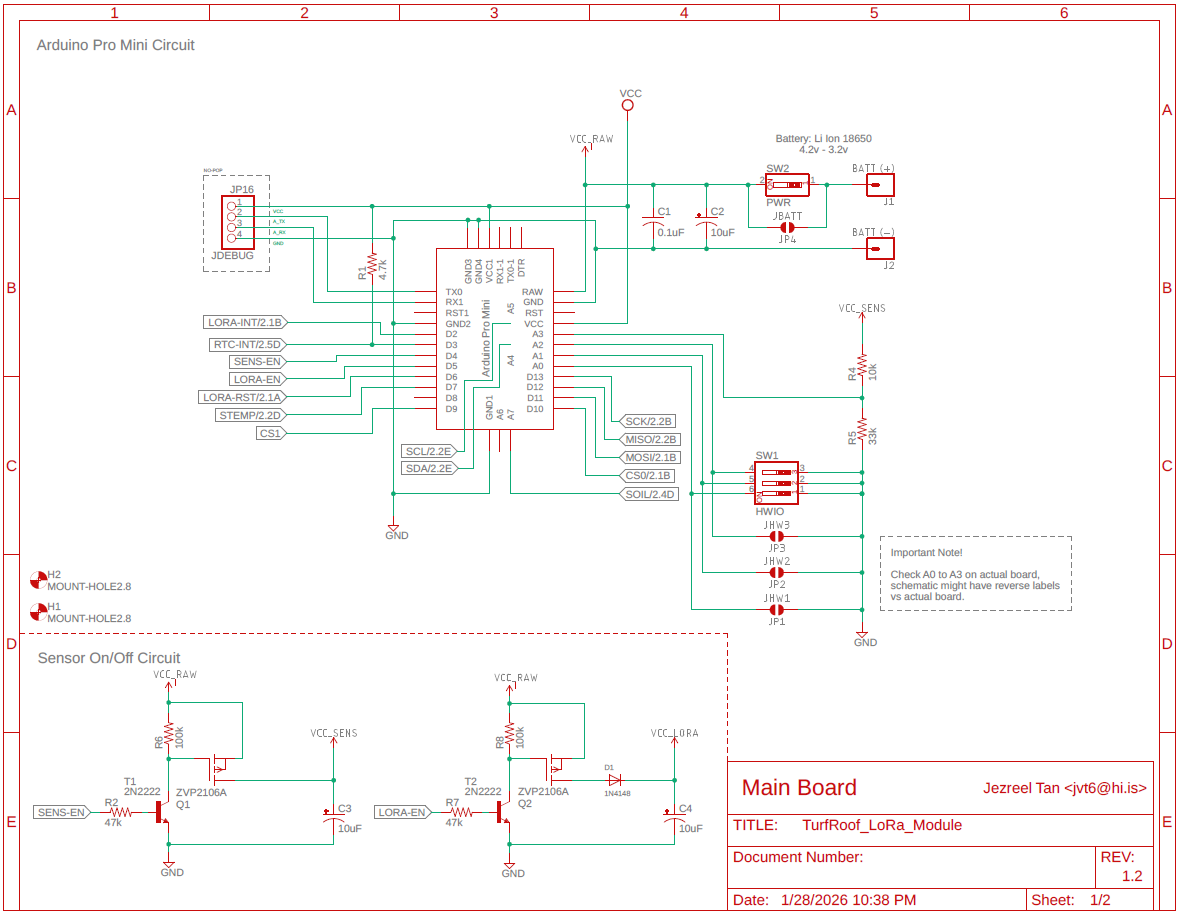
\includegraphics[width=5.43347in,height=4.22139in]{figs/method-image3.png}
\end{figure}}

Battery voltage monitoring is implemented using a simple voltage divider
connected to analog pin A3 of the microcontroller. The microcontroller
reads the divided voltage as an analog value, which is then converted
back to the corresponding battery voltage in software. This allows the
system to monitor battery health during operation.

To minimize power consumption during sleep periods, the design includes
MOSFET-based power control for two sensor groups, labeled SENS-EN and
LORA-EN. When the system enters deep sleep mode between data collection
intervals, the microcontroller disables both MOSFETs, effectively
cutting power to the sensors and the LoRa module. Each group is only
powered when required and is turned off immediately afterward, ensuring
minimal power consumption during inactive periods.

\subsubsection{Hardware ID}

As shown in the schematic, the core of the board is the Arduino Pro Mini
microcontroller. A component labeled SW1 is used as a three-bit hardware
identifier, allowing each sensor node to be assigned a unique ID. Upon
boot, the microcontroller reads the state of these bits and assigns the
corresponding hardware ID to the node, preventing data collisions during
transmission. With this configuration, up to seven unique devices can be
supported within a single system. The design can be further scaled by
adding additional identifier bits using available microcontroller pins.
For deployments involving multiple systems, software-based hardware
prefixes can be implemented to distinguish between different system
groups.

\begin{figure}[htbp]
\centering
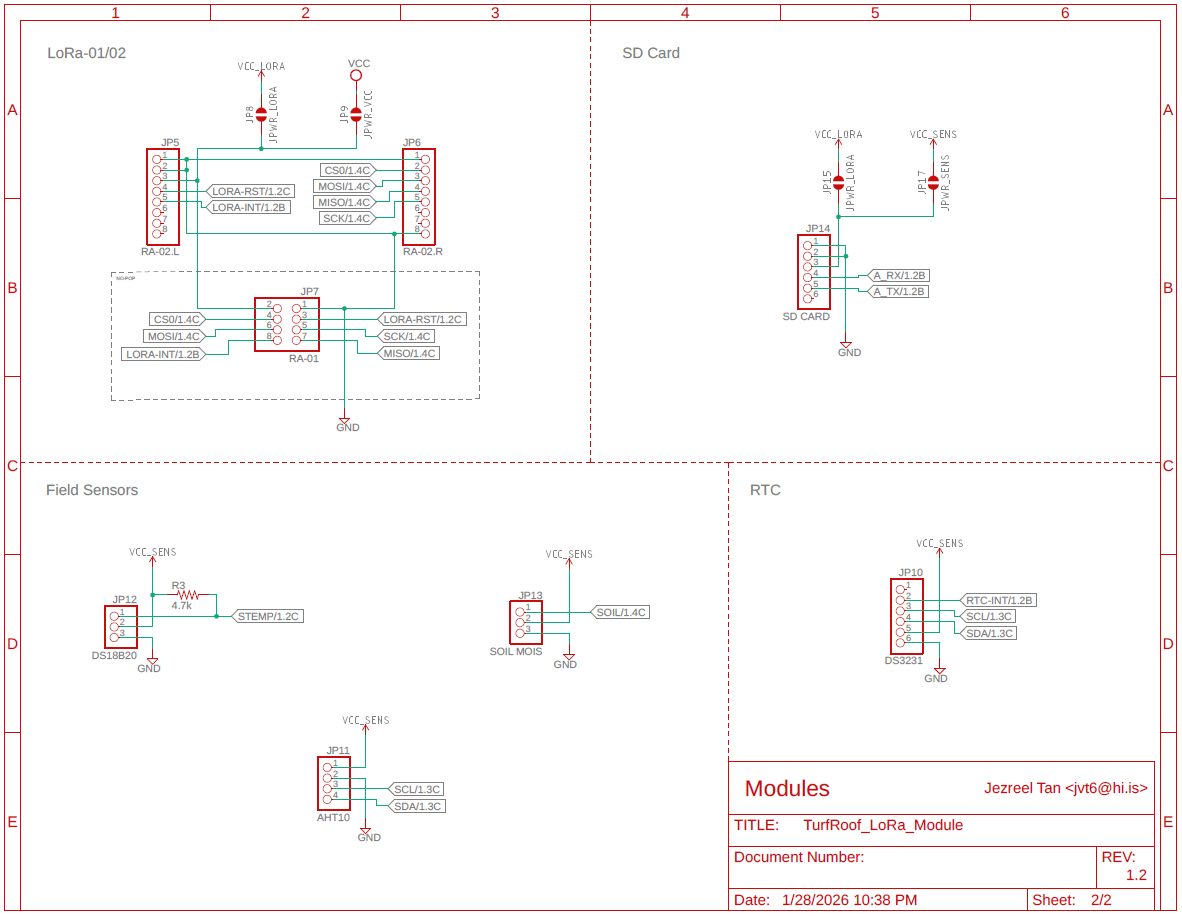
\includegraphics[width=5.59929in,height=4.33885in]{figs/method-image4.png}
\end{figure}

The PCB layout was primarily designed to accommodate the Ra-02 LoRa
module. However, based on feedback from users with experience in LoRa
systems, an alternative module package (Ra-01), which offers similar
specifications but a different form factor, was also considered. To
support this flexibility, a no-populate drop-in footprint was included
on the PCB, allowing either module to be used depending on availability
or user preference.

For the sensor interfaces, pin headers were used to simplify the design,
testing, and development process. This approach allows sensors to be
easily connected and disconnected, improving ease of assembly and
enabling quicker replacement or modification during testing and
deployment.

\subsubsection{PCB Design and
Manufacturing}

During the PCB design process, cost and compactness were carefully
considered. The main PCB for a single sensor module was designed to fit
within a 50.5 mm × 50.5 mm footprint using a two-layer, 1.6 mm thick
FR-4 substrate. A two-layer design was sufficient due to the relatively
low routing complexity, helping to reduce manufacturing costs.

The PCB was manufactured by JLCPCB. Ground planes were incorporated
where possible to improve signal integrity and reduce noise,
particularly around the LoRa transceiver. Component placement was
optimized to allow ease of manual assembly and debugging during
development.

The use of pin headers for the sensors simplified the assembly process,
allowing sensors to be rearranged easily and packed neatly within the
enclosure.

\begin{figure}[htbp]
\centering
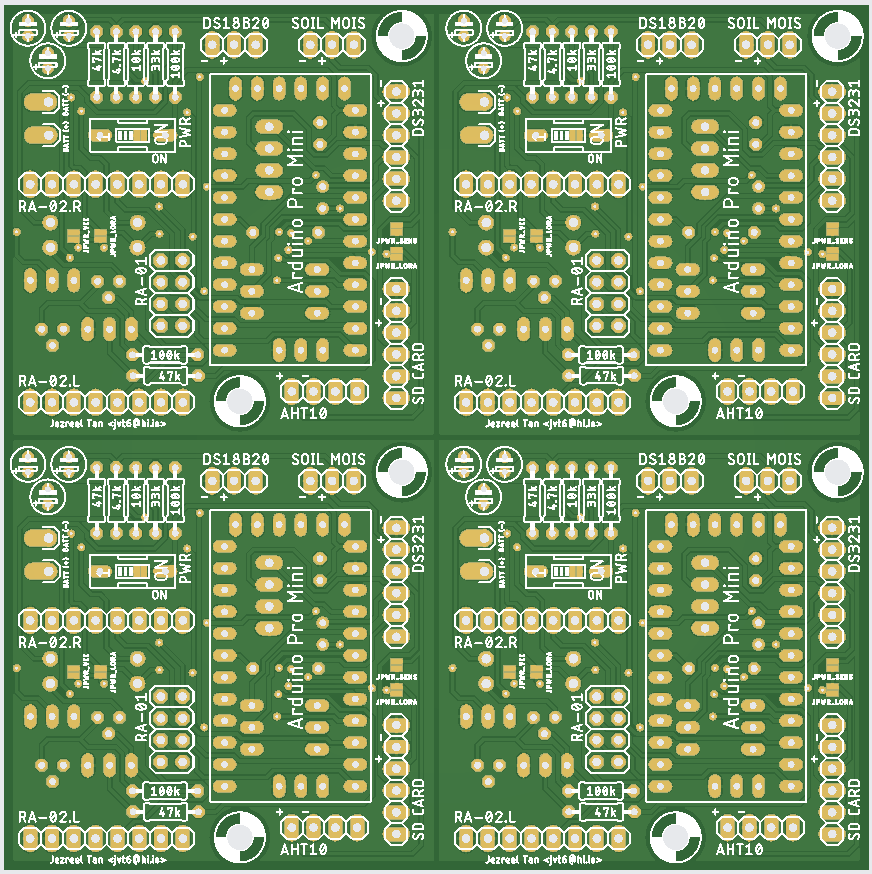
\includegraphics[width=3.84123in,height=3.84985in]{figs/method-image5.png}
\end{figure}

\subsubsection{System Assembly}

To ensure reliable operation under the harsh environmental conditions in
Iceland, all sensor components were enclosed in a weatherproof and
waterproof housing. The components were assembled neatly inside the
enclosure to protect them from moisture, rain, snow, and temperature
variations. Although the initial goal was to minimize the size of the
sensor module---ideally approaching the size of the main PCB---the
batteries were the primary limiting factor in reducing the overall form
factor. Nevertheless, the final design remained compact, easy to handle,
and capable of housing sufficient battery capacity for long-term
operation.

Two enclosure designs were developed and evaluated to determine which
configuration provided better performance and practicality. The first
design integrated the LoRa antenna directly into the main sensor
enclosure. This resulted in a more compact and mechanically robust
module with fewer loose components. However, this configuration limited
flexibility during installation, particularly in confined or uneven
mounting locations.

The second design utilized an external waterproof enclosure connected
via a cable, housing both the LoRa antenna and the AHT10 air temperature
and humidity sensor. This configuration allowed the air sensor to be
positioned above ground, resulting in more representative air
temperature and humidity measurements. However, this design increased
exposure of the sensor and cabling to environmental elements, requiring
additional protection to prevent potential damage.

After assembly, all seams, cable entry points, and enclosure openings
were sealed using silicone sealant to ensure watertightness. This final
sealing step was critical in protecting the electronics from water
ingress caused by rain, snow, and meltwater, thereby improving the
overall durability and reliability of the system.

\begin{figure}[htbp]
\centering
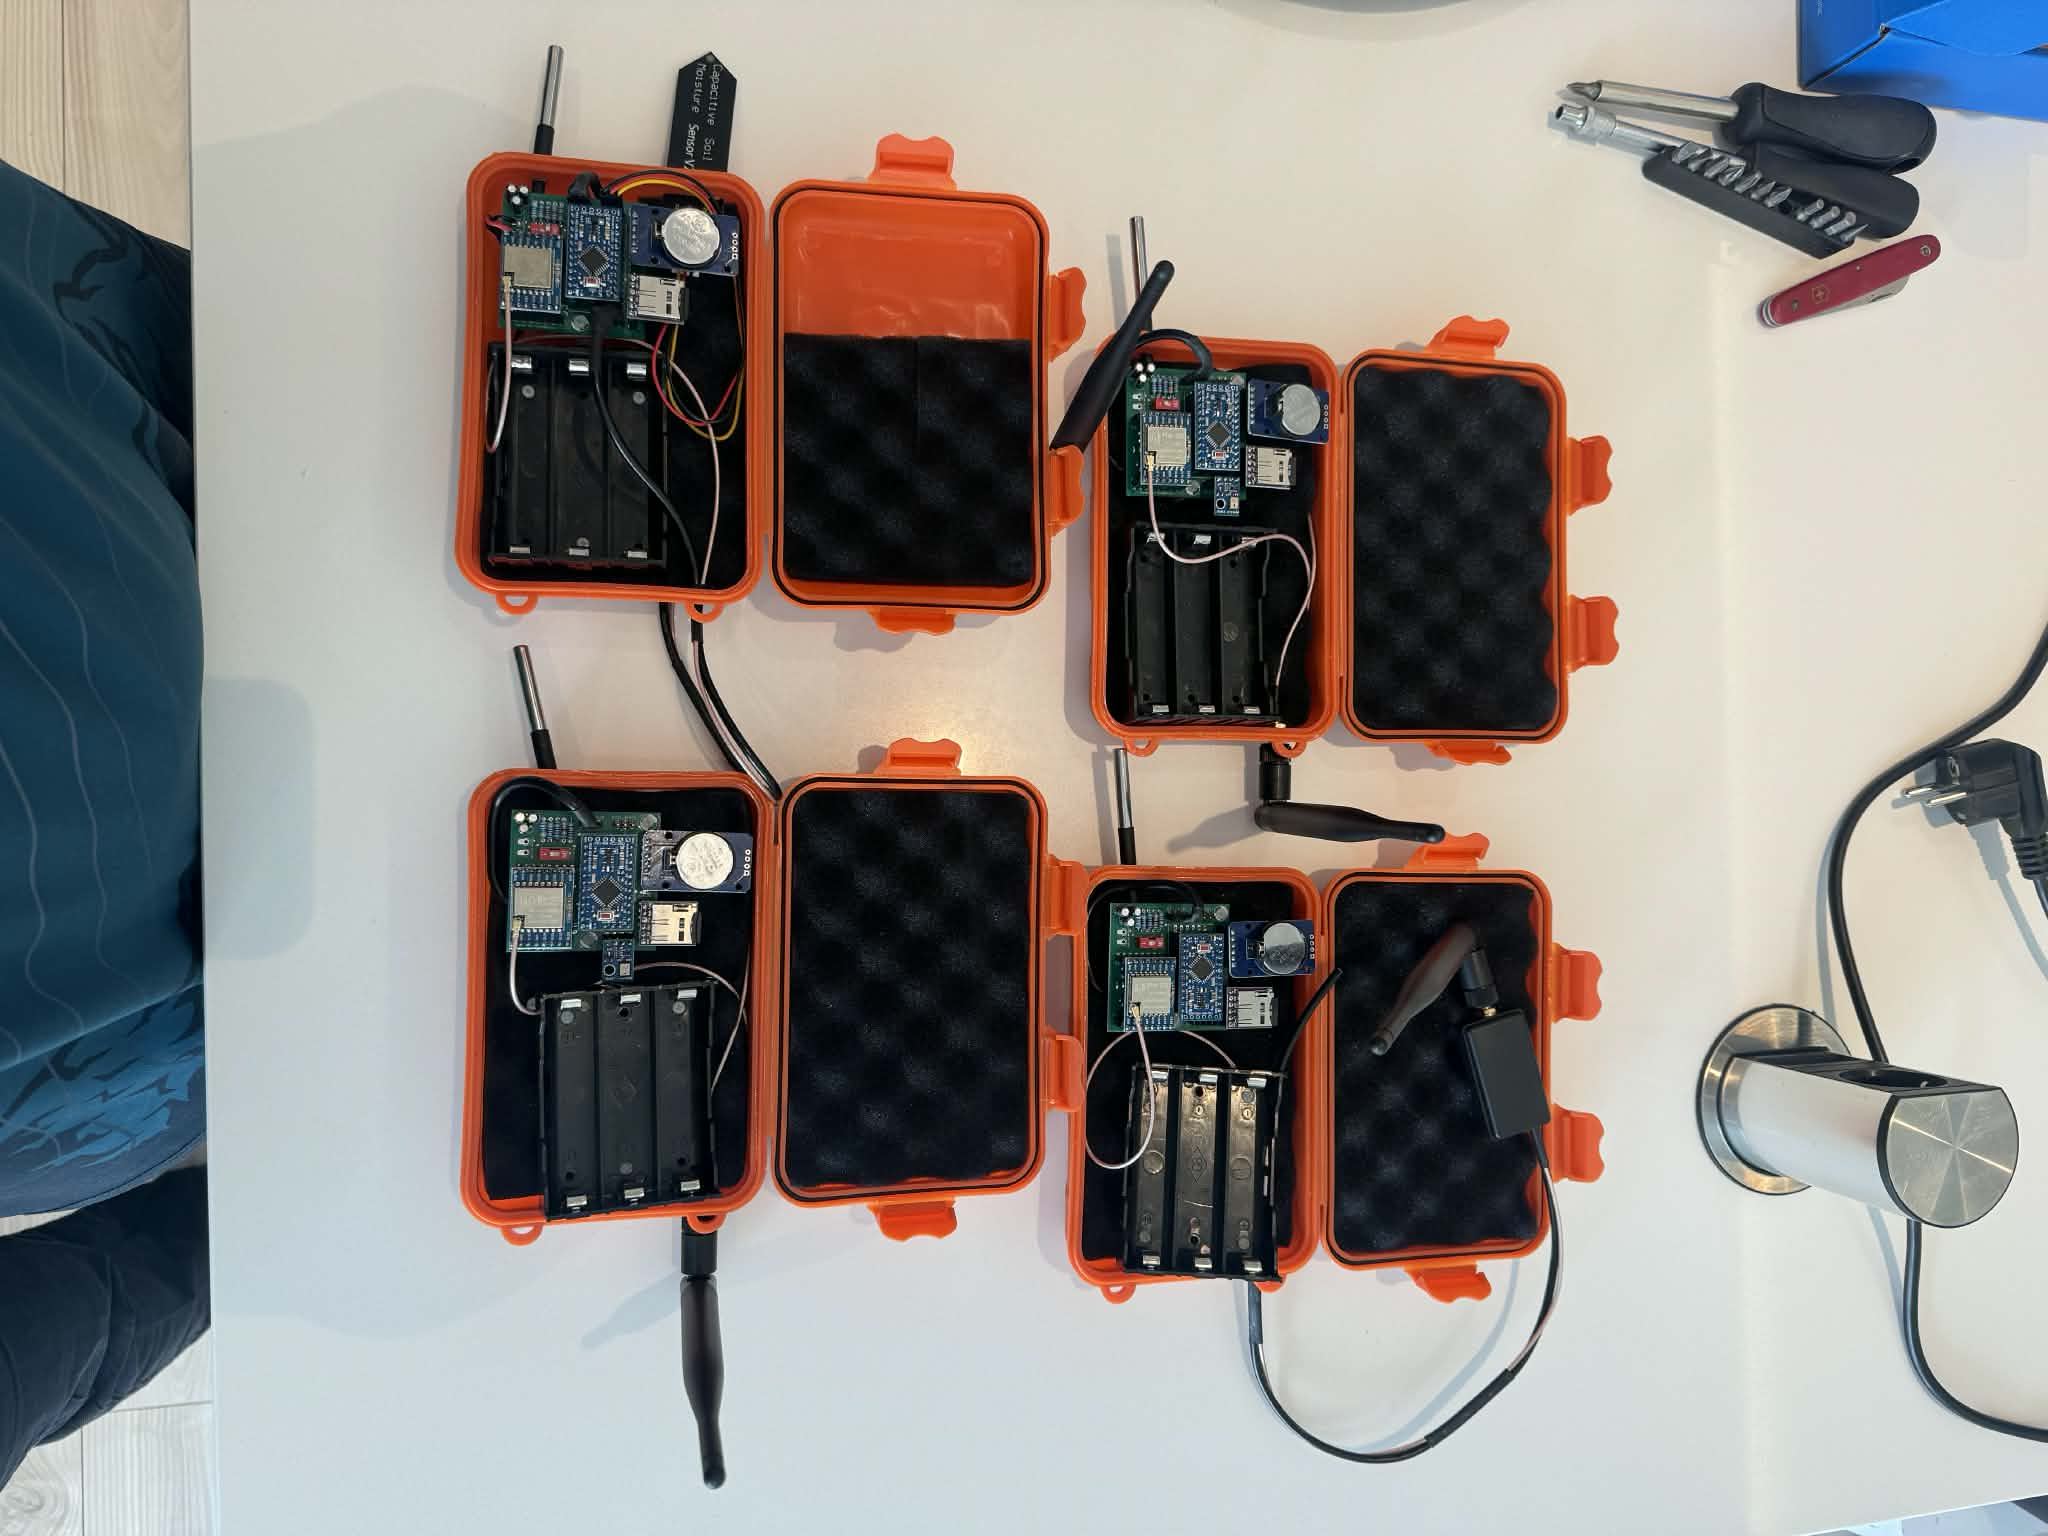
\includegraphics[width=4.33694in,height=3.25921in]{figs/method-image6.jpeg}
\end{figure}

\subsection{Base Station Module}

The base station module consists of a low-power microcontroller unit
(MCU) and a LoRa module. The MCU connects directly to the internet via
Wi-Fi to synchronize time and is powered through a mains outlet to
ensure a stable and continuous power supply. Using its internal clock,
the MCU enters sleep mode between intervals and periodically checks the
time through the internet to ensure accurate wake-up timing.

At scheduled intervals, the base station MCU sends a signal to all
sensor nodes to initiate data collection. At this time, all sensor nodes
are expected to be awake and ready to transmit data. Once the base
station receives all required data, it broadcasts the current date and
time to ensure that all sensor nodes remain time-synchronized. This
process allows the sensor nodes to be synchronized on an hourly basis.

After synchronization, the base station uploads the collected data to
the cloud, where it is stored and made available for viewing and further
data analysis by researchers.

\begin{figure}[htbp]
\centering
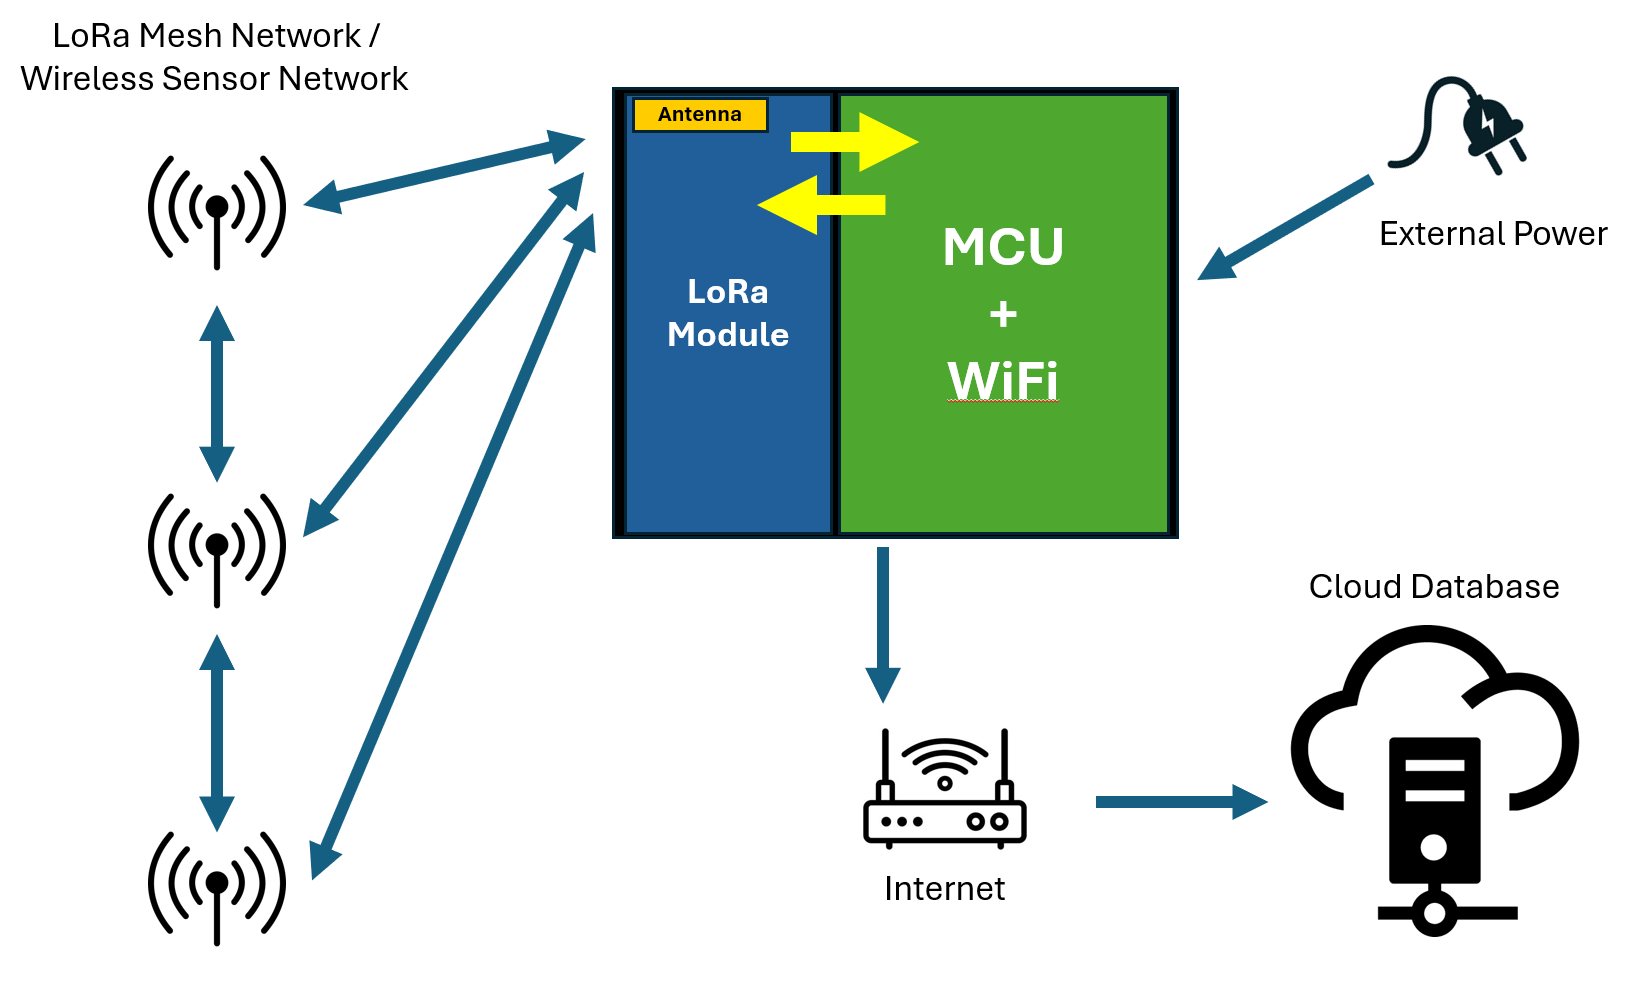
\includegraphics[width=\textwidth]{figs/method-image7.png}
\end{figure}

\subsubsection{Device Components}

\subsubsection{LoRa Module (Ra-02 SX1278
433Mhz)}

The base station uses the same Ra-02 LoRa module as the
in-situ sensor nodes to maintain consistency across the system. Using
the same LoRa module simplifies system design, firmware development, and
communication compatibility between the base station and sensor nodes.
Additionally, this approach reduces component variation and ensures
reliable and uniform communication performance throughout the
network.

\subsubsection{Microcontroller (LOLIN D1
mini)}


Initially, during the concept design and planning stage, a Raspberry Pi
was considered as the primary choice for the base station. Based on a
review of similar theses and related projects, many researchers used a
Raspberry Pi for comparable applications. However, after further
development and evaluation, it was concluded that a Raspberry Pi would
be excessive for the requirements of this system. In addition, it is
relatively costly, and several lower-power microcontroller-based
alternatives were found to be more suitable for the application.

Eventually, the LOLIN D1 mini was selected as the base station
controller. The board is based on the ESP8266EX chip, which provides
built-in Wi-Fi connectivity. It supports SPI communication, which is
required for interfacing with the LoRa module, and operates at 3.3 V
with an 80 MHz clock frequency and 4 MB of flash memory. These
specifications were sufficient for the data handling, communication, and
synchronization tasks of the base station. The board can be programmed
using C/C++, allowing efficient use of its limited flash memory and
providing flexibility for firmware customization. Additionally, the
module can be easily powered through a USB Type-C connection, enabling
the use of common power adapters for continuous operation.


\subsubsection{System Assembly}

The base station module has a relatively simple hardware configuration,
which made assembly and integration straightforward. Since both the
microcontroller and the LoRa module operate at 3.3 V, they can be
directly interconnected without the need for additional level-shifting
circuitry. The SPI communication lines were connected between the MCU
and the LoRa module, and the antenna was securely attached to the LoRa
module to ensure proper radio performance.

Power was supplied to the base station through a mains-powered adapter,
allowing continuous operation without power constraints. After assembly,
the microcontroller was programmed with the base station firmware, and
basic functionality was verified. Proper antenna installation was
ensured to avoid signal degradation during operation.

\section{Firmware}

The firmware for the proposed LoRa mesh wireless sensor network was
developed in C/C++ using an object-oriented programming (OOP) approach.
The system is based on the ATmega328P microcontroller, which is
well-supported within the Arduino development ecosystem and allows
efficient low-level hardware control. An object-oriented structure was
selected to improve modularity, scalability, and maintainability of the
system. By encapsulating functionality into separate classes (e.g.,
sensor handling, LoRa communication, data management, and power
control), the firmware becomes easier to debug, extend, and adapt for
future deployments or additional sensing requirements.

\begin{quote}
Firmware development and flashing were performed using the Arduino IDE.
Arduino was selected because of its open-source architecture,
comprehensive library support, and strong developer community, which
streamline firmware development, enable efficient debugging, and provide
flexibility for future system expansion. Standard Arduino libraries were
utilized where appropriate, including libraries for SPI communication
(LoRa module), I2C communication (environmental sensors), SD card
interfacing, and low-power sleep control. Custom logic was implemented
to manage mesh routing, data formatting, packet handling, and power
optimization.

Two primary firmware implementations were developed:
\end{quote}

\begin{enumerate}
\def\labelenumi{\arabic{enumi}.}
\item
  \textbf{In Situ Sensor Node Firmware} -- responsible for sensor data
  acquisition, packet formatting, mesh communication, local data backup,
  and low-power operation.
\item
  \textbf{Base Station Firmware} -- responsible for receiving and
  decoding mesh packets, managing acknowledgments, and uploading
  validated data to the cloud platform.
\end{enumerate}

\begin{quote}
The full source code repository is publicly available at:\\
\url{https://github.com/JezT25/turfroof_lora}
\end{quote}

\subsection{The LoRa Mesh System}

During the early stages of algorithm development, particular attention
was given to how sensor data could be distributed evenly, reliably, and
robustly across the mesh network. The primary objective was not only to
ensure that the base station received all measurements, but also to
enhance network resilience by reducing dependence on a single
communication path.

An architectural concept inspired by distributed ledger systems, such as
blockchain, influenced the final design. In blockchain systems, a shared
ledger acts as a synchronized and verifiable record of transactions
across multiple participants, ensuring consistency and integrity of
data. While the proposed system does not implement blockchain or
cryptographic consensus mechanisms, it adopts a simplified
distributed-ledger-inspired approach to improve robustness within the
LoRa mesh network.

In this implementation, the base station initializes a structured data
ledger template, which is propagated throughout the network. Each sensor
node appends its most recent measurement to the ledger before forwarding
it to neighboring nodes. Through multi-hop transmission, the ledger
circulates across the mesh until all participating nodes have
contributed their respective data entries.

This approach ensures that:

\begin{itemize}
\item
  Data redundancy is introduced at the network level.
\item
  Nodes can verify whether their measurements have been successfully
  incorporated.
\item
  The system reduces single points of failure.
\item
  Network robustness is improved in the event of intermittent
  connectivity.
\end{itemize}

By allowing all nodes to maintain awareness of the aggregated dataset
before final transmission to the base station, the system achieves
greater reliability compared to a traditional star topology where only
the base station holds the complete dataset. The final validated ledger
is then transmitted to the base station for cloud upload and long-term
storage.

\subsubsection{Architecture}

To simplify debugging and system validation during development, all LoRa
data packets were transmitted as human-readable plaintext strings.
Although this approach is less efficient than using compact binary
packet structures, it significantly improved transparency during early
testing and troubleshooting. Being able to directly inspect transmitted
data without additional decoding tools allowed for faster identification
of routing, formatting, and communication errors within the mesh
network.

It should be noted that, for a production-level implementation, a packed
data structure (e.g., a structured binary payload containing predefined
variables) would be preferable. Such an approach would reduce payload
size, improve transmission efficiency, and optimize airtime usage ---
particularly important in low-bandwidth LoRa systems.

The decision to retain plaintext transmission in the final prototype was
primarily influenced by the system's early testing phase, where
plaintext communication was initially implemented and validated.
Maintaining this format ensured consistency and stability throughout
development. Nevertheless, future iterations of the system would benefit
from migrating to a structured binary packet format for improved
scalability and performance.

3.4.1.1.1 The Packets

To initiate communication within the mesh network, one node ---
typically the base station --- broadcasts a structured ledger packet.
This ledger acts as a container for aggregated data and is circulated
among all participating nodes. The packet consists of three main
components: a header, reserved data fields for each node, and a checksum
value used for basic integrity verification.

Each node in the network is assigned a unique hardware ID. This ID
determines the fixed position within the packet where the node inserts
its data. For example, if a node has a hardware ID of 3, it writes its
measurement into the fourth allocated data field within the ledger. This
positional mapping prevents data overwriting and ensures deterministic
placement of measurements, allowing every node to know exactly where its
contribution belongs within the packet.

Because all data is transmitted in plaintext format, each node is
allocated a fixed number of characters. While a packed binary structure
with defined variable types would have been more memory-efficient and
flexible, fixed-width plaintext fields were chosen to simplify
debugging, inspection, and demonstration of the system. Each numerical
value is formatted to support a range from --99.9999 to 999.9999. This
range comfortably accommodates all measured parameters (e.g.,
temperature, humidity, soil moisture, battery voltage), ensuring no
overflow occurs within the defined field size.

To maintain low computational overhead on the ATmega328P
microcontroller, the checksum mechanism was intentionally simplified.
Instead of implementing a standard CRC16 or similar algorithm, the
checksum is computed as the arithmetic sum of numerical values from node
0 through node 7. While this does not provide the robustness of
industry-standard CRC implementations, it offers a lightweight integrity
check suitable for the processing and memory constraints of the
hardware.

All data entries are comma-separated and enclosed within brackets
({[}{]}), forming a predictable and easily parseable structure. The
packet header defines the type of data being transmitted, such as air
temperature, relative humidity, soil temperature, soil moisture, battery
voltage, or time/date synchronization.

\begin{figure}[htbp]
\centering

\includegraphics[width=\textwidth]{figs/method-image8.png}
\end{figure}

Time/date packets follow a slightly modified format. Instead of
allocating separate fields per node, the packet's data fields are used
collectively to distribute synchronized timestamp information across the
network. This mechanism ensures that all nodes maintain consistent
system time for logging and coordination purposes.

\begin{figure}[htbp]
\centering

\includegraphics[width=\textwidth,height=0.41875in,keepaspectratio]{figs/method-image9.png}
\end{figure}

In total, each packet occupies 97 characters (97 bytes). Although
plaintext transmission simplifies inspection, it inherently lacks
confidentiality. To provide a basic level of security, packets are
encrypted prior to transmission using the RC4 stream cipher. RC4 was
selected due to its lightweight computational requirements and minimal
memory footprint, making it suitable for the ATmega328P's limited RAM
and processing capability.

An initial implementation using AES encryption was considered; however,
it proved too computationally intensive for the microcontroller. AES
encryption introduced noticeable delays in packet preparation, which
negatively impacted mesh responsiveness and routing performance. Given
the constrained resources of the ATmega328P, RC4 provided a practical
compromise between security and system efficiency.

3.4.1.1.2 RC4

The implemented function follows the standard RC4 structure, consisting
of a key scheduling phase and a pseudo-random generation phase. A state
array is initialized and permuted using the predefined ENCRYPTION\_KEY.
During encryption, a pseudorandom byte (rnd) is generated and XORed
directly with each byte of the data buffer. Because RC4 is symmetric,
the same function is used for both encryption and decryption. To
conserve RAM, the implementation limits the state array to 255 bytes
instead of the conventional 256, reducing memory consumption while
maintaining functional encryption for this prototype. Although RC4 is
not considered secure for high-security applications due to known
vulnerabilities, it provides sufficient packet obfuscation for this
research deployment where low power consumption and computational
efficiency are prioritized.

The implemented function is shown below:

\begin{figure}[htbp]
\centering
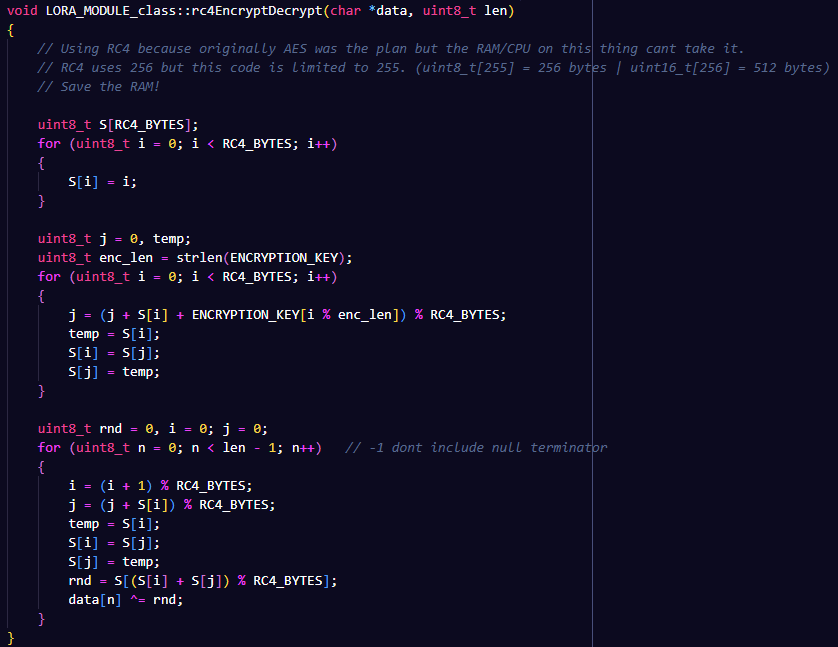
\includegraphics[width=\textwidth,height=5.01875in,keepaspectratio]{figs/method-image10.png}
\end{figure}

\textless talk about the picture here more\textgreater{}

\subsubsection{Mesh Network}

Once a ledger is transmitted, any node within range can receive it,
provided that it is properly formatted. Upon reception, the node
decrypts the packet, extracts the data, and compares it with its local
database. The node then updates its local database using the data from
the received ledger and updates the ledger using its own stored data.
After updating, the ledger may be relayed to other nodes to allow them
to update their respective databases. This process continues until all
nodes possess a fully updated ledger.

Relaying is not automatically performed for every received packet. If
unconditional relaying were implemented, the mesh network would fall
into an infinite rebroadcast loop. Before relaying a ledger, the node
must determine whether retransmission is necessary. If a node receives a
ledger that differs from its local database, it indicates that at least
one node in the network is missing data. In this case, the receiving
node updates the ledger using its local database and relays it, ensuring
that the node which originally transmitted the incomplete ledger
eventually receives the updated information.

For example, if Node 3 receives a ledger that does not contain data from
Node 3, it can infer that somewhere in the network there exists a node
that does not have Node 3's data. Node 3 then updates the ledger and
relays it. This mechanism is not limited to the node's own data. If Node
3 receives a ledger missing Node 5's data, but Node 3 already has Node
5's data stored locally from a previous transmission, Node 3 can update
the ledger and retransmit it. This eliminates the need for the data to
travel multiple hops back to Node 5 before being redistributed,
improving overall efficiency.

The only situation in which a node does not relay a ledger is when the
received ledger is identical to its local database. In this case, all
participating nodes already possess the same data, and retransmission
would only create unnecessary traffic and potential infinite looping.
Therefore, the packet is ignored.

\begin{figure}[htbp]
\centering
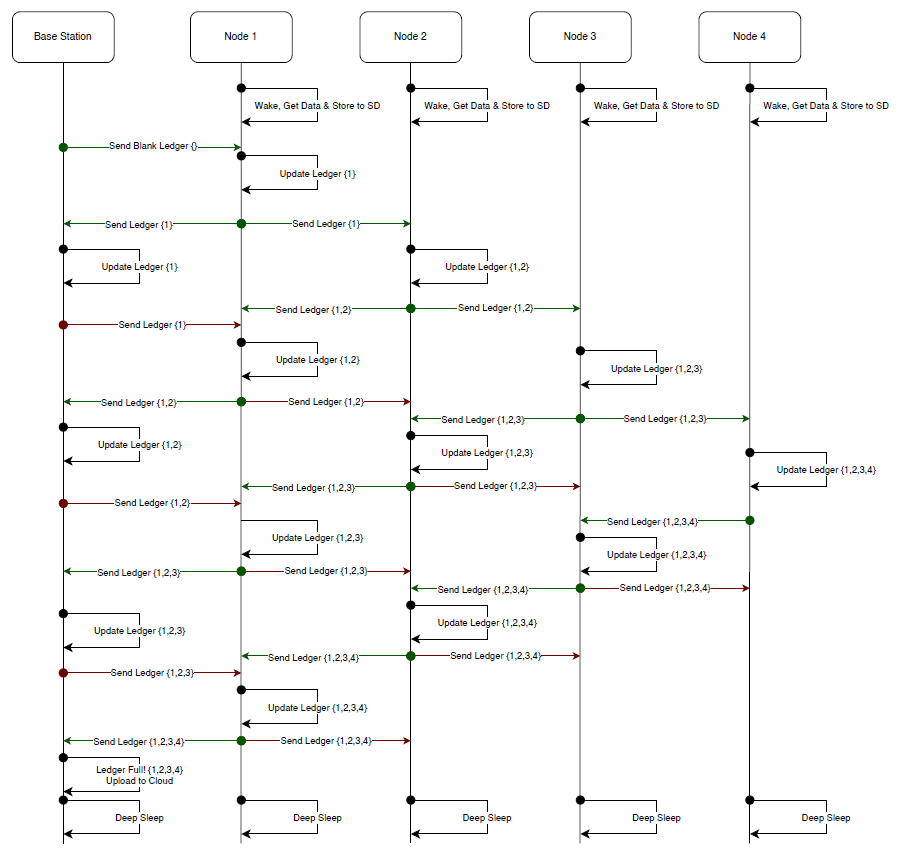
\includegraphics[width=4.43591in,height=4.23923in]{figs/method-image11.png}
\end{figure}

In a linear topology scenario, the base station may only be within range
of Node 1; Node 1 within range of the base station and Node 2; Node 2
within range of Node 1 and Node 3; and so forth. When the base station
sends a packet, Node 1 receives it, updates the ledger, and retransmits
it to nodes within range. This creates a chain reaction until the last
node updates the ledger. The fully updated ledger then propagates back
toward the base station through another chain reaction. Once the base
station receives the complete ledger, the data is saved and uploaded to
the cloud.

\subsubsection{Dealing with Collisions (CSMA/CA (Carrier Sense Multiple Access with Collision Avoidance))}


To prevent simultaneous transmissions that may cause packet collisions,
Carrier Sense Multiple Access with Collision Avoidance (CSMA/CA) is
implemented. Since the LoRa module cannot transmit and receive at the
same time, collision avoidance is necessary to ensure reliable
communication.

Before transmitting, a node first checks the LoRa channel noise level.
If the channel is busy, indicating that packets are currently being
transmitted, the node waits until the channel becomes idle before
attempting to send. This reduces the probability of collision.

However, a node cannot wait indefinitely. Therefore, a timeout mechanism
is implemented. If all nodes were assigned identical timeout values,
collisions could still occur when timeouts expire simultaneously. To
avoid this, each node multiplies the base timeout value by its hardware
ID. This ensures that each node has a different timeout duration. In the
worst-case scenario where all nodes intend to transmit and reach their
timeout, transmissions will occur at different times due to the hardware
ID multiplier.

Additionally, if a node receives a valid packet while waiting to
transmit, it reevaluates the received packet, updates or discards it
accordingly, and restarts its timeout counter. This effectively delays
its transmission and reduces the likelihood of congestion. This
mechanism ensures that channel noise decreases before additional packets
are introduced.

\begin{figure}[htbp]
\centering
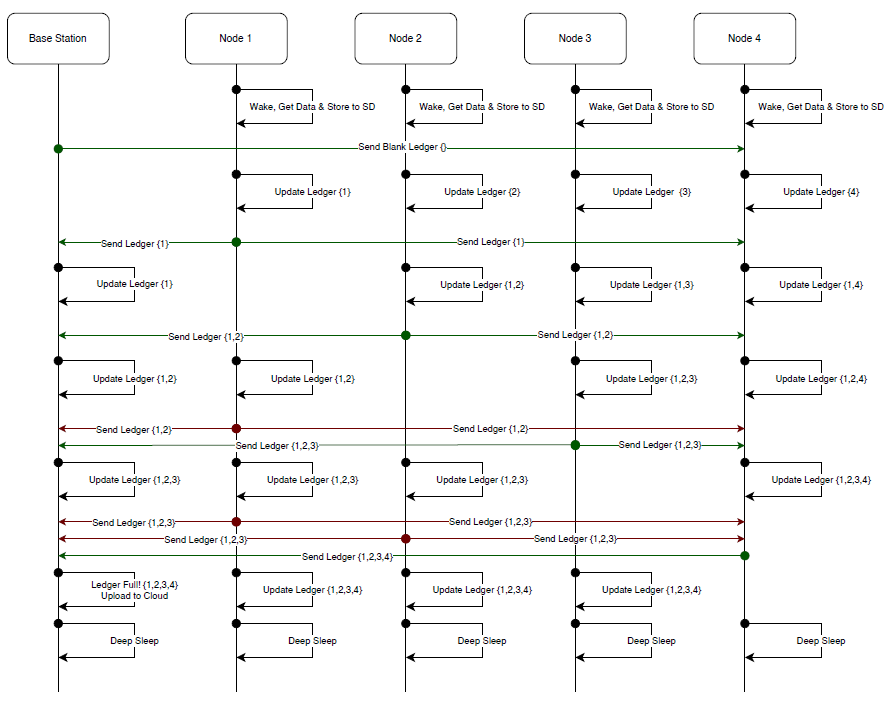
\includegraphics[width=\textwidth,height=5.16528in,keepaspectratio]{figs/method-image12.png}
\end{figure}

In a scenario where all nodes are within range of each other, meaning a
single transmission is received by all nodes, those with lower hardware
IDs transmit first due to shorter timeouts. For example, once all nodes
update their local databases, Node 1 (with the lowest ID) transmits
first. Upon receiving Node 1's transmission, all other nodes stop their
pending transmissions, update their databases, and restart their timeout
process. This continues sequentially until all nodes have shared their
data and the base station receives the complete dataset for upload to
the cloud.

Although this collision avoidance mechanism significantly reduces packet
collisions, it is not perfect. There may be rare timing conditions where
two nodes synchronize unintentionally and transmit simultaneously.
However, due to the mesh structure of the network, the loss of a single
packet is recoverable. Since data is continuously relayed among nodes,
missed information can be recovered from neighboring nodes in subsequent
transmissions.

3.x.x.x.x Lora Firmware Settings (legal standards)

\begin{figure}[htbp]
\centering
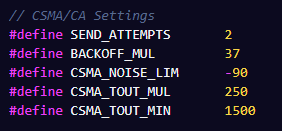
\includegraphics[width=2.93791in,height=1.36477in]{figs/method-image13.png}
\end{figure}

\textless talk about settings here and why they were chosen and legal
limits of how much sending is allowed\textgreater{}

\subsection{In Situ Sensor Behavior and
Algorithm}

The in situ node operates in a low-power duty cycle. It enters deep
sleep mode, wakes up using an RTC timer, gathers sensor data, transmits
data to the mesh network, and then returns to deep sleep. This cycle
repeats continuously throughout
deployment.\begin{figure}[htbp]
\centering
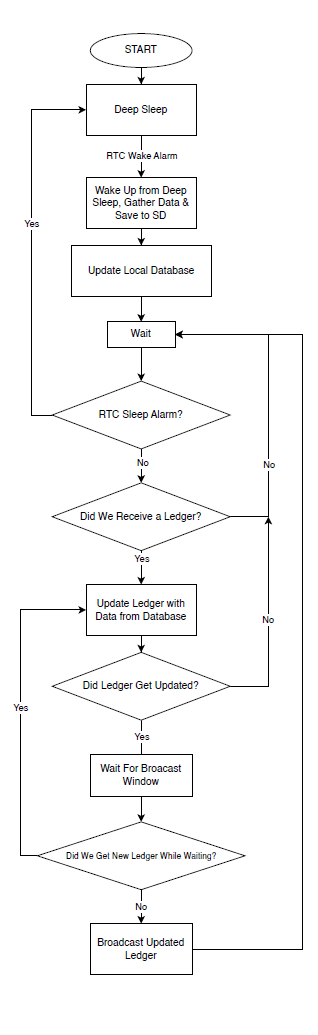
\includegraphics[width=1.36654in,height=4.44873in]{figs/method-image14.png}
\end{figure}

\subsubsection{Sensor Data Reading}

The in situ node contains multiple sensors as previously described: air
temperature and humidity, soil temperature, soil moisture, and battery
voltage. These sensors communicate using different interfaces including
I2C, 1-Wire serial, and analog-to-digital conversion (ADC).

3.4.2.1.1.Air temperature and humidity (aht10)

The AHT10 sensor communicates using the I2C protocol. The
microcontroller sends a measurement command to the sensor, after which
the sensor internally performs the necessary signal processing and
calibration. The processed temperature and humidity data are then
transmitted digitally over the I2C bus to the microcontroller. This
simplifies firmware implementation, as the sensor provides calibrated
digital output directly.

3.4.2.1.2 soil temperature

The DS18B20 soil temperature sensor communicates using the 1-Wire
protocol. Each sensor contains a unique address, allowing individual
identification if multiple sensors share the same bus. The
microcontroller initiates a temperature conversion command and reads the
digital temperature value directly from the sensor, eliminating the need
for analog calibration.

3.4.2.1.3 soil moisture

The soil moisture sensor operates on a capacitive principle. Using a
comparator-based circuit (\_\_\_ chip model), the dielectric constant of
the soil affects the sensor output voltage.

With a 3.3 V supply input, the sensor outputs an analog voltage
proportional to soil moisture. This voltage is read using the 10-bit ADC
of the ATmega328P.

ADC resolution:

\[\text{Resolution} = \frac{V_{ref}}{2^{10}} = \frac{3.3V}{1024}
\]

The raw ADC value is converted to soil moisture percentage using
calibration data obtained through the gravimetric method (see Chapter
\_\_\_).

3.4.2.1.4 battery voltage

The battery voltage is measured using a voltage divider consisting of:

\begin{itemize}
\item
  \(R_{1} = 10\text{ }k\Omega\)
\item
  \(R_{2} = 33\text{ }k\Omega\)
\end{itemize}

Voltage divider formula:

\[V_{out} = V_{battery} \times \frac{R_{2}}{R_{1} + R_{2}}
\]

Rearranged to calculate battery voltage:

\[V_{battery} = V_{ADC} \times \frac{R_{1} + R_{2}}{R_{2}}
\]

The ADC is 10-bit resolution. The digital value is converted to voltage
using the reference voltage and the equation above.

\subsection{Base Station Module
Program}

The base station module operates similarly in low-power mode. It enters
deep sleep and periodically wakes to query the global time from the
internet using pool.ntp.org. When scheduled, it transmits a blank ledger
to initiate mesh data collection. It then waits until it receives a
fully updated ledger containing data from all nodes. Once all required
data has been gathered, it uploads the information to the cloud.

After successful data collection, the base station synchronizes all
nodes by sending a formatted packet containing the correct time obtained
from pool.ntp.org. Although nodes are equipped with RTC modules,
periodic synchronization ensures that all nodes remain aligned and wake
simultaneously, preventing missed data requests.

\begin{figure}[htbp]
\centering
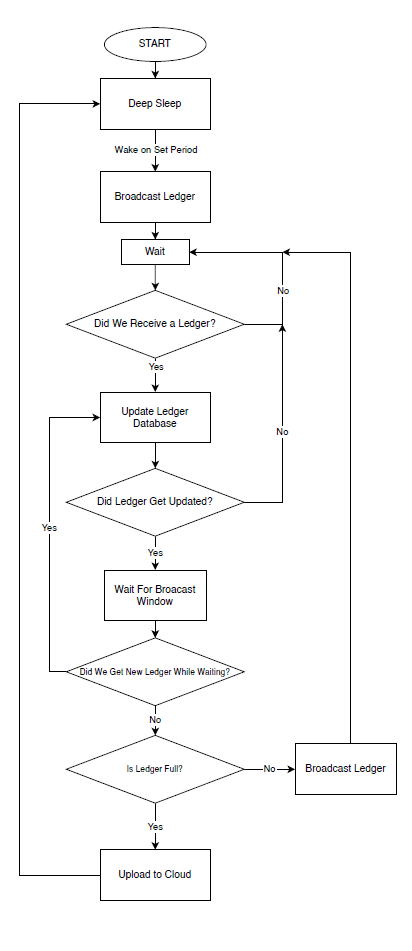
\includegraphics[width=1.41462in,height=3.26566in]{figs/method-image15.png}
\end{figure}

\subsubsection{Uploading the Data}

The cloud platform selected for this project is ThingSpeak.
To upload data, the base station performs an HTTP request using the
ThingSpeak API key. The request is sent using POST/GET (specify which
one is used). Upon successful upload, the server returns status code
\_\_\_.


Since the system can support up to 8 nodes, the base station
uploads each node's data individually using their respective API
keys.


\section{\texorpdfstring{Cloud}{Cloud}}

A cloud-based platform was required to allow researchers to access
sensor data remotely, as the turf houses are located far from the
research facilities and frequent on-site visits are impractical. Storing
data in the cloud enables continuous monitoring and simplifies data
access, making it easier for researchers to view and analyze
measurements without physically retrieving the devices.

Several criteria were considered when selecting a suitable cloud
platform. These included reliability, accessibility, low cost, ease of
integration with embedded systems, and the ability to store and
visualize time-series sensor data. While more advanced platforms such as
AWS or Microsoft Azure provide robust infrastructure, they were
considered unnecessarily complex and costly for the scope of this
project.

Based on these criteria, ThingSpeak was selected as the cloud platform.
ThingSpeak provides reliable data storage and built-in visualization
tools that are well suited for IoT applications. Given the expected data
transmission rate of the system, the required storage and upload
frequency fall within the limits of the free service tier, making it a
cost-effective solution. In this implementation, sensor data uploaded to
the cloud is stored and made readily accessible for remote viewing and
further analysis by researchers.

\section{Testing}

During the development of the project, multiple tests were conducted to
evaluate system performance and reliability. These tests included power
consumption measurements, LoRa range testing, and several preliminary
tests carried out at Háskóli Íslands prior to the final deployment. The
testing phase provided valuable insights into early system limitations
and failures, allowing necessary modifications and improvements to be
made before final deployment.

\subsection{In Situ Sensor Node Power Consumption
Tests}

After the initial assembly of a functional sensor node, power
consumption testing was conducted using a precision laboratory power
supply (Rohde \& Schwarz HMP2030), capable of measuring current down to
100 µA. The sensor module was powered at 4.2 V to represent a fully
charged battery condition, and the power supply's current readout was
used to observe and record current consumption.

During testing, the sensor node was programmed to cycle through multiple
operating states in a continuous loop. Each state was maintained for 10
seconds before transitioning to the next state, allowing the current
readings to stabilize. State transitions were controlled entirely
through firmware to ensure consistent and repeatable behavior. The
measurement cycle was allowed to run continuously, and power consumption
was observed over three complete loops to verify repeatability.

The operating states tested included the following:

\begin{itemize}
\item
  \textbf{Deep sleep mode}
\item
  \textbf{Awake mode with sensors enabled}
\item
  \textbf{LoRa transmission and reception mode}
\item
  \textbf{Half-sleep mode}, in which the sensor modules were
  disconnected while the LoRa module remained fully powered and the MCU
  in a light sleep mode.
\end{itemize}

\textbf{Deep Sleep Mode:}

Deep sleep mode completely shuts down most of the node's hardware
components to minimize power consumption for long-term operation. In
this mode, the system disables communication interfaces such as SPI and
I²C, turns off GPIO modules and the LoRa radio, and sets all pins to a
low-power state. Interrupts from the LoRa module are removed, and only
the real-time clock (RTC) interrupt is enabled to wake the device at
scheduled intervals. The microcontroller then enters the gotosleep()
state where almost all processes are halted. When the RTC interrupt
occurs, the system wakes up, re-enables the LoRa interrupt, powers the
modules back on, and reinitializes the LoRa configuration before
resuming normal operation. This mode is designed to achieve maximum
energy savings for battery-powered wireless sensor nodes that operate
for long periods between transmissions.

\textbf{Light Sleep Mode:}

Light sleep mode reduces power consumption while still keeping certain
communication capabilities active, particularly the LoRa module for
receiving data. In this mode, only non-essential devices and GPIO
modules are powered down, while LoRa is kept in receive mode so the node
can wake immediately when a packet arrives. The I²C communication is
disabled and unused pins are set to low-power states, but the system
maintains the LoRa interrupt to trigger wake-up. When the interrupt from
the LoRa module is detected, the microcontroller exits the sleep state
and resumes execution. Compared to deep sleep, light sleep consumes more
power but allows faster response times and continuous listening for
incoming LoRa messages, making it suitable for nodes that must remain
partially active within the wireless sensor network.

\subsection{Háskóli Íslands Preliminary Tests
1}

After all system components had been assembled and verified, an initial
set of local preliminary tests was conducted at Háskóli Íslands. With
permission from \textbf{{[}NAME TO BE UPDATED{]}} and Dorotea, testing
was carried out on the turf roofs located within the university campus.

A single LoRa base station was installed in Helgi's office, where it was
connected to a computer configured for continuous monitoring of incoming
data via the cloud platform. This setup allowed real-time observation of
device status, packet reception, and data integrity throughout the test
period.

Four sensor devices were deployed across the surrounding area, primarily
in the vicinity of the VR-II and VR-III buildings. All devices were
positioned within an approximate radius of 100 meters from the base
station, ensuring stable connectivity while enabling early validation of
system reliability under realistic deployment conditions. For this test,
each sensor was powered by a single battery cell in order to evaluate
power consumption and determine the operational lifetime achievable with
one cell.

The preliminary test phase was conducted over a three-week period, from
\textbf{June 8 to June 29, 2025}. During this time, the system operated
continuously, providing insight into long-term stability, data
consistency, and potential environmental effects on communication
performance.

\subsection{LoRa Range Tests}

Based on insights gained from the initial field tests, it became
necessary to conduct more extensive range testing to further evaluate
system performance under different conditions. Multiple LoRa
configurations were evaluated to determine the most optimal balance
between communication range and performance. Previous studies have
demonstrated that LoRa is capable of achieving significant transmission
distances under suitable conditions, and these claims needed to be
validated using the current hardware setup and deployment environment.

The LoRa transceiver supports a wide range of configurable parameters,
including operating frequency, transmission power, bandwidth, sync word,
spreading factor, coding rate, and preamble length. For these
experiments, several of these parameters were kept constant---namely
frequency, transmission power, sync word, coding rate, and preamble
length---in order to ensure fair and repeatable comparisons between
tests. The parameters that were primarily adjusted during testing were
bandwidth and spreading factor, as these have the most direct and
significant impact on range, data rate, and signal robustness.

\textbf{Key LoRa configuration parameters:}

\begin{itemize}
\item
  \textbf{Bandwidth (BW):} Determines the width of the frequency band
  used for transmission. Lower bandwidth improves receiver sensitivity
  and increases range, but reduces data rate.
\item
  \textbf{Spreading Factor (SF):} Controls how many chirps are used to
  encode each symbol. Higher spreading factors increase range and
  resistance to noise at the cost of lower data rates and longer
  transmission times.
\item
  \textbf{Transmission Power:} Defines the output power of the radio.
  This was kept constant to comply with regulatory limits and to isolate
  the effects of BW and SF.
\item
  \textbf{Coding Rate (CR):} Adds forward error correction to improve
  data reliability. This was fixed to maintain consistent error
  correction across tests.
\item
  \textbf{Preamble Length:} Used for receiver synchronization. A fixed
  preamble ensured consistent packet detection behavior.
\end{itemize}

Bandwidth and spreading factor were the primary variables during testing
because together they directly influence link budget and receiver
sensitivity. Adjusting other parameters would either violate regulatory
constraints or introduce additional variables that make performance
comparisons less reliable. By focusing on BW and SF, it was possible to
observe clear trade-offs between range, signal quality, and data
throughput.

The range tests were conducted in Vellir, located in Hafnarfjörður. The
base station was mounted on a fence at approximately chest height to
simulate a realistic low-elevation deployment. A mobile sensor node was
placed inside a vehicle and connected to a laptop for real-time
monitoring.

During the tests, the vehicle was driven around the surrounding area
while the base station transmitted randomly encoded data packets once
per second. The received signal strength indicator (RSSI) values were
recorded continuously, and received packets were inspected to verify
data integrity and detect any corruption. This approach allowed both
communication reliability and signal strength to be evaluated
simultaneously under real-world conditions.

\subsection{Háskóli Íslands Preliminary Tests
2}

Building on the insights gained from the previous preliminary tests and
subsequent system improvements, a longer-duration local test was
conducted at Háskóli Íslands. Due to seasonal conditions approaching
winter, access to the turf roofs was no longer permitted, as they were
required for ongoing studies by the responsible staff member.

As a result, four sensor devices were redeployed across the campus
within an approximate radius of 100 meters from the base station, using
the same monitoring and data collection setup as in the earlier tests.
The base station remained connected to a dedicated computer for
continuous cloud-based data monitoring. In this test, each sensor was
powered by a single battery cell, consistent with the previous test
configuration.

For this test phase, the antenna system was upgraded to improve
communication performance. Larger and higher-quality antennas were
installed on the sensor nodes, and an outdoor antenna was mounted
outside Helgi's office to enhance base station reception and
transmission.

This second preliminary test was conducted over an extended period, from
\textbf{August 1 to October 6, 2025}, allowing for evaluation of
long-term system stability, communication reliability, and the impact of
environmental conditions on performance.

\section{Deployment in Keldur}

After incorporating lessons learned from the previous test phases, the
system was considered ready for full deployment. In collaboration with
Dorotea, a deployment visit was arranged to \textbf{Keldur} (additional
site information to be added).

For this deployment, each sensor node was configured with the maximum
number of battery cells supported by the enclosure, which was three
cells per sensor. All sensors were fully sealed and prepared for
long-term outdoor operation prior to deployment.

Upon arrival at Keldur, the network infrastructure was already in place
from earlier testing. The Wi-Fi router was located in the attic of one
of the turf houses. The LoRa base station was installed at this location
and connected to the existing network, allowing immediate communication
with the cloud platform. Once verified, the base station equipment was
discreetly concealed to avoid visual impact, as the site operates as a
museum.

Following the base station setup, four sensor units were installed
around the area, with one sensor assigned to each turf roof.

\emph{{[}Further details describing sensor placement, mounting method,
and orientation to be added here, along with reference to deployment
photographs.{]}}

After installation, all equipment was confirmed to be operational and
securely concealed. The long-term deployment test commenced on
\textbf{October 17, 2025}, and is currently ongoing \textbf{{[}end date
to be updated upon completion{]}}.

\section{Calibration Method}

To determine the accuracy of the off-the-shelf soil moisture sensors
relative to an industry-standard instrument, the sensors were compared
side by side with a HOBO MX230x Soil Moisture and Temperature Data
Logger. The HOBO device is a fully integrated soil moisture logger with
Bluetooth-based wireless data offload capability and measures both soil
moisture and temperature.

To ensure scientific accuracy, the gravimetric method was performed
alongside the sensor comparison to establish the actual soil moisture
content. Calibration was conducted at {[}insert laboratory name{]}
located at VR-3.

An Icelandic soil sample was collected and oven-dried at 105 °C for 32
hours (from 11:00 AM to 8:00 PM the following day) to remove all
moisture and establish a dry baseline condition. After drying, the soil
was allowed to cool to room temperature before testing. A measured
portion of the dried soil was then placed in a container, and all
sensors were installed side by side to ensure identical environmental
conditions.

Water was added incrementally in 10\% increments relative to the dry
soil weight. A spray mister was used to distribute water evenly
throughout the soil. After each increment, sufficient time was allowed
for uniform saturation before measurements were recorded. At each
moisture level, multiple readings were collected from all sensors to
ensure consistency and reduce variability. This procedure was repeated
for each incremental moisture level.

The HOBO sensor provides measurements of volumetric water content (VWC)
in mineral soils, with a specified measurement range of 0.00 to 0.64
m³/m³. In this experiment, mineral soil configuration was used. Although
the device also allows alternative output settings, the selected
configuration was kept consistent throughout the experiment. Where
necessary, conversion equations were applied during data analysis to
ensure comparability of results.

The experiment continued until the soil reached full saturation and
additional water resulted in surface pooling, indicating that no further
absorption could occur. At this point, the calibration process was
concluded and all measurements were recorded and stored for analysis.

To ensure reliability and repeatability, the entire calibration
procedure was conducted twice. The first experiment was performed on
November 8, and the second on December 16.

\textbf{3.8.1 Reference Instrument: HOBO MX230x Soil Moisture and
Temperature Data Logger}

The HOBO MX230x Soil Moisture and Temperature Data Logger was used as
the reference instrument for calibration. This commercial device is
widely used in environmental monitoring studies and is also currently
utilized by research teams working on Icelandic turf roof monitoring.
Using this instrument as the reference ensures consistency and
comparability with existing research efforts.

The soil moisture sensor measures volumetric water content (VWC) with a
measurement range of 0.00 to 0.64 m³/m³ in mineral soils and 0.00 to
0.70 m³/m³ in soilless media. The typical accuracy is ±0.031 m³/m³ in
mineral soils (solution EC \textless{} 8 dS/m), with a resolution of
0.001 m³/m³. The sensor operates at a dielectric measurement frequency
of 70 MHz.

The integrated temperature sensor (MX2307) has a measurement range of
−40 °C to 100 °C with an accuracy of ±0.2 °C to ±0.25 °C depending on
the temperature range, and a resolution of 0.04 °C. The logger supports
adjustable logging intervals from 1 second to 18 hours and can store up
to 110,000 measurements. The device uses Bluetooth Low Energy for
wireless data retrieval and is powered by a 3.6 V lithium battery with a
typical operational life of up to several years, depending on logging
configuration.

The manufacturer also specifies that the soil moisture measurements can
be post-calibrated using custom calibration equations if higher accuracy
is required or if soil conditions differ from standard mineral soils.
This feature further supports its suitability as a calibration reference
instrument for this study.


\chapter{Results and Discussion}\label{chap:results}
\section{Overview}

\draftchange{This chapter presents the results obtained from laboratory power consumption testing, preliminary field trials at Háskóli Íslands, LoRa range evaluation, long-term deployment in Keldur, and soil moisture calibration. The results are analyzed in relation to the system requirements defined in Chapter 3, particularly long-term low-power operation, communication performance of the installed sensor nodes, mesh network operation, and calibration accuracy. The Keldur deployment demonstrated the system under real outdoor conditions, while the calibration tests characterized the response of the soil moisture sensor over the tested 0--40\% range using a calibration soil sample.}

\section{Power Consumption
Results}

\subsection{Packet Sending Time
Calculation}

The in situ sensor node operates under a strict duty cycle constraint,
remaining active for a maximum of 5 minutes per hour while spending the
remaining 55 minutes in deep sleep. The transition from deep sleep to
full operation, including sensor activation via MOSFET, data
acquisition, and shutdown, takes approximately 3.1 seconds.

LoRa packet airtime is determined by the sum of preamble and payload
durations:

\begin{equation}
T_{packet} = T_{preamble} + T_{payload}
\label{eq:packet-airtime}
\end{equation}

With spreading factor \(SF = 10\), bandwidth
\(BW = 125\text{ }\text{kHz}\), and preamble length
\(N_{preamble} = 8\), the symbol time is:

\begin{equation}
T_{sym} = \frac{2^{SF}}{BW} = \frac{2^{10}}{125000} = 0.008192\text{ }\text{s}
\label{eq:symbol-time}
\end{equation}

The preamble duration is therefore:

\begin{equation}
T_{preamble} = (N_{preamble} + 4.25) \cdot T_{sym} \approx 0.1\text{ }\text{s}
\label{eq:preamble-duration}
\end{equation}

The payload duration depends on the payload size \(PL\) \draftchange{and} is given by:

\begin{equation}
T_{payload} = N_{payload} \cdot T_{sym}
\label{eq:payload-duration}
\end{equation}

For the selected configuration (CRC enabled, explicit header, low data
rate optimization, coding rate 4/5), this simplifies to:

\begin{equation}
N_{payload} = 8 + 5 \cdot \left\lceil \frac{8PL + 4}{32} \right\rceil
\label{eq:payload-symbols}
\end{equation}

Thus, total packet airtime becomes:

\begin{equation}
T_{packet} = \left( 20.25 + 5 \cdot \left\lceil \frac{8PL + 4}{32} \right\rceil \right) \cdot 0.008192
\label{eq:total-packet-airtime}
\end{equation}

For a 96-byte payload, the airtime is approximately 1.19 seconds per
transmission.

Assuming six sensor data types (e.g., temperature, humidity, soil
temperature, battery level, and timestamp) are transmitted eight times
per hour, the total transmission time is:

\begin{equation}
(1.19\text{ }\text{s} \times 8) \times 6 \approx 57\text{ }\text{s}
\label{eq:hourly-transmission-time}
\end{equation}

This is approximated to 1 minute of transmission time per hour. Then we
can assume that the rest is spent receiving LoRa packets and operating
in standby mode, which is approximately 237 seconds.

\clearpage
\subsection{Operating Modes}

\begin{longtable}[]{@{}
  >{\raggedright\arraybackslash}p{(\columnwidth - 6\tabcolsep) * \real{0.2457}}
  >{\raggedright\arraybackslash}p{(\columnwidth - 6\tabcolsep) * \real{0.2026}}
  >{\raggedright\arraybackslash}p{(\columnwidth - 6\tabcolsep) * \real{0.1634}}
  >{\raggedright\arraybackslash}p{(\columnwidth - 6\tabcolsep) * \real{0.3884}}@{}}
\caption{Operating states, measured current consumption, and duration per hour.}
\label{tab:operating-modes}\\
\toprule\noalign{}
\begin{minipage}[b]{\linewidth}\raggedright
\textbf{Operating State}
\end{minipage} & \begin{minipage}[b]{\linewidth}\raggedright
\textbf{Measured Current (mA)}
\end{minipage} & \begin{minipage}[b]{\linewidth}\raggedright
\textbf{Duration per Hour}
\end{minipage} & \begin{minipage}[b]{\linewidth}\raggedright
\textbf{Notes}
\end{minipage} \\
\midrule\noalign{}
\endfirsthead
\endhead
\bottomrule\noalign{}
\endlastfoot
Deep Sleep & 0.3 mA & 55 minutes & All modules off, MCU in deep sleep \\
Awake (Sensors ON / LoRa OFF) & 9.5 mA & 3 s & Sensor initialization and
data acquisition \\
LoRa RX/TX & 119.5 mA & 60 s & Transmission and reception of LoRa
packets \\
Half Sleep & 12.2 mA & 237 s & Sensors off, MCU in low-power mode, LoRa
in standby \\
\end{longtable}

\draftchange{During the laboratory test described in Section~\ref{sec:power-tests}, each operating state was maintained for 10 seconds to allow the current reading to stabilize. The measurement routine was observed over three complete loops to verify repeatability. The durations per hour shown in Table~\ref{tab:operating-modes} represent the operating-cycle durations used for the weighted average current calculation; they were not the duration of the laboratory measurement itself. Therefore, the average current consumption of approximately 3.08 mA is a calculated hourly cycle average based on the measured current in each operating state and its corresponding operating duration, rather than a direct average-current measurement taken over a continuous one-hour test.}

The average current consumption is calculated as:

\begin{equation}
I_{avg} = \frac{\sum I_{n}t_{n}}{T}
\label{eq:average-current}
\end{equation}

where \(I_{n}\) \draftchange{is} the current in each state, \(t_{n}\) \draftchange{is} the duration of
each state, and \(T = 3600\text{ }\text{s}\) \draftchange{is} the total time per hour.

Substituting the measured values:

\begin{equation}
\begin{aligned}
I_{avg} &=
\frac{(0.3 \times 3300) + (9.5 \times 3) + (119.5 \times 60)
+ (12.2 \times 237)}{3600} \\
&= \frac{990 + 28.5 + 7170 + 2891.4}{3600} \\
&\approx 3.08\,\text{mA}
\end{aligned}
\label{eq:average-current-substitution}
\end{equation}

Thus, the average current consumption of the sensor node under
worst-case conditions is approximately \textbf{3.08 mA}.

Given a total battery capacity of 10,500 mAh (three 3,500 mAh cells in
parallel), the estimated operational lifetime is:

\begin{equation}
\frac{10500}{3.08} \approx 3409\text{~hours} \approx 142\text{~days~}( \sim 4.7\text{~months})
\label{eq:three-cell-lifetime}
\end{equation}

This estimate assumes ideal battery performance. In practice,
environmental factors---particularly low temperatures in Iceland---will
reduce effective battery capacity and shorten the operational lifetime.

For comparison, a single 3,500 mAh cell would yield an estimated
lifetime of approximately:

\begin{equation}
\frac{3500}{3.08} \approx 1136\text{~hours} \approx 47\text{~days}
\label{eq:single-cell-lifetime}
\end{equation}

This highlights the importance of parallel battery configuration for
extended deployment.

\draftchange{Overall, the estimated operating lifetime is considered sufficient for the intended application.} Turf roofs are periodically inspected and maintained,
allowing battery replacement to be integrated into routine maintenance
cycles. This ensures continuous operation of the sensor nodes while
supporting long-term monitoring of soil conditions and turf roof
integrity.

\section{Initial Field
Deployment}

\draftchange{An initial field test was conducted on the University of Iceland (Háskóli Íslands) campus, with sensor nodes positioned approximately 50--100 m from the base station.} The primary objective of
this deployment was not to evaluate the final performance of the system,
but rather to validate the functionality of the preliminary hardware,
firmware, and communication system under real outdoor conditions. Since
turf roofs are present at several buildings on campus, including the
turf-covered bicycle shed, these locations provided an accessible
environment for testing while allowing rapid troubleshooting and
hardware modifications during development.

Four prototype sensor nodes (HW\_1, HW\_3, HW\_5, and HW\_7) were
deployed to collect air temperature, relative humidity, soil
temperature, and soil moisture data. Measurements were transmitted
through the LoRa network to the base station and uploaded to the cloud
for analysis. \draftchange{Measurements from the prototype sensor nodes were cross-checked against observations from the Reykjavík Hljómskálagarður automatic weather station (Station 1469), operated by Veðurstofa Íslands~\cite{imo_observations}.}

\subsection{Air Temperature and Relative
Humidity}

Figure~\ref{fig:results-1} compares the measured air temperature from the prototype
sensor nodes with the \draftchange{Reykjavík Hljómskálagarður weather station (Station 1469)}, while Figure~\ref{fig:results-2} presents
the corresponding relative humidity measurements.

\begin{figure}[htbp]
\centering
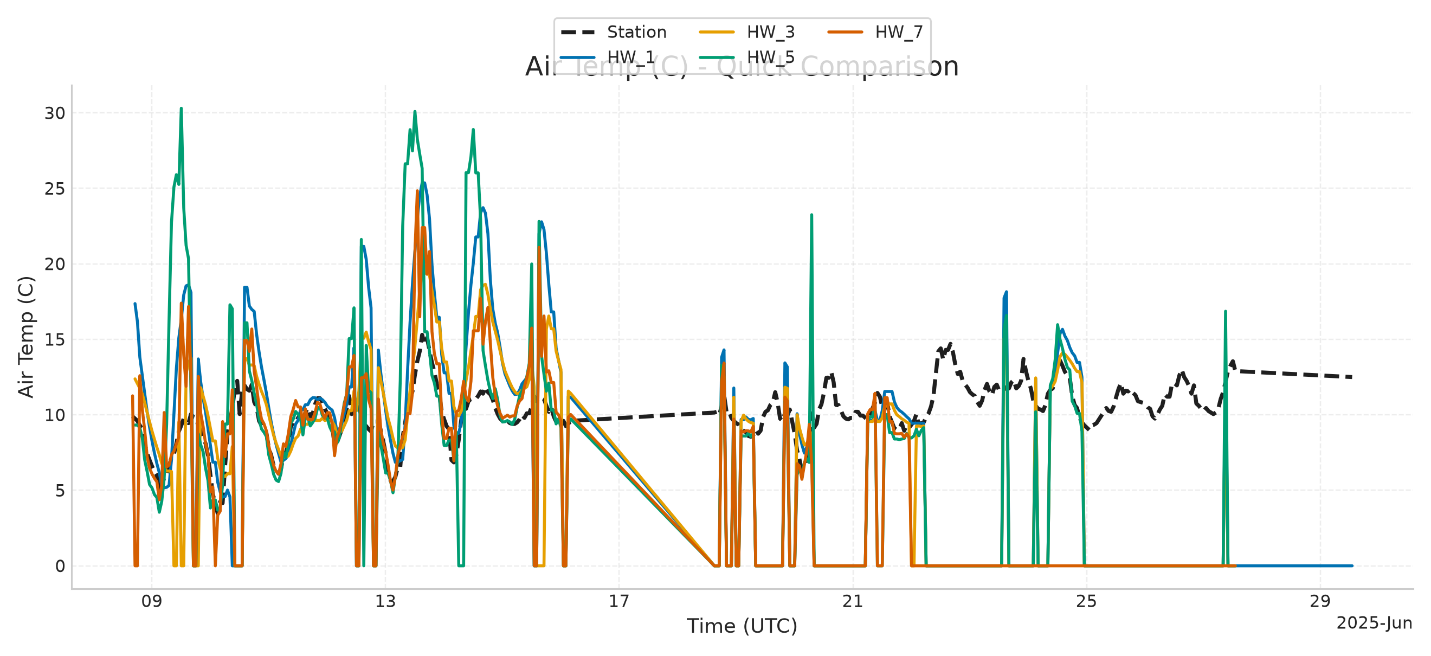
\includegraphics[width=\textwidth,height=2.97917in,keepaspectratio]{figs/results-image1.png}
\caption{Air temperature measurements during the preliminary field deployment.}
\label{fig:results-1}
\end{figure}

\begin{figure}[htbp]
\centering
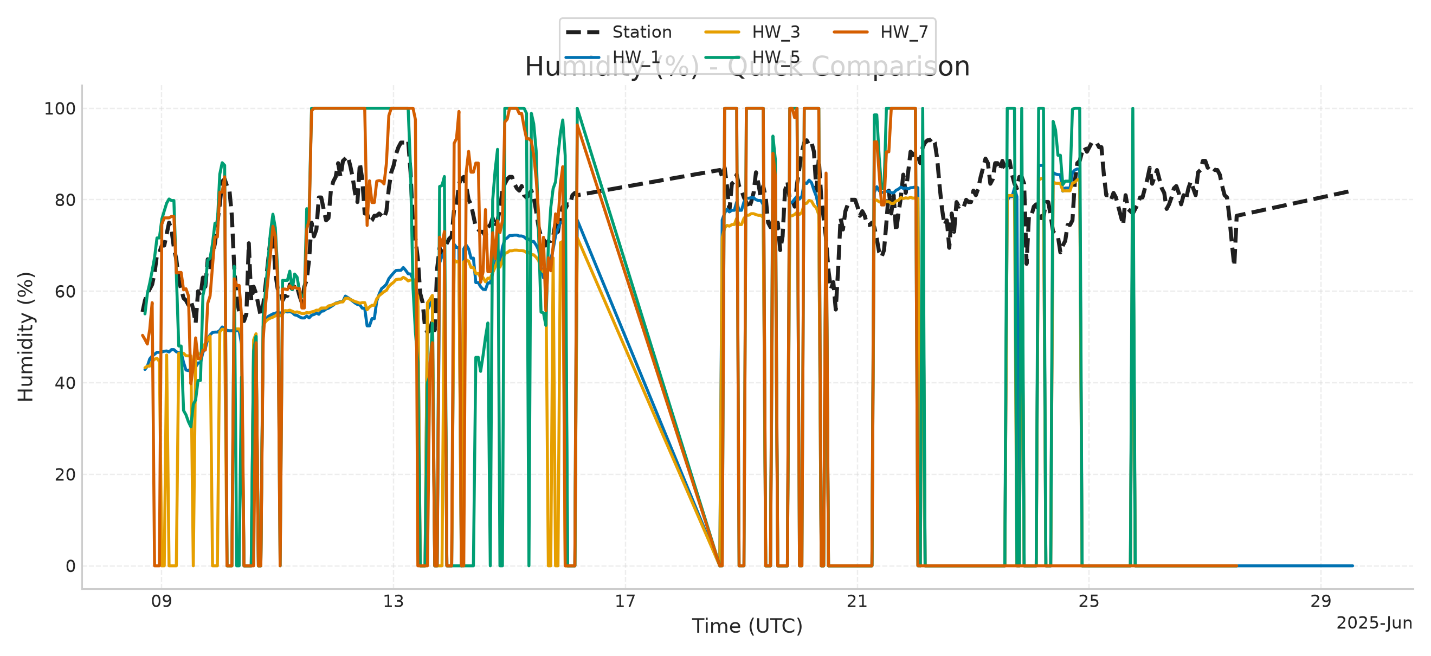
\includegraphics[width=\textwidth,height=2.97917in,keepaspectratio]{figs/results-image2.png}
\caption{Relative humidity measurements during the preliminary field deployment.}
\label{fig:results-2}
\end{figure}

The prototype nodes successfully collected environmental measurements
throughout the deployment period and generally followed the overall
trends observed by the weather station. However, numerous interruptions,
missing samples, and unstable readings were observed. These
inconsistencies were expected because the firmware and hardware were
still under active development, with frequent updates and adjustments
being performed throughout the testing period.

\draftchange{The comparison with the weather station was intended as a contextual cross-check of general environmental trends. It was not a direct calibration or an absolute accuracy validation, because the sensor nodes and the weather station were located at different sites.}

One of the major issues identified during this deployment was poor LoRa
communication performance. During testing, the sensor nodes were
initially equipped with commercially available antennas that were later
found to be designed primarily for Wi-Fi frequencies rather than the
\textbf{433 MHz LoRa frequency} used by the system. As a result, signal
quality was significantly degraded, leading to frequent packet loss,
communication interruptions, and incomplete datasets. This issue was
identified during the preliminary deployment and later resolved by
replacing the antennas with properly tuned 433 MHz LoRa antennas before
the final deployment.

\subsection{Soil Temperature and Soil
Moisture}

Figure~\ref{fig:results-3} presents the measured soil temperature, while Figure~\ref{fig:results-4}
shows the corresponding soil moisture measurements collected during the
preliminary deployment.

\begin{figure}[htbp]
\centering
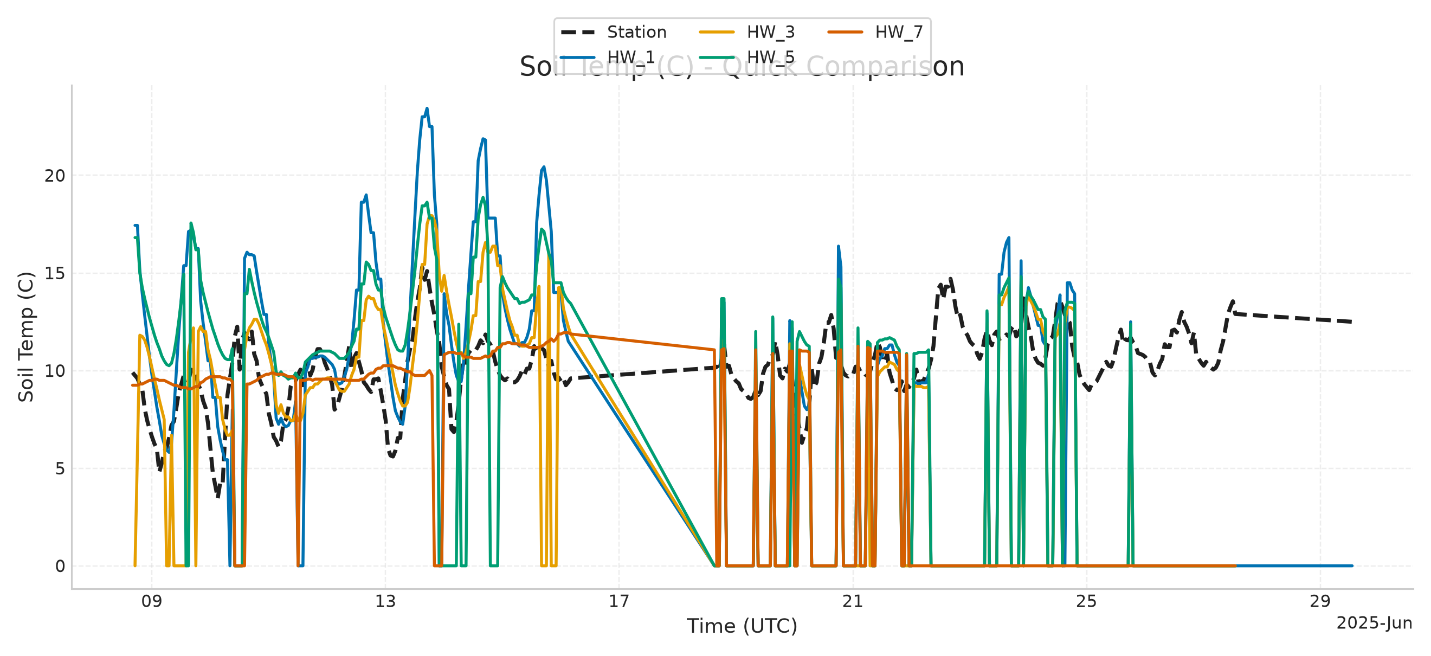
\includegraphics[width=\textwidth,height=2.97917in,keepaspectratio]{figs/results-image3.png}
\caption{Soil temperature measurements during the preliminary field deployment.}
\label{fig:results-3}
\end{figure}

\begin{figure}[htbp]
\centering
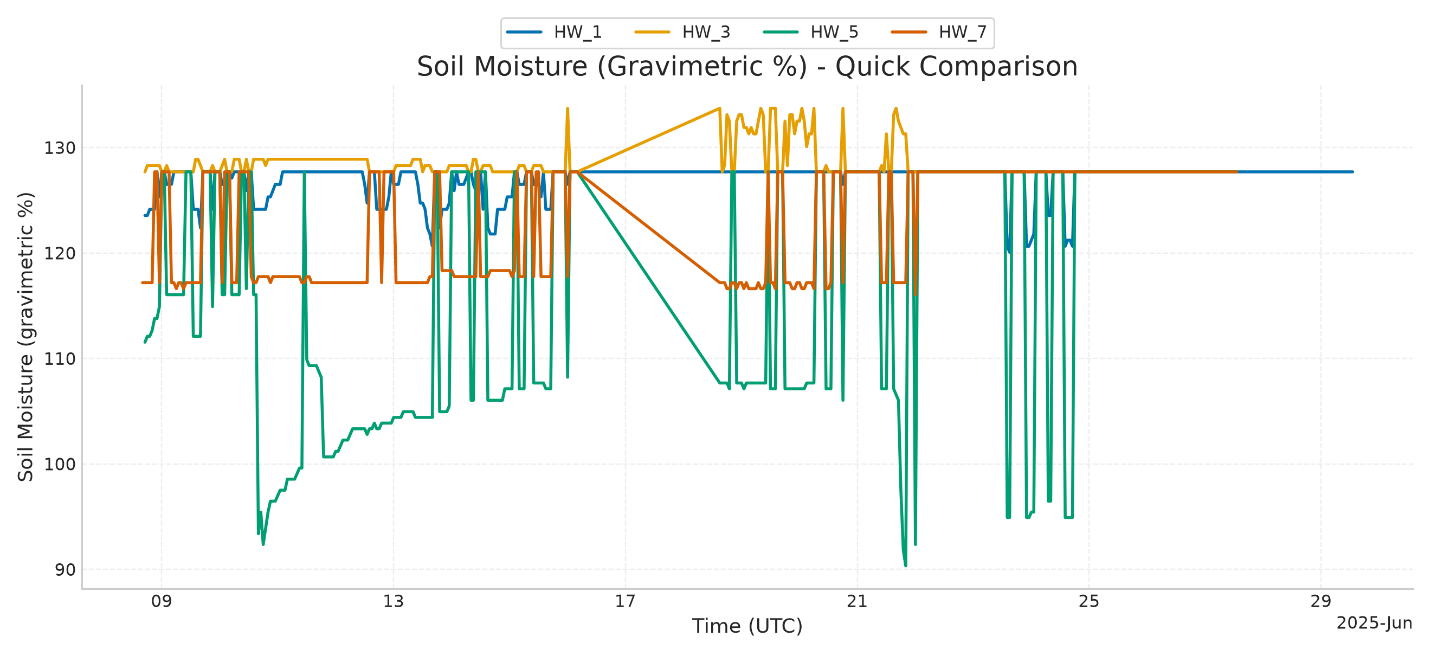
\includegraphics[width=\textwidth,height=2.97917in,keepaspectratio]{figs/results-image4.png}
\caption{Soil moisture measurements during the preliminary field deployment.}
\label{fig:results-4}
\end{figure}

The prototype sensor nodes successfully measured subsurface temperature
and soil moisture while installed beneath the turf roofs. Similar to the
later deployments, soil temperature exhibited considerably smaller
fluctuations than ambient air temperature due to the thermal buffering
properties of the surrounding soil.

The soil moisture measurements, however, showed considerable variability
and several unrealistic values exceeding the expected physical range. At
this stage of development, the moisture sensors had not yet undergone
final calibration, and firmware updates affecting sensor scaling were
still being tested. Combined with the communication issues caused by the
incorrect antennas, the resulting datasets contained numerous missing
samples and erroneous measurements. Nevertheless, the deployment
successfully demonstrated that the sensing hardware, analog measurement
circuitry, and cloud logging system operated correctly under outdoor
conditions.

\subsection{Summary of Preliminary
Testing}

The preliminary field deployment successfully fulfilled its intended
purpose as an engineering validation phase. Although the collected
environmental data were not suitable for scientific analysis due to
communication interruptions and ongoing hardware development, the
testing identified several important issues that were subsequently
corrected. Most notably, replacing the incorrectly matched antennas with
antennas specifically designed for the 433 MHz LoRa frequency
significantly improved communication reliability and packet delivery in
later deployments. Additional improvements included refinements to the
firmware, sensor calibration procedures, enclosure design, and overall
system stability.

\draftchange{Local SD card backup was implemented and tested. During the earlier testing, the measurements stored on the SD card were used to fill missing or blank values in the collected dataset where wireless transmissions had been missed. This showed that the local storage could be used to recover data that had not reached the base station during communication interruptions.}

The knowledge gained from this preliminary deployment formed the basis
for the final hardware revision used in the subsequent long-term field
deployment, where substantially improved communication reliability and
data quality were achieved.

\clearpage
\section{LoRa Range Testing Results (Vellir --
Hafnarfjörður)}\label{sec:lora_range_testing}

\subsection{Test Configurations}

The following configuration parameters were used during the LoRa field
range testing:

\begin{lstlisting}[
    caption={LoRa configuration parameters used during field range testing.},
    label={lst:lora-test-config},
    basicstyle=\normalsize\ttfamily,
    breaklines=true,
    captionpos=b,
    escapeinside={(*@}{@*)}
]
#define FREQUENCY       433E6   // 433 MHz
#define TX_POWER        17      // dBm
#define BANDWIDTH       125E3   // 125 kHz
#define SYNC_WORD       0x12
#define SPREAD_FACTOR   10
#define CODING_RATE     5
#define PREAMBLE        8
\end{lstlisting}

During the initial field test, communication performance was limited due
to the use of antennas designed for Wi-Fi rather than LoRa. These
antennas were not tuned for the 433 MHz operating frequency, resulting
in significantly reduced range. After replacing them with antennas
designed specifically for LoRa frequencies, a substantial improvement in
communication performance was observed.

Field testing was conducted in a semi-urban environment around Vellir in
Hafnarfjörður. Using the configuration described above, reliable
communication was achieved within an approximate radius of 3 km. Signal
quality improved when the transmitting node was positioned at elevated
locations, highlighting the importance of antenna placement.

In areas with dense infrastructure, such as residential zones with
multiple buildings obstructing the line of sight, signal degradation and
occasional packet loss were observed. This confirms that LoRa
performance is strongly influenced by environmental obstructions and
benefits from relatively clear propagation paths.

\begin{figure}[htbp]
\centering
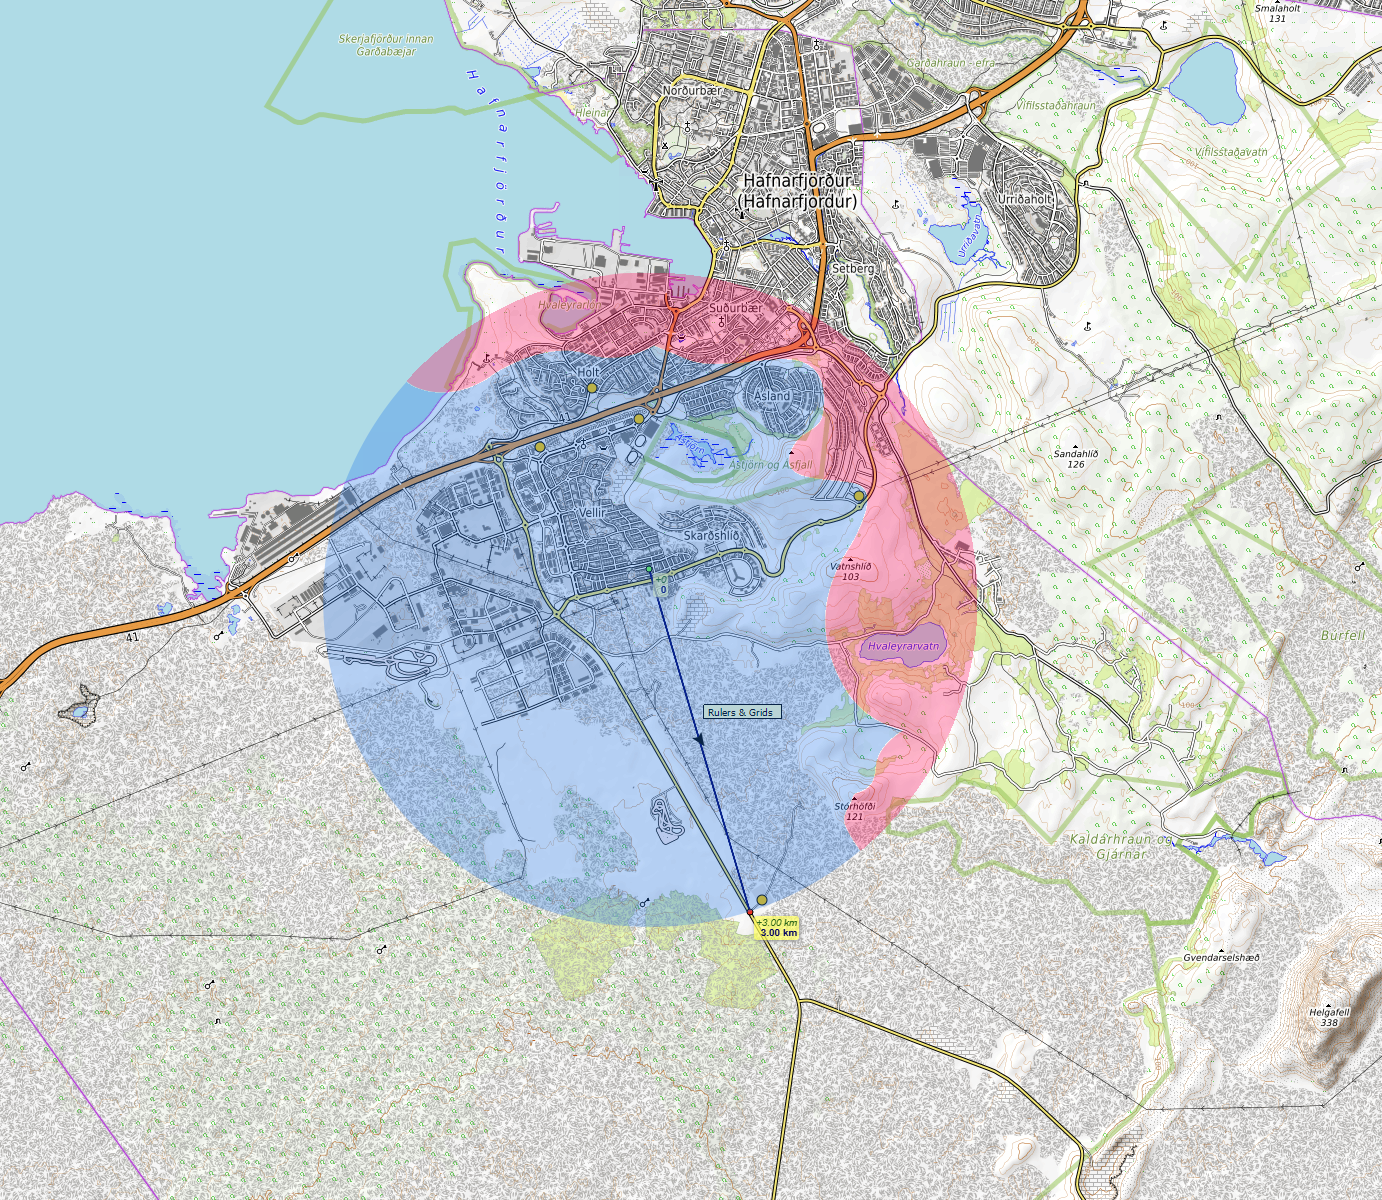
\includegraphics[width=\textwidth,height=5.64583in,keepaspectratio]{figs/results-image5.png}
\caption{Estimated LoRa signal coverage map for the Vellir--Hafnarfjörður field test. Blue regions indicate reliable communication coverage at approximately 3 km, while red regions indicate weak or absent signal strength due to terrain and structural obstructions.}
\label{fig:results-5}
\end{figure}

\draftchange{The estimated signal coverage map is shown in Figure~\ref{fig:results-5}.} Regions marked in red represent areas where no signal was
detected, primarily due to terrain obstructions such as hills and dense
built environments.

Signal strength measurements were recorded at multiple locations within
the testing area. The average RSSI values are summarized in the RSSI table.

\begin{table}[htbp]
\centering
\caption{Average RSSI values recorded at each test location during the LoRa range evaluation.}
\label{tab:rssi-summary}
\begin{tabular}{p{0.55\textwidth} p{0.25\textwidth}}
\toprule
\textbf{Location} & \textbf{Average RSSI} \\
\midrule
Ásvallalaug & -113 dBm \\
Holt & -103 dBm \\
Fish Drying Area & -112 dBm \\
Vatnslíð & -103 dBm \\
Netto & -112 dBm \\
\bottomrule
\end{tabular}
\end{table}

\subsection{Discussion of Results}

\draftchange{The results demonstrate reliable single-hop LoRa communication within an approximate 3 km radius. The recorded RSSI values, ranging from -103 dBm to -113 dBm, provide a useful indication of the communication performance achieved with the selected radio configuration and antennas.}

\draftchange{The Vellir range test evaluated direct, single-hop communication only; it did not evaluate the mesh relay process. A separate informal relay test was conducted during firmware development (Section~\ref{sec:informal-multihop}). Sensor nodes were spaced apart, and the researcher observed debug output showing ledger data being forwarded between nodes and eventually reaching the base station. Because this test was not logged and its topology, node count, spacing, and firmware revision were not retained, it provides qualitative evidence that the relay mechanism operated but does not provide measured multi-hop range, packet-delivery ratio, hop count, or latency. A controlled, logged multi-hop test is still needed to quantify those performance measures. Actual performance in turf-roof installations will also depend on antenna placement, burial depth, terrain, and surrounding structures.}

\section{Intermediate Field
Deployment}

Following the preliminary field testing, an intermediate field
deployment was conducted to evaluate the performance of the revised
hardware after replacing the original antennas with antennas
specifically designed for the \textbf{433 MHz LoRa operating frequency}.
The deployment was again carried out at several turf roof locations
around the \textbf{University of Iceland (Háskóli Íslands)} campus,
allowing rapid access to the sensor nodes for hardware modifications and
firmware updates while operating under real outdoor conditions.

The primary objective of this deployment was to verify the improvements
in LoRa communication reliability, evaluate the stability of the
environmental sensors, and identify any remaining hardware or software
issues before proceeding to the final long-term deployment. Four sensor
nodes (HW\_1, HW\_3, HW\_5, and HW\_7) continuously monitored air
temperature, relative humidity, soil temperature, and soil moisture,
while measurements from the \draftchange{Reykjavík Hljómskálagarður weather station (Station 1469) were used as a contextual cross-check.}

\subsection{Air Temperature and Relative
Humidity}

\draftchange{Figure~\ref{fig:results-6} compares the measured air temperature from the four prototype sensor nodes with the Reykjavík Hljómskálagarður weather station (Station 1469), while Figure~\ref{fig:results-7} presents the corresponding relative humidity measurements. As in the preliminary deployment, this comparison is a contextual cross-check of general trends rather than a calibration or absolute accuracy validation, because the instruments were located at different sites.}

\begin{figure}[htbp]
\centering
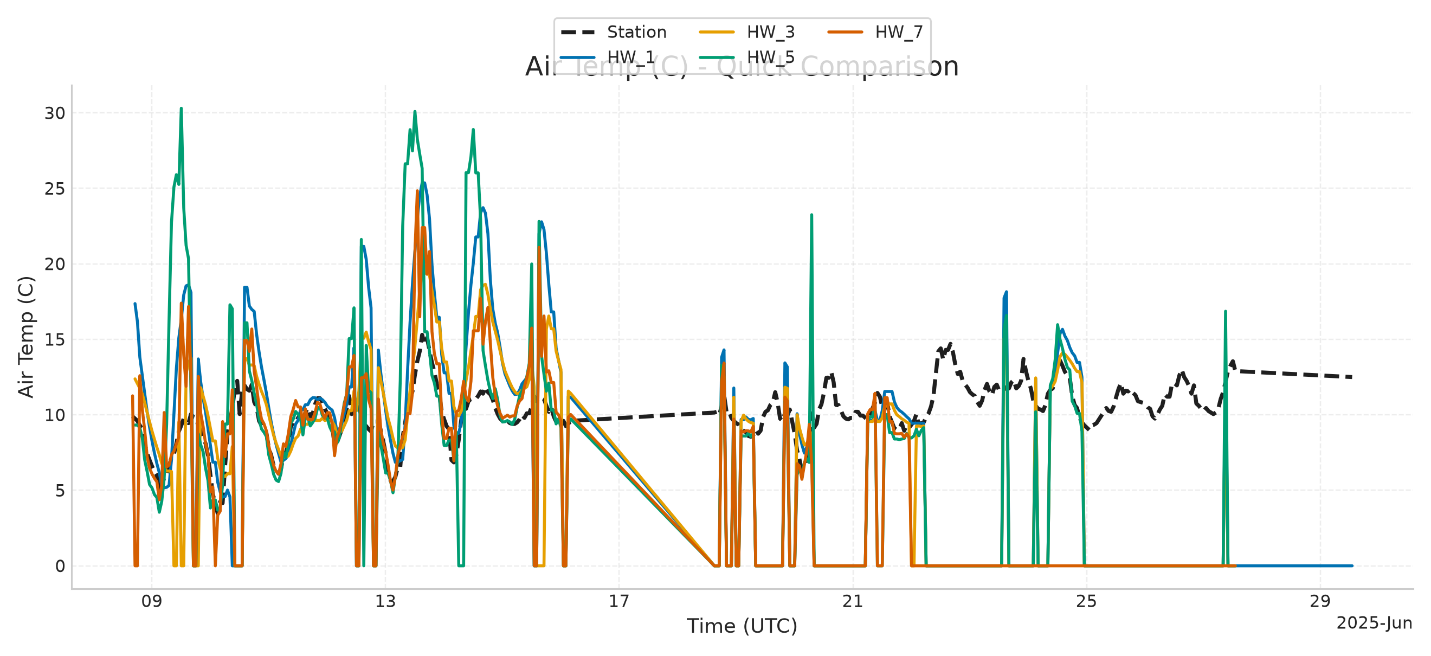
\includegraphics[width=\textwidth,height=2.97917in,keepaspectratio]{figs/results-image1.png}
\caption{Air temperature measurements during the intermediate field deployment.}
\label{fig:results-6}
\end{figure}

Compared with the preliminary deployment described in Section 4.3,
replacing the antennas with properly matched \textbf{433 MHz LoRa
antennas} resulted in a noticeable improvement in communication
reliability. Longer periods of uninterrupted environmental data were
successfully transmitted to the base station, reducing the amount of
missing data caused by packet loss.

The measured air temperatures generally followed the same trends as the
\draftchange{Reykjavík Hljómskálagarður weather station}, demonstrating that the revised communication
hardware allowed more consistent data collection. Relative humidity
measurements also became more stable; however, occasional readings of
\textbf{0\%} and \textbf{100\%} were still observed. These values were
attributed primarily to ongoing firmware development and sensor
initialization issues rather than communication failures. Since the
system remained under active development, firmware updates and hardware
adjustments continued throughout the testing period.

\begin{figure}[htbp]
\centering
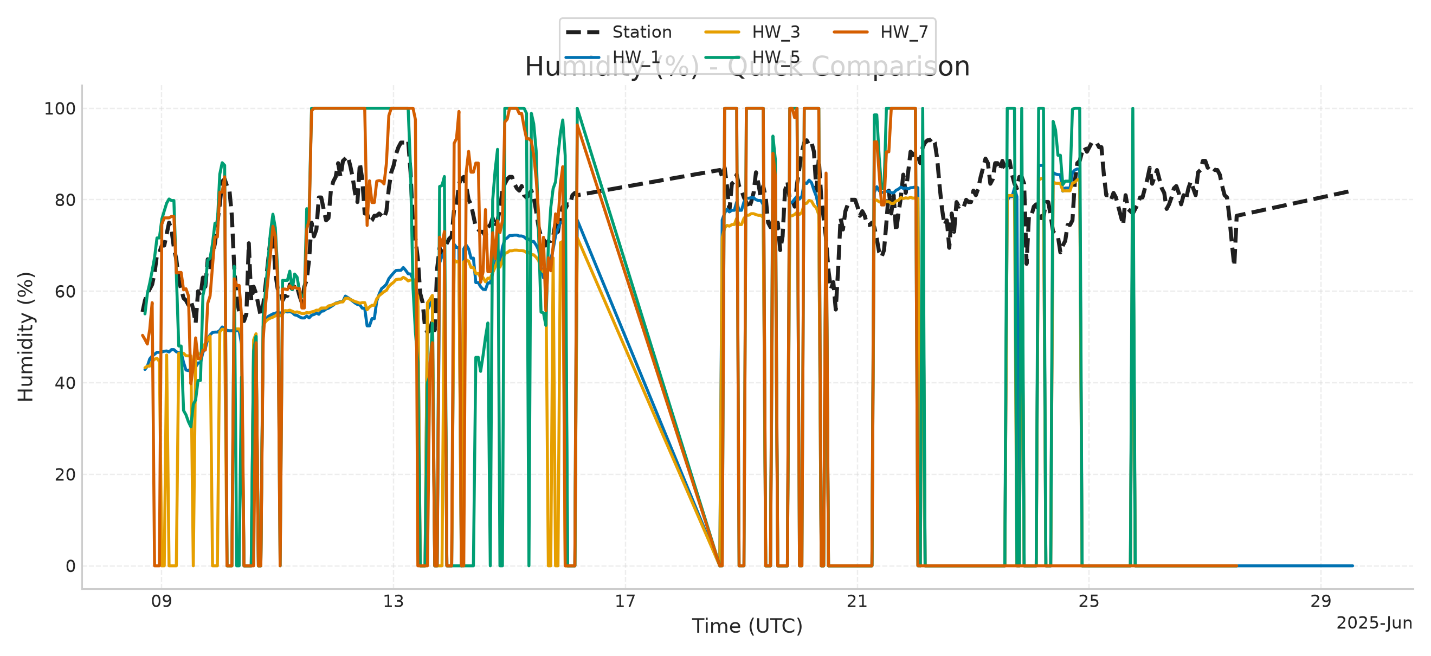
\includegraphics[width=\textwidth,height=2.97917in,keepaspectratio]{figs/results-image2.png}
\caption{Relative humidity measurements during the intermediate field deployment.}
\label{fig:results-7}
\end{figure}

\subsection{Soil Temperature and Soil
Moisture}

Figure~\ref{fig:results-10} presents the measured soil temperature from the deployed
sensor nodes, while Figure~\ref{fig:results-11} illustrates the corresponding soil
moisture measurements.

\begin{figure}[htbp]
\centering
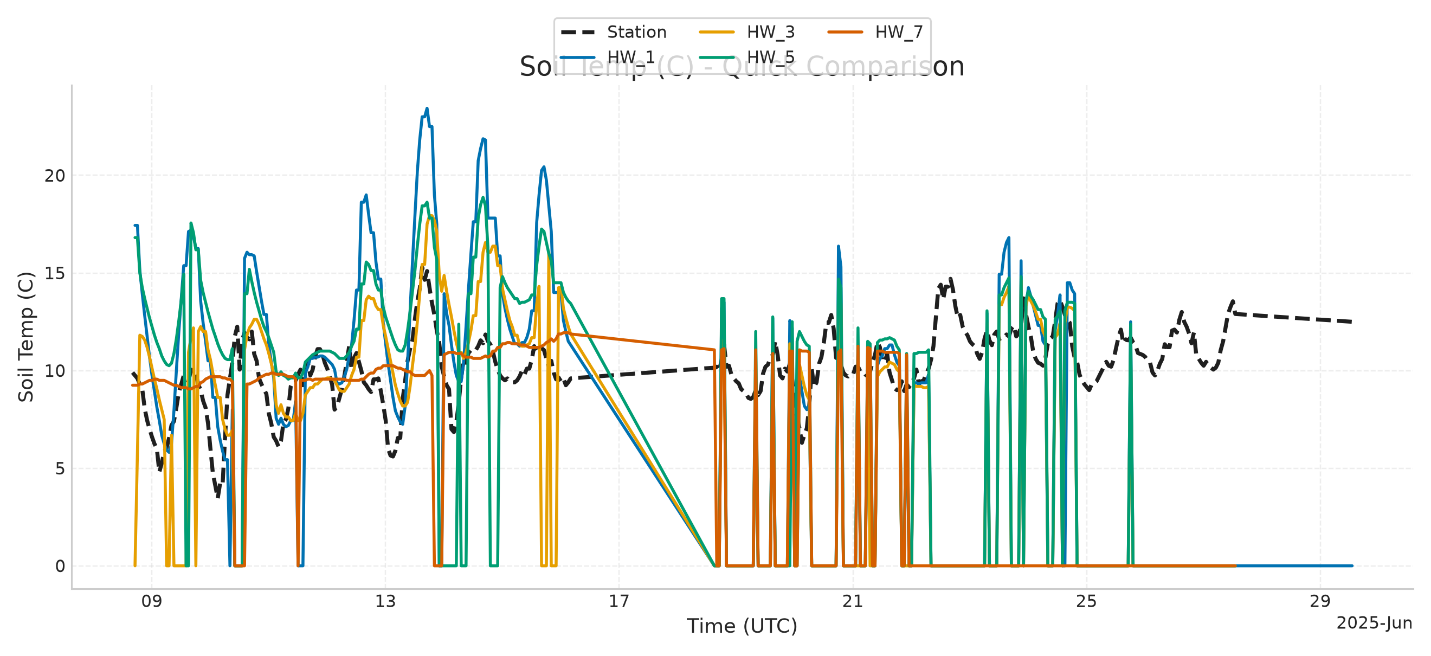
\includegraphics[width=\textwidth,height=2.97917in,keepaspectratio]{figs/results-image3.png}
\caption{Soil temperature measurements during the intermediate field deployment.}
\label{fig:results-10}
\end{figure}

Soil temperature measurements became more continuous than those obtained
during the preliminary deployment, reflecting the improved communication
performance achieved after replacing the antennas. The measured soil
temperatures remained more stable than ambient air temperatures,
demonstrating the thermal buffering effect of the surrounding soil.

\begin{figure}[htbp]
\centering
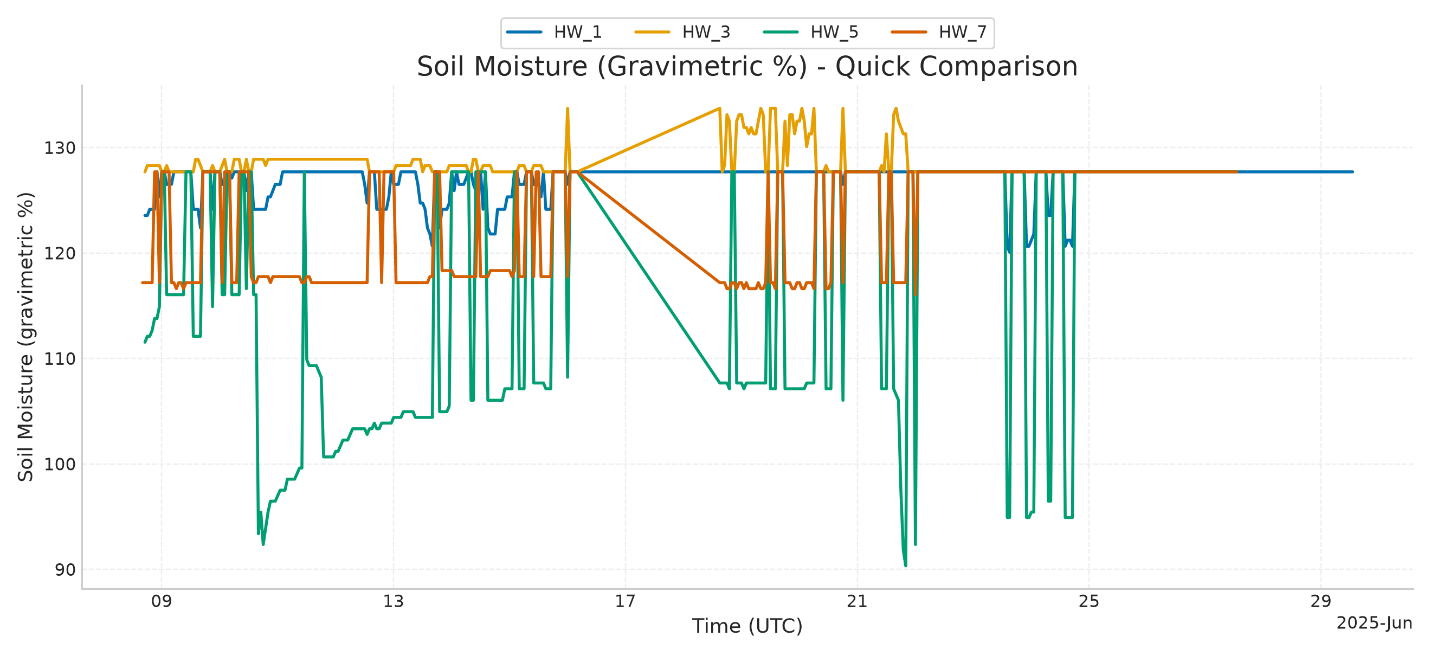
\includegraphics[width=\textwidth,height=2.97917in,keepaspectratio]{figs/results-image4.png}
\caption{Soil moisture measurements during the intermediate field deployment.}
\label{fig:results-11}
\end{figure}

The soil moisture measurements continued to exhibit considerable
variability because calibration procedures were still being refined.
Several nodes produced unrealistic values outside the expected
measurement range, indicating that further calibration and firmware
improvements were required before long-term deployment. Although these
measurements were not yet suitable for quantitative environmental
analysis, they confirmed that the sensing hardware, analog measurement
circuitry, and data logging system were operating correctly under
outdoor conditions.

\subsection{Summary}

The intermediate field deployment confirmed that replacing the original
antennas with antennas specifically designed for the \textbf{433 MHz
LoRa frequency} substantially improved wireless communication
reliability. Compared with the preliminary deployment, significantly
longer periods of continuous environmental data were successfully
collected, demonstrating that the antenna mismatch had been a major
contributor to the communication problems previously observed.

Although several issues related to firmware stability and sensor
calibration remained, the deployment successfully validated the revised
communication hardware and identified the final improvements required
before the long-term deployment. The experience gained during this stage
led to further refinements in the firmware, sensor calibration
procedures, and enclosure design, resulting in the final hardware
configuration used for the subsequent deployment at the Keldur turf
house site.

\section{Keldur Deployment}

To evaluate the performance of the proposed LoRa mesh wireless sensor
network under actual operating conditions, a field deployment was
conducted at the Keldur turf house site beginning on \textbf{17 October
2025}. Four sensor nodes (IDs 1, 3, 5, and 7) were installed at
different locations and depths beneath the turf roof. The installation
locations and sensor depths are shown in \draftchange{Figure~\ref{fig:results-deployment-map}}. Sensor Nodes
1 and 3 were designed with the air temperature and humidity sensors
enclosed inside the waterproof housing, while Sensor Nodes 5 and 7 had
these sensors mounted externally above the enclosure. This design
variation was intentionally implemented to compare the measurement
accuracy of both configurations under real environmental conditions.

\draftchange{Weather data used for comparison were obtained from the Sámsstaðir automatic weather station, operated by the Icelandic Meteorological Office (Veðurstofa Íslands), through the Icelandic Meteorological Office observation database~\cite{imo_observations}. It is commonly identified as \textit{samst}, station 6222, and has been active since 2000. It is the closest station listed on vedur.is to the Keldur test site, at a distance of 9.75 km. Its coordinates are latitude 63.735370636° and longitude -20.1090698242°.}

\clearpage
\begin{figure}[p]
    \centering
    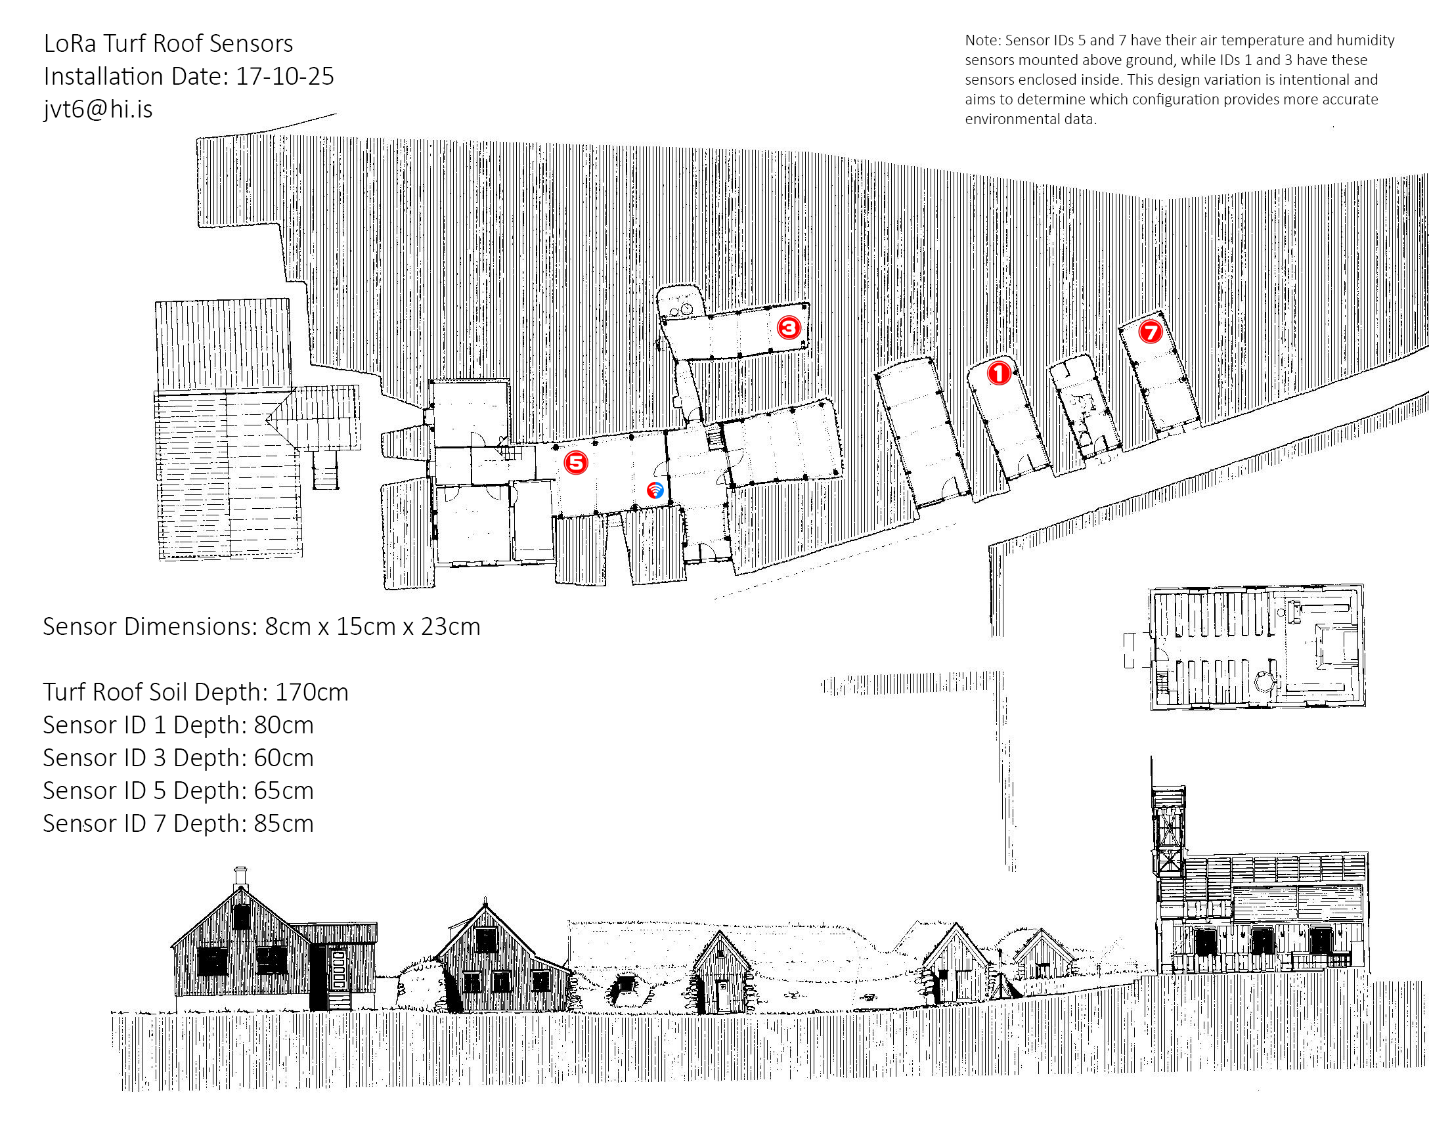
\includegraphics[
        angle=90,
        width=\textwidth,
        height=0.88\textheight,
        keepaspectratio
    ]{figs/results-image6.png}
    \caption{Deployment map showing the locations and installation depths of the four sensor nodes at the Keldur turf roof site.}
    \label{fig:results-deployment-map}
\end{figure}
\clearpage

\subsection{Air Temperature
Performance}

\draftchange{Figure~\ref{fig:results-12} compares the measured air temperature from all deployed sensor nodes with data obtained from the Sámsstaðir station (samst, 6222).}

\begin{figure}[htbp]
\centering
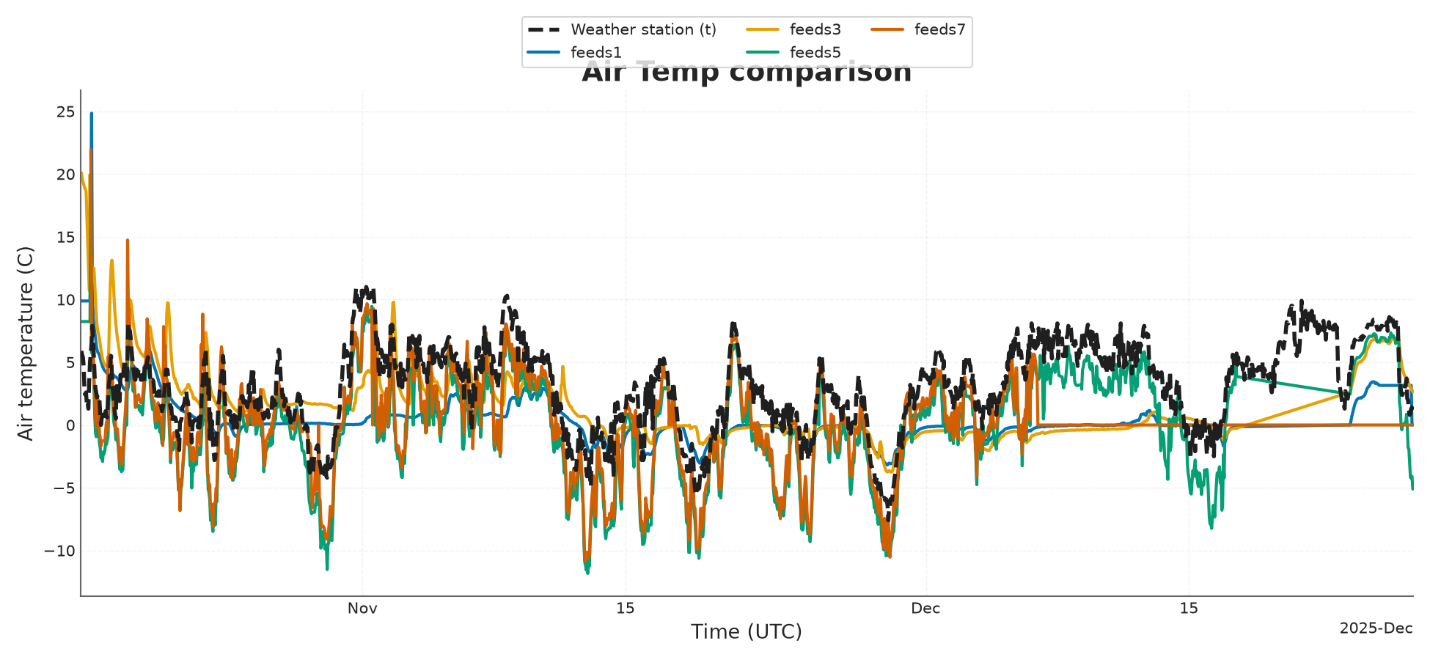
\includegraphics[width=\textwidth,height=3in,keepaspectratio]{figs/results-image7.png}
\caption{\draftchange{Comparison of air temperature measurements from the deployed sensor nodes and the Sámsstaðir station (samst, 6222).}}
\label{fig:results-12}
\end{figure}

\draftchange{The air temperature measurements from Sensor Nodes 5 and 7, which had externally mounted atmospheric sensors, generally followed the broader temperature variations observed at the Sámsstaðir weather station. Their measurements showed clearer daily fluctuations compared with Sensor Nodes 1 and 3, whose atmospheric sensors were installed inside the waterproof enclosure.}

\draftchange{The enclosed sensors produced smoother temperature curves with reduced daily variation. This suggests that placing the sensor inside the enclosure can affect how quickly it responds to changes in the surrounding air. The enclosure and its internal environment may contribute to this effect, although their individual influence was not measured separately.}

\draftchange{The average absolute temperature difference between the deployed sensors and station 6222 ranged from approximately \textbf{3.06 °C to 3.27 °C}. These values should be interpreted as differences between two measurement locations rather than direct sensor accuracy measurements. The Sámsstaðir station is approximately 9.75 km from the Keldur site, and its exposure and surrounding conditions differ from those of the deployed sensors.}

\draftchange{Overall, the observations suggest that external placement is preferable when the objective is to monitor changes in ambient air temperature. However, a co-located reference measurement would be required to evaluate the absolute accuracy of the deployed sensors.}

\subsection{Relative Humidity
Performance}\label{sec:keldur-humidity}

\draftchange{Figure~\ref{fig:results-13} presents the relative humidity measurements obtained from all deployed nodes together with reference data from the Sámsstaðir station (samst, 6222).}

\begin{figure}[htbp]
\centering
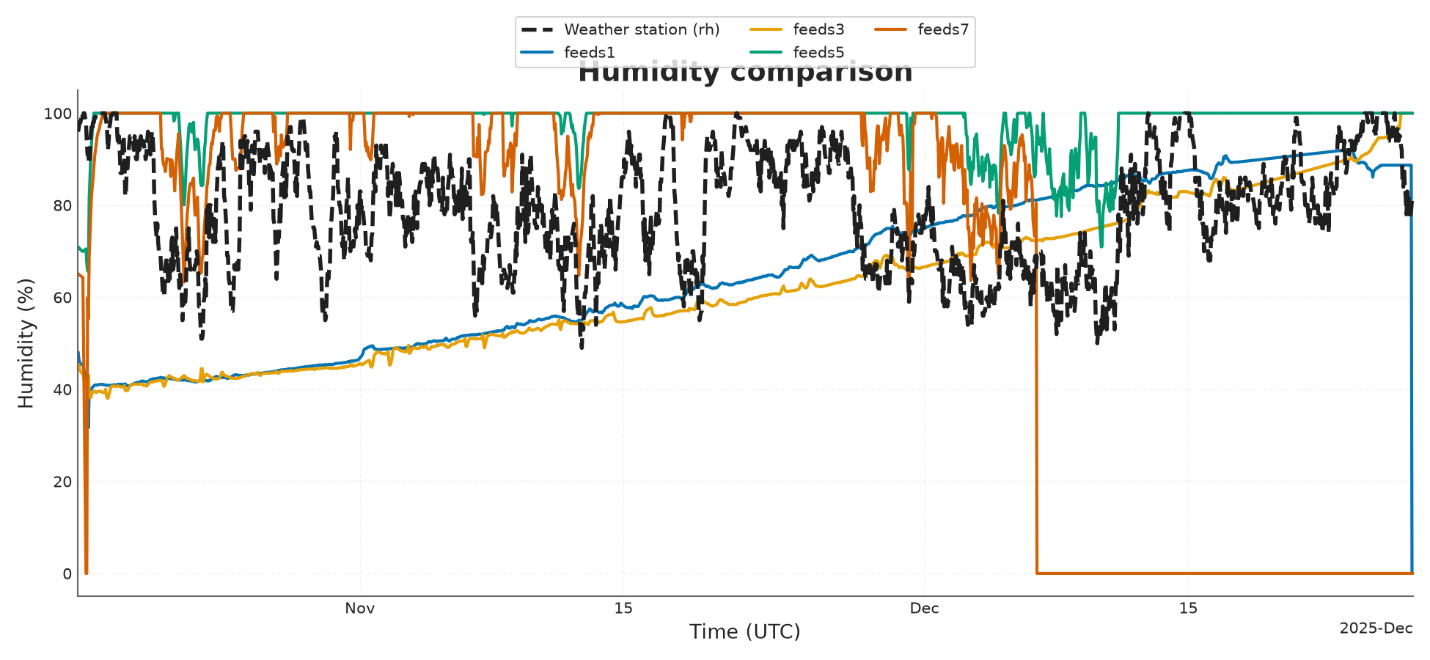
\includegraphics[width=\textwidth,height=3in,keepaspectratio]{figs/results-image8.png}
\caption{\draftchange{Comparison of relative humidity measurements from the deployed sensor nodes and the Sámsstaðir station (samst, 6222).}}
\label{fig:results-13}
\end{figure}

\draftchange{The relative humidity measurements from Sensor Nodes 5 and 7, which used externally mounted atmospheric sensors, showed broad variations that were generally comparable with the observations from the Sámsstaðir weather station. However, the comparison should be treated as qualitative because the weather station is located approximately 9.75 km from the deployment site and does not measure the exact same local conditions.}

\draftchange{Some deployed sensors produced readings that were not suitable for interpreting actual humidity variations. In particular, Sensor Node 3 recorded relative humidity values close to 100\% for an extended period toward the end of its reporting record. These readings cannot be treated as reliable evidence of the actual surrounding humidity.}

\draftchange{The available data do not establish why these readings occurred. The cause may be related to sensor exposure, moisture, the sensor environment, or another hardware or measurement issue, but the devices were not retrieved for inspection. Therefore, no specific cause should be assigned.}

\draftchange{Although the externally mounted sensors generally showed a more responsive pattern, the deployment was not a controlled experiment of sensor placement. Differences between locations and environmental exposure may also have influenced the results. Further testing would be needed to establish the effect of enclosure placement on humidity measurements.}

\subsection{Soil Temperature
Performance}

\draftchange{Figure~\ref{fig:results-14} illustrates the soil temperature measurements collected by the four buried sensor nodes together with ground-level temperature data from the Sámsstaðir station (samst, 6222).}

\begin{figure}[htbp]
\centering
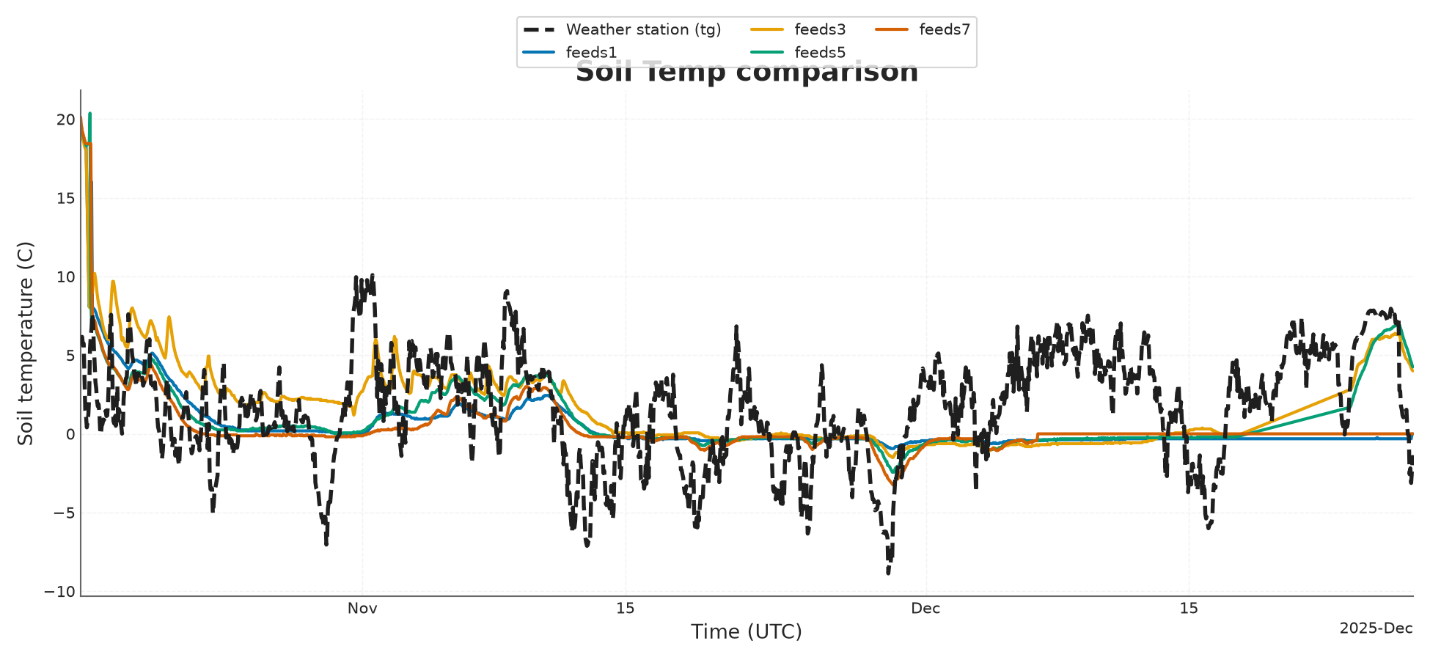
\includegraphics[width=\textwidth,height=3in,keepaspectratio]{figs/results-image9.png}
\caption{\draftchange{Comparison of soil temperature measurements from the deployed sensor nodes and ground-level data from the Sámsstaðir station (samst, 6222).}}
\label{fig:results-14}
\end{figure}

\draftchange{Unlike air temperature, soil temperature measurements from all four deployed nodes exhibited similar behavior regardless of installation configuration. The measured soil temperatures were significantly more stable than the air temperature recorded at station 6222, remaining close to the freezing point for much of the observation period. Rapid daily fluctuations in station 6222's air-temperature record were heavily damped by the thermal mass of the turf roof and surrounding soil.}

This behavior is expected since soil naturally buffers rapid temperature
changes. Even when air temperatures varied between approximately
\textbf{−8 °C and +10 °C}, soil temperatures remained close to \textbf{0
°C} with only gradual seasonal variation.

\draftchange{Station 6222 does \textbf{not} provide underground soil temperature measurements at the same depth as the deployed sensors. The comparison therefore used the station's \textbf{ground-level (surface) temperature} data as the closest available reference. Since the developed sensor nodes measured soil temperature at depths ranging from approximately \textbf{60 mm to 85 mm} below the turf surface (Figure~\ref{fig:results-deployment-map}), some difference between the two datasets was expected. Soil temperatures below the surface are naturally more thermally stable and less affected by rapid atmospheric temperature changes than temperatures measured at or near the ground surface.}

\draftchange{Consequently, the average absolute difference between the deployed sensor measurements and station 6222 data ranged from approximately \textbf{2.77 °C to 3.11 °C}. This is not a direct accuracy measurement, because the temperatures were measured at different locations and depths and under different environmental conditions. The Sámsstaðir comparison therefore does not independently validate the accuracy of the buried sensors.}

\draftchange{Overall, the measurements demonstrated stable soil-temperature trends during the deployment, consistent with the thermal buffering effect of the soil and turf. A reference sensor installed at the same location and depth as the deployed sensors would be required for a more direct comparison.}

\subsection{Individual Sensor
Performance}

\draftchange{The complete time-series measurements for Sensor Nodes 1, 3, 5, and 7 are presented in Figures~\ref{fig:results-15}, \ref{fig:results-16}, \ref{fig:results-8}, and \ref{fig:results-9}, respectively.}

\clearpage
\subparagraph{Sensor Node 1}

\draftchange{This node} maintained stable communication throughout most of the
deployment while continuously monitoring environmental conditions. Soil
moisture measurements remained relatively low with gradual increases
following wetter periods before decreasing as drainage occurred. Battery
voltage gradually decreased from approximately \textbf{4.1 V} to
\draftchange{\textbf{3.63 V}}, demonstrating efficient power consumption. \draftchange{The last valid ThingSpeak record from this node was received on 26 December 2025, an elapsed span of approximately 70.8 days from the first record. The final valid battery voltage was 3.63 V. The reason that subsequent valid measurements were no longer received is unknown.}

\begin{figure}[htbp]
\centering
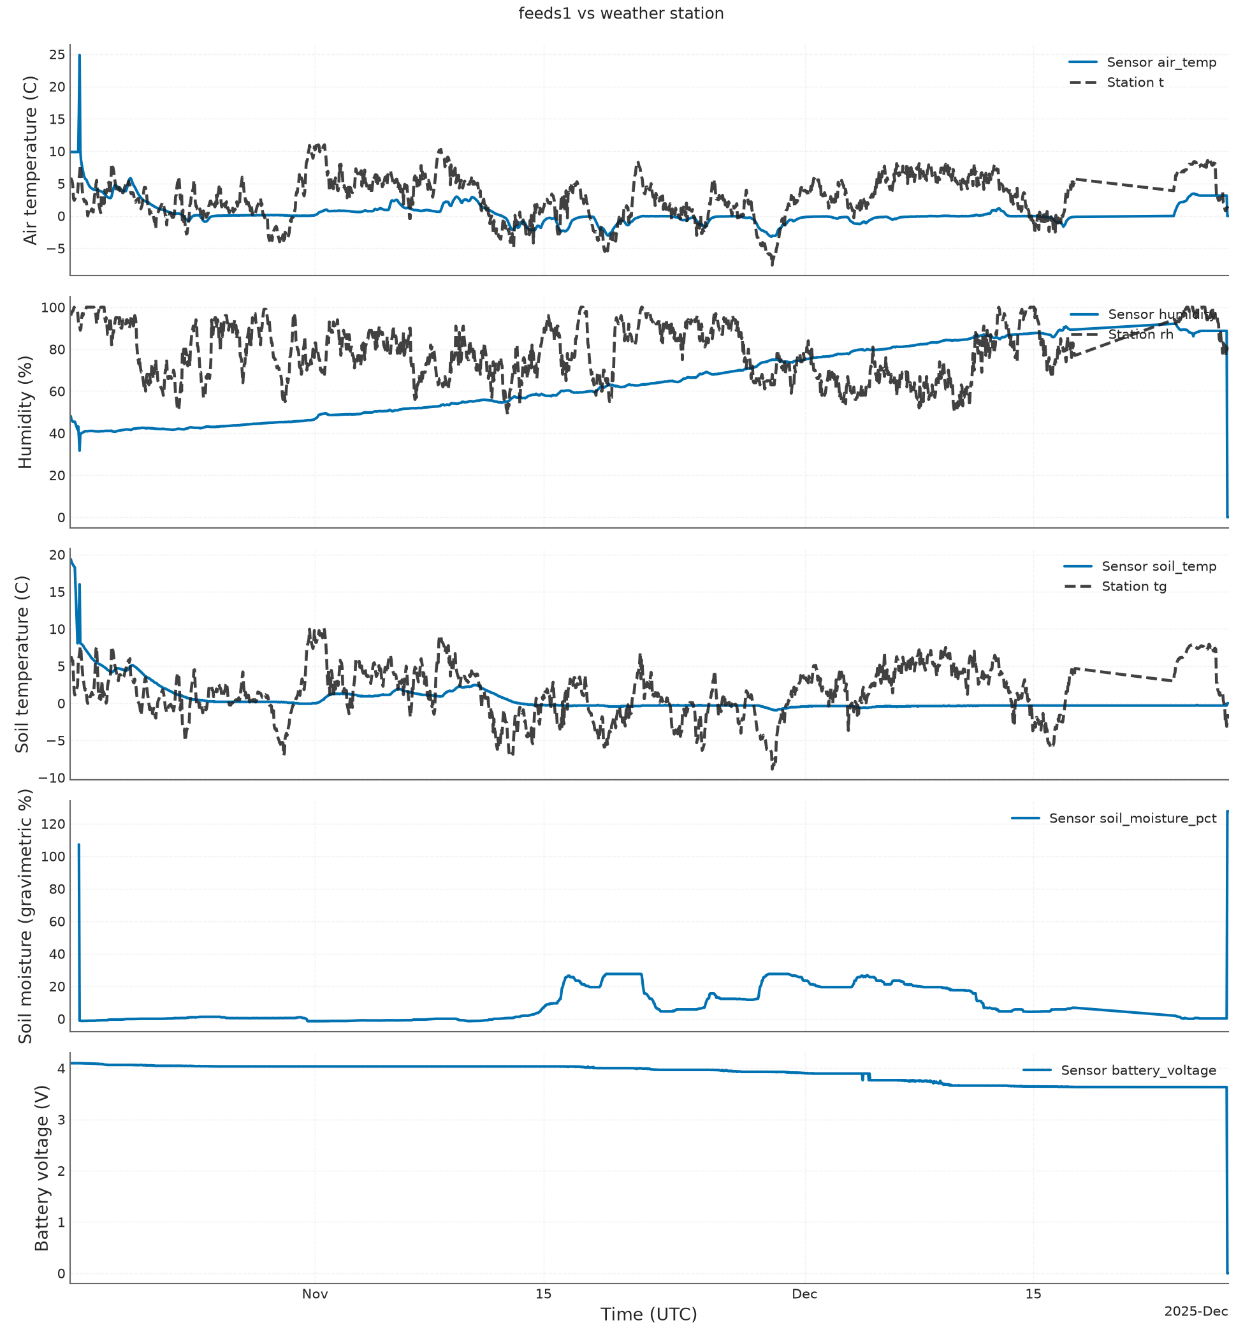
\includegraphics[width=5.63542in,height=6.06891in]{figs/results-image10.png}
\caption{Environmental measurements recorded by Sensor Node 1 throughout the deployment period.\draftchange{ Soil moisture is shown as raw ADC readings.}}
\label{fig:results-15}
\end{figure}

\clearpage
\subparagraph{Sensor Node 3}

\draftchange{Sensor Node 3 produced the longest valid ThingSpeak record, with a first-to-last valid reporting span of approximately 129.5 days, ending on 23 February 2026. The final valid entry reported a battery voltage of 3.49 V. This span includes the common interruption described in Section~\ref{sec:keldur-overall} and therefore does not represent uninterrupted uploads or a confirmed battery lifetime. The relative humidity readings from this node remained close to 100\% for an extended period near the end of its record and should be treated cautiously (Section~\ref{sec:keldur-humidity}).} \draftchange{Soil moisture increased during wetter conditions before gradually decreasing as the roof dried. Battery voltage showed a smooth and consistent discharge profile while the node was reporting.}

\begin{figure}[htbp]
\centering
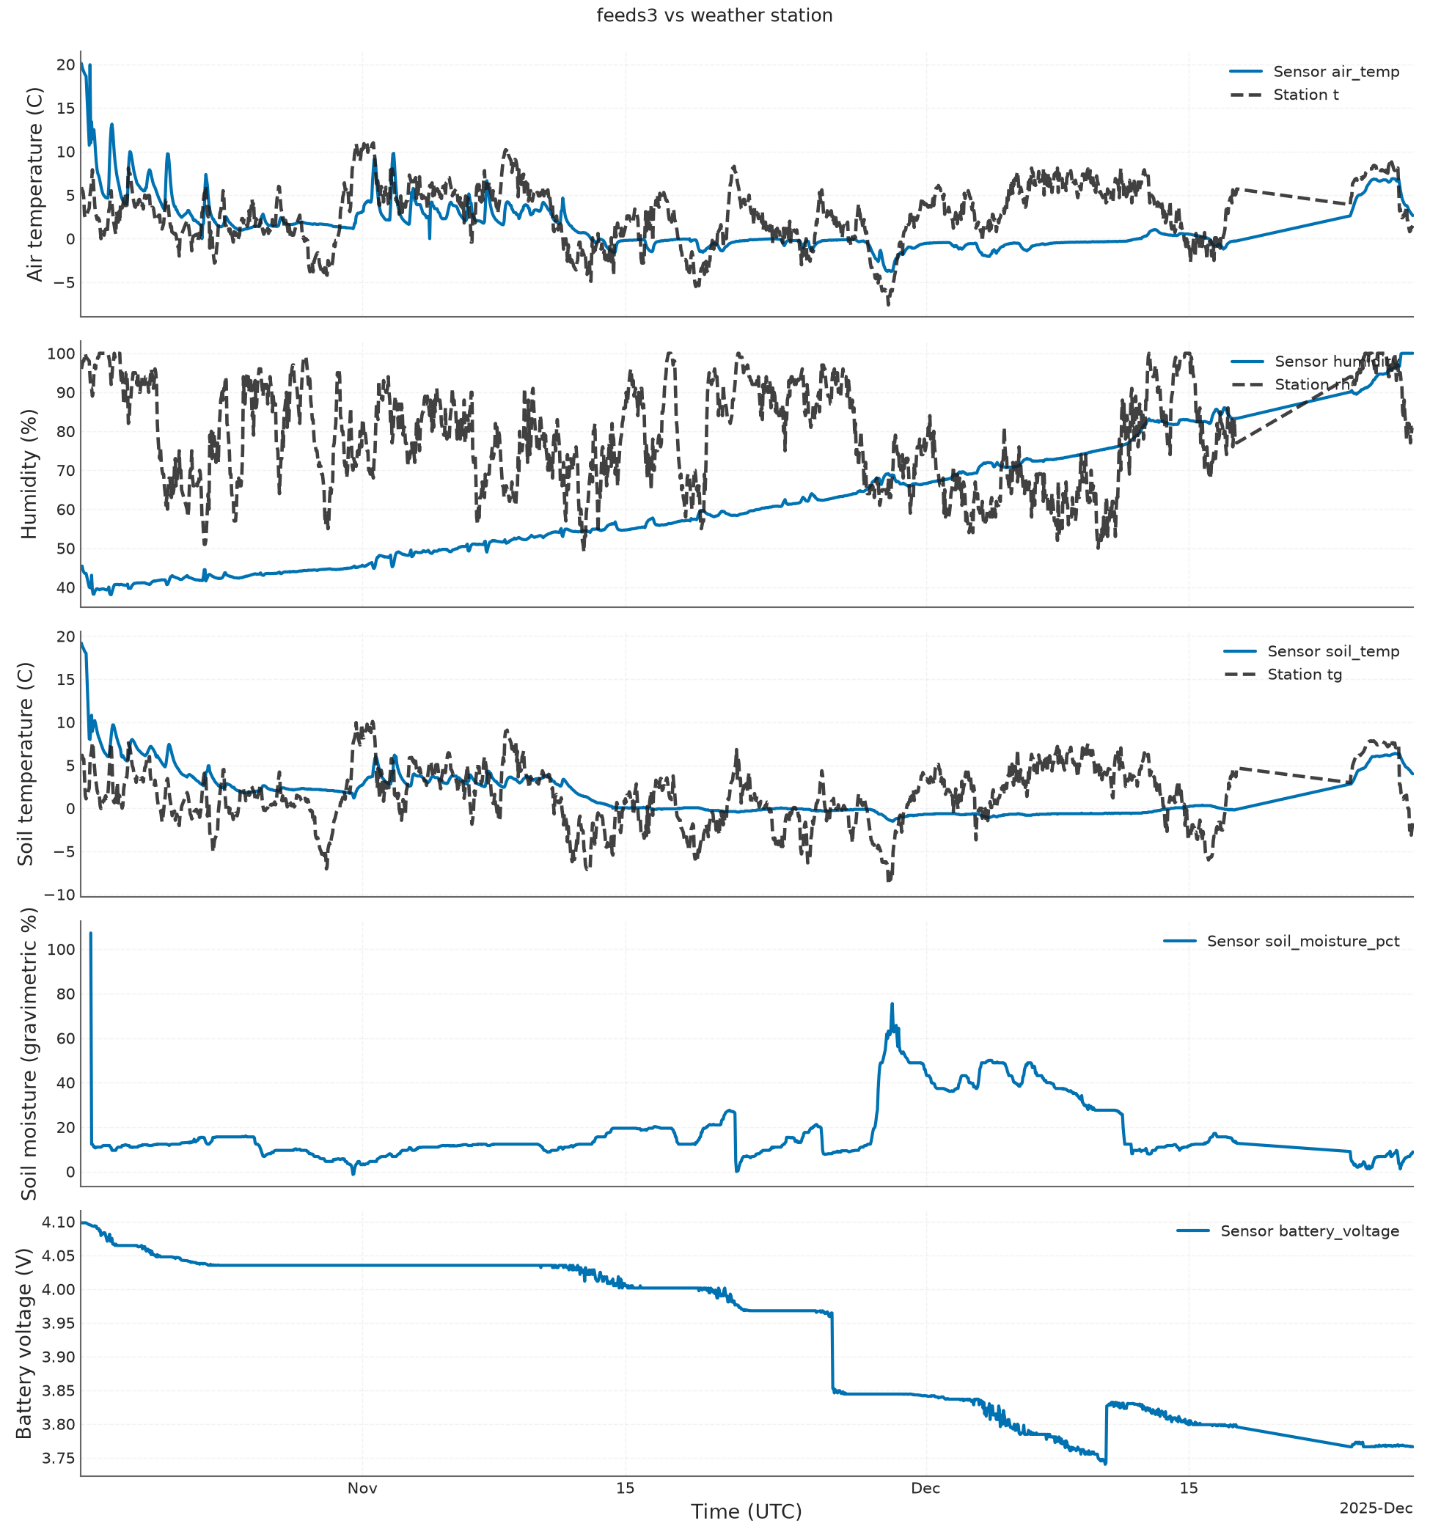
\includegraphics[width=\textwidth,height=7in,keepaspectratio]{figs/results-image11.png}
\caption{Environmental measurements recorded by Sensor Node 3 throughout the deployment period.\draftchange{ Soil moisture is shown as raw ADC readings.}}
\label{fig:results-16}
\end{figure}

\clearpage
\subparagraph{Sensor Node 5}

\draftchange{This node produced air temperature measurements that closely matched station 6222, consistent with its externally mounted atmospheric sensors. Its relative humidity readings are discussed in Section~\ref{sec:keldur-humidity}. Soil moisture remained consistently higher than the other deployed nodes, suggesting that its installation location retained more water within the turf roof. The reported battery voltage decreased gradually during the period for which valid measurements were received. The last valid ThingSpeak record was received on 2 January 2026, an elapsed span of approximately 77.5 days from the first record, with a final valid battery voltage of 3.78 V.}

\begin{figure}[htbp]
\centering
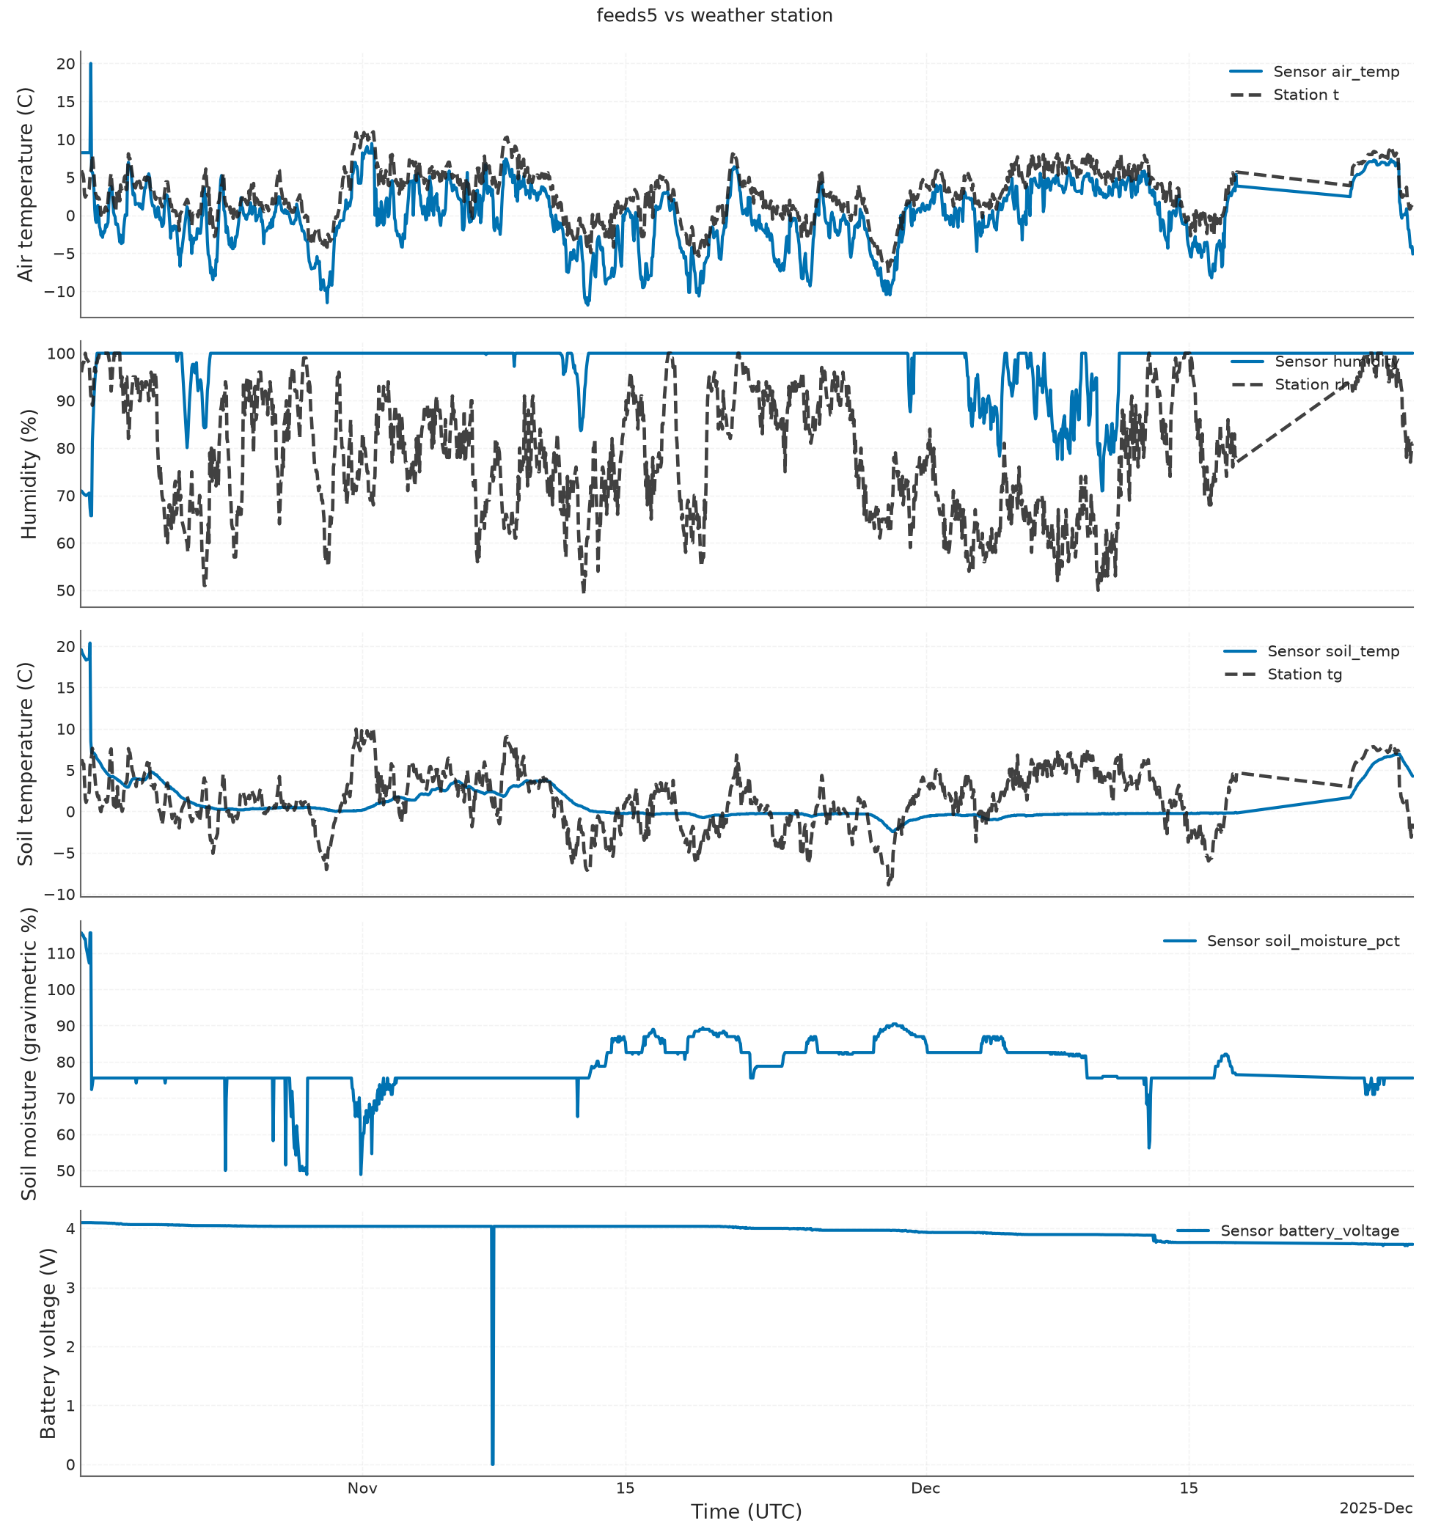
\includegraphics[width=\textwidth,height=7in,keepaspectratio]{figs/results-image12.png}
\caption{Environmental measurements recorded by Sensor Node 5 throughout the deployment period.\draftchange{ Soil moisture is shown as raw ADC readings.}}
\label{fig:results-8}
\end{figure}

\clearpage
\subparagraph{Sensor Node 7}

\draftchange{Sensor Node 7 provided valid measurements from 17 October 2025 through 6 December 2025, an elapsed span of approximately 50.9 days. The last valid ThingSpeak record reported a battery voltage of 3.93 V. The subsequent all-zero entries in the ThingSpeak feed are placeholders for missing measurements, not genuine zero-voltage or zero-humidity readings. The reason that this node stopped providing valid measurements is unknown.}

\begin{figure}[htbp]
\centering
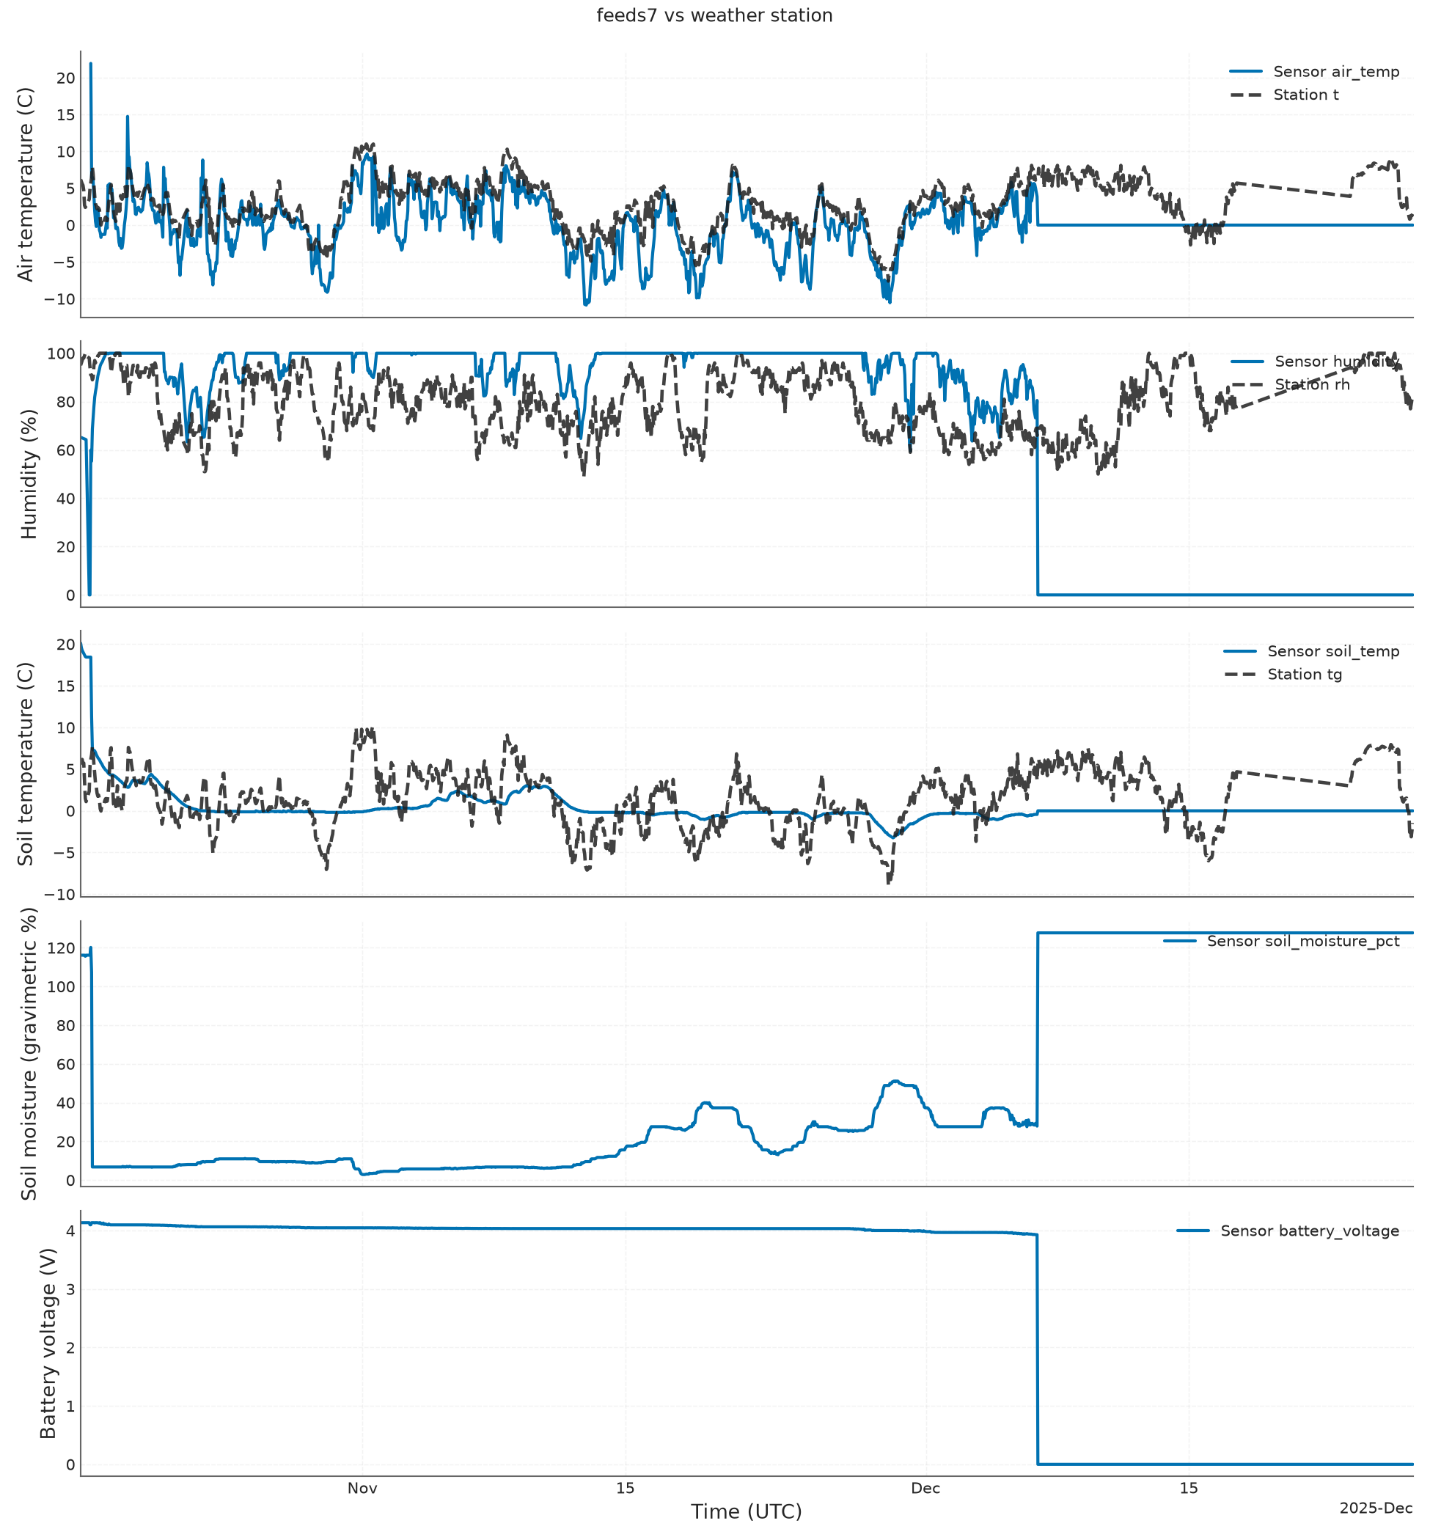
\includegraphics[width=\textwidth,height=7in,keepaspectratio]{figs/results-image13.png}
\caption{Environmental measurements recorded by Sensor Node 7 throughout the deployment period.\draftchange{ Soil moisture is shown as raw ADC readings.}}
\label{fig:results-9}
\end{figure}

\begin{table}[htbp]
\centering
\caption{\draftchange{Summary of valid ThingSpeak records and final reported battery voltages for the four Keldur sensor nodes.}}
\label{tab:keldur-record-span}
\begingroup
\color{purple}
\begin{tabular}{l l l c c}
\hline
Node & First record & Last record & Elapsed span & Final battery \\
\hline
1 & 17 Oct 2025 & 26 Dec 2025 & $\sim$70.8 days & 3.63 V \\
3 & 17 Oct 2025 & 23 Feb 2026 & $\sim$129.5 days & 3.49 V \\
5 & 17 Oct 2025 & 2 Jan 2026 & $\sim$77.5 days & 3.78 V \\
7 & 17 Oct 2025 & 6 Dec 2025 & $\sim$50.9 days & 3.93 V \\
\hline
\end{tabular}
\endgroup
\end{table}

\draftchange{The periods shown in Table~\ref{tab:keldur-record-span} represent the elapsed time between the first and last valid records received by ThingSpeak for each sensor node. They should not be interpreted as uninterrupted operating times or confirmed battery lifetimes, since missing records occurred during the deployment. The timestamps are based on the ThingSpeak \texttt{created\_at} field and therefore represent upload times rather than the sensor nodes' internal RTC measurement timestamps.}

\draftchange{The final valid battery voltages recorded for all four nodes remained above the configured 3.25 V cutoff. Since the sensor nodes were not retrieved at the end of the deployment, the reason each node stopped providing valid measurements could not be confirmed. Battery depletion should therefore not be presented as the cause.}

\draftchange{The ThingSpeak exports also contain all-zero entries after the last valid record of Sensor Nodes 1, 5, and 7. The base-station firmware clears its measurement arrays to zero at the start of each collection cycle, so when no valid new measurement is received from a node, these values can be uploaded as placeholders. These entries represent missing measurements rather than actual zero sensor readings. The soil-moisture values shown in the node plots are raw ADC readings from the capacitive sensors and are not converted to moisture percentages.}

\subsection{Overall System
Performance}\label{sec:keldur-overall}

\draftchange{The Keldur deployment demonstrated that the developed sensor nodes and base station could be installed beneath four separate turf roofs and used to collect environmental measurements under real outdoor conditions. The system recorded soil moisture, soil temperature, air temperature, relative humidity, and battery voltage, with measurements from the deployed nodes being delivered to ThingSpeak over different reporting periods.}

\draftchange{The reporting periods varied between nodes. Based on the first and last valid ThingSpeak records (Table~\ref{tab:keldur-record-span}), the elapsed spans ranged from approximately 50.9 days for Sensor Node 7 to 129.5 days for Sensor Node 3. These periods included missing records and should not be interpreted as uninterrupted operation or confirmed battery life. The last valid battery voltages were between 3.49 V and 3.93 V, all above the configured 3.25 V cutoff. Since the nodes were not retrieved, the reasons for the individual reporting endpoints remain unknown.}

\draftchange{A common interruption of approximately 145 hours was observed in the valid records from Sensor Nodes 1, 3, and 5, between 17 December and 23 December 2025. The available data do not identify the cause. Since these nodes experienced a similar interruption, it may have affected a shared part of the data collection or upload path. However, there are no retained base-station logs that would allow the interruption to be attributed to the LoRa communication, base station, internet connection, or another specific cause. Sensor Node 7 had already stopped providing valid measurements earlier, on 6 December 2025.}

\draftchange{The mesh communication algorithm was enabled on all four deployed sensor nodes. The firmware allowed nodes to receive, merge, and rebroadcast collected ledger data. However, no base-station packet logs were retained during the Keldur deployment. Consequently, it is not possible to determine whether particular measurements reached the base station directly or were forwarded through another sensor node. The deployment demonstrates that the implemented system collected and delivered data from four nodes, but it does not provide quantitative evidence of the individual multi-hop routes used.}

\draftchange{The separate range test conducted at Vellir demonstrated single-hop communication over an approximate 3 km radius. Mesh networking was not enabled during that range test, so its results should not be presented as a measured multi-hop range. An informal multi-hop test was also performed during firmware development (Section~\ref{sec:informal-multihop}), in which spaced sensor nodes relayed data until it reached the base station. This test was observed through debugging output, but no detailed logs, distances, packet counts, or route records were retained. It therefore provides qualitative evidence of the relay functionality rather than a reproducible performance measurement.}

\draftchange{Local SD-card backup was tested successfully during earlier field testing (Section~\ref{sec:sd-backup-testing}), where locally stored measurements were used to fill gaps in the base-station dataset. However, the Keldur node SD cards have not been retrieved, so this backup test cannot be used to claim that the missing Keldur records were recovered.}

\draftchange{Overall, the Keldur deployment demonstrated the practical feasibility of installing and operating the developed monitoring system at a real turf-roof site. It also identified important limitations involving missing measurements, uncertain node reporting endpoints, sensor data quality, and the lack of packet-level logging. Further field testing with retained communication logs and retrieved local data would be required to quantify long-term reliability and multi-hop performance.}

\section{Soil Moisture Calibration
Results}

\draftchange{The calibration results compare three measurement methods:
the gravimetric reference method, the HOBO MX2307 data logger,
and the custom capacitive soil moisture sensor.}

\subsection{Gravimetric Reference
Data}

Soil moisture calibration was performed using controlled samples at 0\%,
10\%, 20\%, 30\%, and 40\% moisture content. The gravimetric method was
used as the reference by adding known volumes of water to a measured
mass of dry soil.

Calibration was limited to 40\% moisture, as the soil approached
saturation beyond this point. Additional water produced minimal
dielectric variation, reducing the sensitivity of capacitive
measurements. \draftchange{The laboratory setup is shown in Figure~\ref{fig:calibration-setup}.}

\begin{figure}[htbp]
\centering
\subfigure[Calibration setup with the soil sample, custom sensors, and reference instrument.]{%
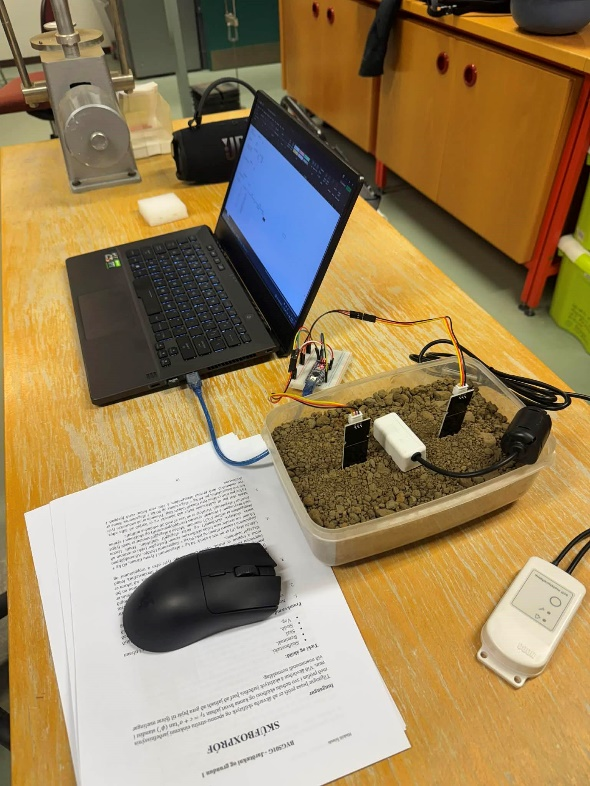
\includegraphics[width=2.67708in,height=3.56944in]{figs/results-image14.jpeg}}
\hfill
\subfigure[Custom sensors installed in the prepared soil sample.]{%
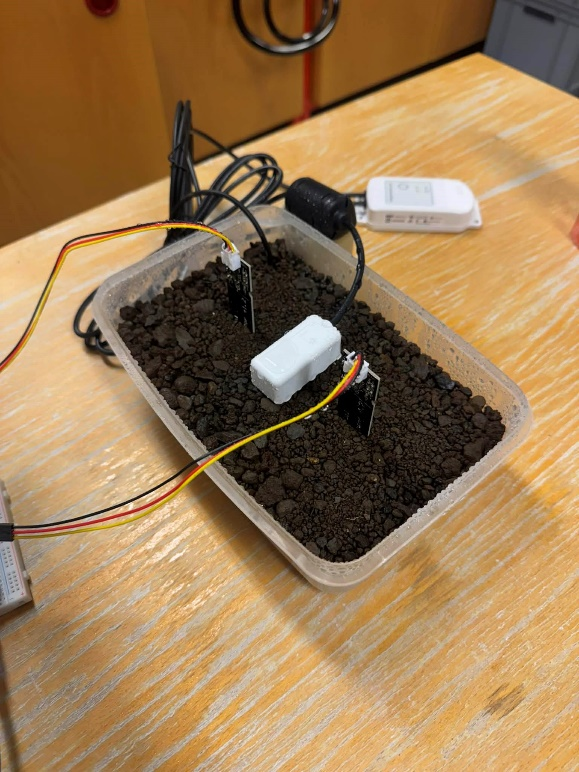
\includegraphics[width=2.67708in,height=3.56944in]{figs/results-image15.jpeg}}
\caption{Laboratory setup used for the soil moisture sensor calibration tests.}
\label{fig:calibration-setup}
\end{figure}

\clearpage
Two calibration tests were conducted.

\textbf{Test 1 (2069.5 g soil sample):}

\begin{longtable}[]{@{}
  >{\raggedright\arraybackslash}p{(\columnwidth - 8\tabcolsep) * \real{0.2254}}
  >{\raggedright\arraybackslash}p{(\columnwidth - 8\tabcolsep) * \real{0.2361}}
  >{\raggedright\arraybackslash}p{(\columnwidth - 8\tabcolsep) * \real{0.1758}}
  >{\raggedright\arraybackslash}p{(\columnwidth - 8\tabcolsep) * \real{0.1804}}
  >{\raggedright\arraybackslash}p{(\columnwidth - 8\tabcolsep) * \real{0.1822}}@{}}
\caption{Calibration Test 1 results for the 2069.5 g soil sample.}
\label{tab:calibration-test-1}\\
\toprule\noalign{}
\begin{minipage}[b]{\linewidth}\raggedright
\textbf{Soil Moisture (\%)}
\end{minipage} & \begin{minipage}[b]{\linewidth}\raggedright
\textbf{Water Added (mL)}
\end{minipage} & \begin{minipage}[b]{\linewidth}\raggedright
\textbf{VWC (m³/m³)}
\end{minipage} & \begin{minipage}[b]{\linewidth}\raggedright
\textbf{Raw Sensor 1}
\end{minipage} & \begin{minipage}[b]{\linewidth}\raggedright
\textbf{Raw Sensor 2}
\end{minipage} \\
\midrule\noalign{}
\endfirsthead
\endhead
\bottomrule\noalign{}
\endlastfoot
0 & 0 & 0 & 483.52 & 486.26 \\
10 & 206.95 & 0.15 & 314.17 & 324.55 \\
20 & 413.9 & 0.27 & 232.17 & 239.29 \\
30 & 620.85 & 0.33 & 223.26 & 216.67 \\
40 & 827.8 & 0.39 & 193.20 & 201.16 \\
\end{longtable}

The large sample size resulted in long saturation times and difficult
handling.

\textbf{Test 2 (400 g soil sample):}

\begin{longtable}[]{@{}
  >{\raggedright\arraybackslash}p{(\columnwidth - 6\tabcolsep) * \real{0.2750}}
  >{\raggedright\arraybackslash}p{(\columnwidth - 6\tabcolsep) * \real{0.2881}}
  >{\raggedright\arraybackslash}p{(\columnwidth - 6\tabcolsep) * \real{0.2145}}
  >{\raggedright\arraybackslash}p{(\columnwidth - 6\tabcolsep) * \real{0.2224}}@{}}
\caption{Calibration Test 2 results for the 400 g soil sample.}
\label{tab:calibration-test-2}\\
\toprule\noalign{}
\begin{minipage}[b]{\linewidth}\raggedright
\textbf{Soil Moisture (\%)}
\end{minipage} & \begin{minipage}[b]{\linewidth}\raggedright
\textbf{Water Added (mL)}
\end{minipage} & \begin{minipage}[b]{\linewidth}\raggedright
\textbf{VWC (m³/m³)}
\end{minipage} & \begin{minipage}[b]{\linewidth}\raggedright
\textbf{Raw Sensor 1}
\end{minipage} \\
\midrule\noalign{}
\endfirsthead
\endhead
\bottomrule\noalign{}
\endlastfoot
0 & 0 & 0.02 & 482.55 \\
10 & 40 & 0.21 & 260.36 \\
20 & 80 & 0.29 & 265.29 \\
30 & 120 & 0.34 & 220.68 \\
40 & 160 & 0.39 & 202.52 \\
\end{longtable}

The second test improved practicality while maintaining consistent
trends. In both tests, ADC values decreased as moisture increased,
confirming expected capacitive sensor behavior.

\subsection{HOBO Sensor and Dielectric
Reference}

A HOBO MX2307 (TEROS-10 probe) was used as a reference. It measures
dielectric permittivity and converts it to volumetric water content
(VWC) using:

\begin{equation}
\theta = 4.3 \times 10^{- 6}\varepsilon^{3} - 5.5 \times 10^{- 4}\varepsilon^{2} + 2.92 \times 10^{- 2}\varepsilon - 5.3 \times 10^{- 2}
\label{eq:dielectric-moisture-calibration}
\end{equation}

Measured VWC values were back-calculated to obtain dielectric
permittivity:

\begin{longtable}[]{@{}
  >{\raggedright\arraybackslash}p{(\columnwidth - 4\tabcolsep) * \real{0.2233}}
  >{\raggedright\arraybackslash}p{(\columnwidth - 4\tabcolsep) * \real{0.3442}}
  >{\raggedright\arraybackslash}p{(\columnwidth - 4\tabcolsep) * \real{0.4325}}@{}}
\caption{HOBO reference measurements and calculated dielectric permittivity.}
\label{tab:hobo-dielectric-reference}\\
\toprule\noalign{}
\begin{minipage}[b]{\linewidth}\raggedright
\textbf{Moisture (\%)}
\end{minipage} & \begin{minipage}[b]{\linewidth}\raggedright
\textbf{HOBO VWC (m³/m³)}
\end{minipage} & \begin{minipage}[b]{\linewidth}\raggedright
\textbf{Dielectric Permittivity (ε)}
\end{minipage} \\
\midrule\noalign{}
\endfirsthead
\endhead
\bottomrule\noalign{}
\endlastfoot
0 & 0.01 & 2.251 \\
10 & 0.18 & 9.578 \\
20 & 0.28 & 15.273 \\
30 & 0.335 & 19.175 \\
40 & 0.39 & 23.957 \\
\end{longtable}

Dielectric permittivity increased with moisture due to the high
dielectric constant of water.

\subsection{Polynomial Calibration
Model}

Due to the nonlinear relationship between ADC output and soil moisture,
a second-order polynomial regression was applied:

\begin{equation}
\text{Soil~Moisture~(\%)} = 0.0006877(\text{ADC})^{2} - 0.5961(\text{ADC}) + 127.70
\label{eq:adc-soil-moisture-calibration}
\end{equation}

\draftchange{The second-order polynomial was fitted using the arithmetic mean of the two capacitive sensor readings from Test 1 at each gravimetric moisture level. The resulting coefficients are presented in Equation~\ref{eq:adc-soil-moisture-calibration}. Table~\ref{tab:averaged-calibration-data} separately summarizes the average of all three capacitive sensor readings collected across both calibration tests. The two datasets should not be confused: the polynomial coefficients correspond to the Test 1 averages shown in Table~\ref{tab:final-calibration-results}, rather than the combined averages in Table~\ref{tab:averaged-calibration-data}.}

\begin{longtable}[]{@{}
  >{\raggedright\arraybackslash}p{(\columnwidth - 4\tabcolsep) * \real{0.3592}}
  >{\raggedright\arraybackslash}p{(\columnwidth - 4\tabcolsep) * \real{0.2606}}
  >{\raggedright\arraybackslash}p{(\columnwidth - 4\tabcolsep) * \real{0.3802}}@{}}
\caption{\draftchange{Overall average calibration data from both tests (all three capacitive sensor readings); these are not the input data used for the polynomial in Equation~\ref{eq:adc-soil-moisture-calibration}.}}
\label{tab:averaged-calibration-data}\\
\toprule\noalign{}
\begin{minipage}[b]{\linewidth}\raggedright
\textbf{Moisture (\%)}
\end{minipage} & \begin{minipage}[b]{\linewidth}\raggedright
\textbf{Avg VWC}
\end{minipage} & \begin{minipage}[b]{\linewidth}\raggedright
\textbf{Raw Avg ADC}
\end{minipage} \\
\midrule\noalign{}
\endfirsthead
\endhead
\bottomrule\noalign{}
\endlastfoot
0 & 0.01 & 484.11 \\
10 & 0.18 & 299.69 \\
20 & 0.28 & 245.58 \\
30 & 0.335 & 220.20 \\
40 & 0.39 & 198.96 \\
\end{longtable}

\clearpage
\subsection{Final Calibration Results and
Discussion}

\begin{longtable}[]{@{}
  >{\raggedright\arraybackslash}p{(\columnwidth - 8\tabcolsep) * \real{0.2534}}
  >{\raggedright\arraybackslash}p{(\columnwidth - 8\tabcolsep) * \real{0.1114}}
  >{\raggedright\arraybackslash}p{(\columnwidth - 8\tabcolsep) * \real{0.1921}}
  >{\raggedright\arraybackslash}p{(\columnwidth - 8\tabcolsep) * \real{0.2096}}
  >{\raggedright\arraybackslash}p{(\columnwidth - 8\tabcolsep) * \real{0.2336}}@{}}
\caption{\draftchange{Comparison of gravimetric moisture, Test 1 mean ADC, HOBO, dielectric, and polynomial output values.}}
\label{tab:final-calibration-results}\\
\toprule\noalign{}
\begin{minipage}[b]{\linewidth}\raggedright
\textbf{Gravimetric (\%)}
\end{minipage} & \begin{minipage}[b]{\linewidth}\raggedright
\textbf{\draftchange{Test 1 Mean ADC}}
\end{minipage} & \begin{minipage}[b]{\linewidth}\raggedright
\textbf{HOBO VWC}
\end{minipage} & \begin{minipage}[b]{\linewidth}\raggedright
\textbf{Dielectric (ε)}
\end{minipage} & \begin{minipage}[b]{\linewidth}\raggedright
\textbf{\draftchange{Polynomial Output (\%)}}
\end{minipage} \\
\midrule\noalign{}
\endfirsthead
\endhead
\bottomrule\noalign{}
\endlastfoot
0 & 484.89 & 0.01 & 2.251 & \draftchange{0.35} \\
10 & 319.36 & 0.18 & 9.578 & \draftchange{7.47} \\
20 & 235.73 & 0.28 & 15.273 & \draftchange{25.40} \\
30 & \draftchange{219.97} & 0.335 & 19.175 & \draftchange{29.85} \\
40 & 197.18 & 0.39 & 23.957 & \draftchange{36.90} \\
\end{longtable}

\draftchange{The polynomial model produced an RMSE of approximately 3.01 percentage points when its calculated moisture values were compared with the gravimetric moisture targets at the five calibration levels. This value represents the fit error on the same calibration data used to derive the polynomial. It is therefore an in-sample calibration error rather than an independent validation result.}

\draftchange{For comparison, converting the HOBO VWC values to percentages and comparing them with the polynomial outputs gives an RMSE of approximately 5.21 percentage points over the same five calibration levels. This comparison provides an indication of the difference between the two measurement methods, but it should not be described as independent validation because the readings were collected during the same calibration procedure.}

\draftchange{The calibration was conducted using a separate Icelandic soil sample rather than soil collected from the Keldur deployment locations. Although the same capacitive sensor model and supply voltage were used, the soil composition and characteristics may differ. As a result, the calibration relationship cannot automatically be assumed to apply to all Keldur soil conditions.}

\draftchange{The Keldur ThingSpeak data further show that a substantial portion of the raw ADC readings falls outside the ADC range used to fit the polynomial, approximately 197.18--484.89. Using records with a non-zero battery-voltage field and excluding the all-zero placeholder entries, the median raw ADC values were approximately 527 for Node 1, 575 for Node 3, 768 for Node 5, and 568 for Node 7. Only approximately 31.1\% of Node 1 readings and 0.8\% of Node 3 readings fell within the calibration range. No readings from Nodes 5 and 7 fell within that range.}

\draftchange{These results mean that applying the polynomial to the full Keldur datasets would require extrapolation for most measurements. Such extrapolation would not be reliable. Therefore, the Keldur soil-moisture plots should remain in raw ADC units rather than being converted into volumetric water content or calibrated moisture percentages using this polynomial.}

\draftchange{The calibration demonstrates that the capacitive sensor has a nonlinear response to controlled changes in soil moisture over the tested 0--40\% range. However, further calibration using soil collected from the actual turf-roof locations, together with independent reference measurements, is required before quantitative soil-moisture values can be confidently reported for the Keldur deployment.}

\section{Cloud Upload Performance
(ThingSpeak)}

\draftchange{The cloud upload functionality was evaluated using the ThingSpeak IoT
platform. Sensor data from the base station---including soil moisture,
temperature, humidity, battery voltage, and timestamps---was transmitted
via Wi-Fi using HTTP GET requests. During testing, the uploaded sensor
data was successfully received by the ThingSpeak server, with the
requests consistently returning an HTTP response code of \emph{200 OK}.
The average upload time was approximately 1--2 seconds, depending on
network conditions.}

\draftchange{The integration made the collected sensor measurements available through ThingSpeak for remote access, visualization, and further analysis. The observed upload time was suitable for the periodic data-transfer requirements of the monitoring system.}

\draftchange{These results describe the controlled cloud-upload tests. They confirm that the upload process worked during the recorded tests, but they do not establish uninterrupted cloud availability or upload success throughout the Keldur field deployment.}


\chapter{Conclusion and Recommendations}

\draftchange{This project demonstrated that a low-cost, low-power LoRa-based wireless sensor network can be built and deployed to monitor environmental conditions beneath Icelandic turf roofs. Four sensor nodes were built and deployed beneath four separate turf roofs at Keldur. The system combines custom sensor nodes, local data storage, LoRa communication, a base station, and ThingSpeak cloud integration.}

\draftchange{Power consumption tests showed an average current of approximately 3.08 mA. Based on the nominal capacity of 10,500 mAh (three 3,500 mAh cells in parallel), the theoretical battery lifetime was estimated at approximately 142 days under the documented operating cycle. This is an estimate and not a measured field lifetime, and low temperatures can reduce the actual battery capacity.}

\draftchange{Field range testing around Vellir in Hafnarfjörður demonstrated approximately 3 km of single-hop communication using suitable 433 MHz antennas. Mesh networking was not enabled during this test. The tests also showed how antenna selection and placement affect communication performance.}

\draftchange{The deployment at Keldur demonstrated the system's ability to monitor four separate turf roofs under real outdoor conditions. Measurements from the four sensor nodes were collected and delivered to ThingSpeak over different periods. The first-to-last valid record spans were approximately 70.8 days for Node 1, 129.5 days for Node 3, 77.5 days for Node 5, and 50.9 days for Node 7. These are first-to-last valid record spans, not uninterrupted uptime or confirmed battery life.}

\draftchange{The last valid battery voltages were 3.63 V, 3.49 V, 3.78 V, and 3.93 V for Nodes 1, 3, 5, and 7, respectively, all above the configured 3.25 V cutoff. The available data do not establish that battery depletion caused the nodes to stop providing valid measurements, and the reasons for the individual reporting endpoints are unknown. The nodes remain installed at Keldur and have not been retrieved for physical inspection.}

\draftchange{A common data interruption of approximately 145 hours, between 17 and 23 December 2025, was observed in the valid records from Nodes 1, 3, and 5, but its cause could not be identified. The lack of persistent base-station logs limited the ability to distinguish between wireless communication interruptions and interruptions in the base-station or internet connection.}

\draftchange{The mesh firmware was implemented, and relay functionality was enabled on all four Keldur sensor nodes. In addition, an informal development-stage test provided qualitative evidence that the relay mechanism could forward ledger data between nodes and eventually deliver it to the base station. However, no retained packet logs prove the routes taken by individual measurements, so the actual use and performance of multi-hop paths during the Keldur deployment could not be quantified.}

\draftchange{Soil moisture calibration produced a second-order polynomial model with an in-sample RMSE of approximately 3.01 percentage points against the gravimetric calibration targets over the tested 0--40\% range. The comparison with HOBO values gives approximately 5.21 percentage points. Neither value represents independent field validation. Most Keldur raw soil-moisture readings were outside the calibration ADC range, so the field readings should not be presented as validated moisture percentages.}

\draftchange{ThingSpeak uploads took approximately 1--2 seconds during the upload tests and returned HTTP 200 OK responses, enabling remote access and visualization of the collected measurements.}

\draftchange{The six research objectives are assessed in Table~\ref{tab:objective-assessment}. Objectives 1, 3, and 6 were achieved. Objectives 2 and 5 were achieved with limitations, and Objective 4 was achieved in earlier field testing. The limitations are stated in the table and mainly concern the lack of quantitative multi-hop results and the lack of independent validation of the soil moisture calibration.}

\begin{table}[htbp]
\centering
\caption{\draftchange{Assessment of the research objectives.}}
\label{tab:objective-assessment}
\begingroup
\small
\color{purple}
\begin{tabularx}{\textwidth}{@{}>{\raggedright\arraybackslash}p{0.25\textwidth}>{\raggedright\arraybackslash}p{0.17\textwidth}>{\raggedright\arraybackslash}X@{}}
\toprule
\textbf{Objective} & \textbf{Assessment} & \textbf{Basis} \\
\midrule
1. Implement distributed sensor nodes & Achieved & Four sensor nodes were built and deployed to measure soil moisture, soil temperature, air temperature, relative humidity, and battery voltage. \\
2. Implement LoRa communication and evaluate range and field operation & Achieved with limitations & The communication system was implemented and used during the Keldur deployment. The Vellir test demonstrated approximately 3 km single-hop communication. Mesh relay functionality was implemented, but quantitative multi-hop performance and individual Keldur packet routes were not recorded. \\
3. Measure current consumption and estimate battery life & Achieved & The average current was measured at approximately 3.08 mA, and the approximately 142-day battery lifetime was estimated using the nominal battery capacity and measured operating cycle. The estimate does not represent a measured field lifetime. \\
4. Implement and evaluate local data storage & Achieved in earlier field testing & The SD-card backup was tested, and locally stored measurements were used to fill missing entries in the base-station dataset. Keldur SD-card data have not been retrieved or used. \\
5. Develop and evaluate the soil moisture calibration model & Achieved with limitations & A second-order polynomial model was developed over the tested 0--40\% gravimetric moisture range. The in-sample RMSE was approximately 3.01 percentage points. Independent validation and transfer to Keldur soil conditions were not established. \\
6. Integrate the network with a cloud platform & Achieved & The base station uploaded measurements to ThingSpeak during the cloud integration tests, with HTTP 200 OK responses and an average upload time of approximately 1--2 seconds. \\
\bottomrule
\end{tabularx}
\endgroup
\end{table}

\draftchange{Overall, the project demonstrated the feasibility of building and deploying an affordable remote monitoring system for Icelandic turf roofs. However, the results also show that further work is needed to improve long-term reliability, validate soil-moisture measurements in actual turf-roof soil, and quantitatively evaluate mesh routing.}

\section{Recommendations}
Future work should focus on extending the duration of field deployments, improving the reliability of individual sensor nodes, and expanding calibration and validation. In particular, the following improvements are recommended:
\begin{enumerate}
\item \draftchange{\textbf{Improve battery and power management:} conduct longer winter tests to evaluate actual battery performance at low temperatures and compare measured field operation with the theoretical estimate;}
\item \draftchange{\textbf{Improve enclosure and sensor protection:} improve protection against moisture, freezing, thawing, and snow, and continue evaluating external placement of atmospheric sensors while ensuring suitable weather protection. Future designs should allow sufficient airflow for ambient measurements while providing protection against direct rain and water accumulation, and both internal and externally mounted arrangements should be evaluated under controlled conditions;}
\item \draftchange{\textbf{Add remote system-health monitoring:} report node status, battery voltage, last successful measurement, and communication status so that missing measurements can be detected and investigated;}
\item \draftchange{\textbf{Improve local data logging:} retrieve and examine the Keldur node SD-card data where possible. Add local base-station logging, preferably using an SD card or equivalent storage, to retain packet IDs, node IDs, timestamps, RSSI/SNR, packet reception, forwarding events, and cloud-upload status. This would help distinguish missing LoRa transmissions from cloud-upload interruptions;}
\item \draftchange{\textbf{Improve soil-moisture calibration:} use soil collected from the actual turf-roof locations, test several samples, extend the moisture range where physically meaningful, and compare the results against co-located reference instruments. Use a separate dataset for validation;}
\item \draftchange{\textbf{Conduct controlled multi-hop testing:} deliberately place one or more sensor nodes outside the direct communication range of the base station and use intermediate nodes to relay their data. Measure packet delivery, RSSI/SNR, forwarding routes, hop count, latency, and reliability with different node distances and network topologies. Retain logs so the results can be reproduced; and}
\item \draftchange{\textbf{Continue long-term deployments:} evaluate the system at additional turf-roof locations and across different seasons and soil conditions.}
\end{enumerate}

\printbibliography[heading=bibintoc,title={References}]

\appendix
\chapter{Additional Material}
\markboth{A. Additional Material}{A. Additional Material}

\section{\texorpdfstring{\draftchange{Bill of Materials}}{Bill of Materials}}

\draftchange{The bill of materials lists the main components and materials used to construct one in situ sensor node, which is buried beneath the turf roof. It is organized into PCB assembly components and the additional modules and materials used in the implementation. The base station is not included because it is not buried and uses a different controller, the LOLIN D1 mini. The list serves as a reference for the sensor-node hardware described in this thesis.}

\draftchange{The total cost of the priced components and materials listed in the bill of materials for one sensor node is ISK 11,921.44. Components listed as ``Not priced'' or ``Not populated'' are not included in the total. For D2, either a 1N4001 or 1N4004 diode can be used; both are suitable for the intended application and have the same cost. The choice between the two was based on component availability.}

\subsection{\texorpdfstring{\draftchange{PCB Assembly}}{PCB Assembly}}

\begingroup
\small
\color{purple}

\markboth{A. Additional Material}{A. Additional Material}

\begin{longtable}{@{}p{0.20\textwidth}p{0.54\textwidth}>{\raggedleft\arraybackslash}p{0.18\textwidth}@{}}
\textbf{Reference} & \textbf{Component or value} & \textbf{Cost (ISK)} \\
\toprule
PCB & PCB fabrication & 137.00 \\
C1 & \(0.1~\mu\text{F}\) capacitor & 14.99 \\
C2--C4 & Three \(10~\mu\text{F}\) polarized capacitors & 19.19 \\
D1 & 1N4148 diode & 50.00 \\
D2 & 1N4001 or 1N4004 diode & 13.00 \\
H1--H2 & Mounting holes; listed price is for standoffs & 4.41 \\
J1--J2 & Battery positive and negative connections & Not priced \\
JP1--JP4 & Normally open jumpers & Not priced \\
JP5--JP6 & Ra-02 pin headers & 43.44 \\
JP7 & Ra-01 alternate header footprint & Not populated \\
JP8, JP9, JP15, JP17 & Power-selection jumpers & Not priced \\
JP10 & DS3231 header & 18.71 \\
JP11 & AHT10 header & 22.51 \\
JP12 & DS18B20 header & 26.18 \\
JP13 & Soil-moisture sensor header & 26.18 \\
JP14 & SD card header & 18.71 \\
JP16 & Debug header & Not populated \\
Q1--Q2 & ZVP2106A P-channel MOSFETs & 242.17 \\
R1, R3 & Two \(4.7~\text{k}\Omega\) resistors & 12.21 \\
R2, R7 & Two \(47~\text{k}\Omega\) resistors & 12.06 \\
R4 & \(10~\text{k}\Omega\) resistor & 6.13 \\
R5 & \(33~\text{k}\Omega\) resistor & 6.07 \\
R6, R8 & Two \(100~\text{k}\Omega\) resistors & 12.26 \\
SW1 & Three-position hardware-ID DIP switch & 50.53 \\
SW2 & Power DIP switch & 46.81 \\
T1--T2 & Two 2N2222 NPN transistors & 30.57 \\
U\$1 & ABK Pro Mini Arduino clone & 541.11 \\
-- & Two Pro Mini female headers, 1\texttimes 12 & 52.37 \\
-- & Pro Mini female header, 1\texttimes 2 & 22.51 \\
-- & Pro Mini female header, 1\texttimes 3 & 19.71 \\
-- & Pro Mini female header, 1\texttimes 6 & 21.57 \\
\bottomrule
\end{longtable}
\endgroup

\subsection{\texorpdfstring{\draftchange{Modules and Materials}}{Modules and Materials}}
\markboth{\draftchange{A. Additional Material}}{\draftchange{A. Additional Material}}
\begingroup
\small
\color{purple}
\begin{longtable}{@{}p{0.20\textwidth}p{0.54\textwidth}>{\raggedleft\arraybackslash}p{0.18\textwidth}@{}}
\textbf{Reference} & \textbf{Component or material} & \textbf{Cost (ISK)} \\
\toprule
-- & AHT10 temperature and humidity sensor module & 108.39 \\
-- & Shielded four-wire cable for the AHT10 & 155.27 \\
-- & SMA-to-uFL female RF adapter cable & 163.05 \\
-- & 433 MHz antenna & 163.05 \\
-- & DS3231 real-time clock module & 206.48 \\
-- & Ra-02 LoRa module with SX1278 transceiver & 949.97 \\
-- & 1 GB microSD card & 1,690.00 \\
-- & SD card serial logger module & 662.46 \\
-- & Waterproof DS18B20 temperature probe & 281.98 \\
-- & Capacitive soil-moisture sensor, v1.2 & 254.40 \\
-- & Three 18650 lithium-ion cells & 3,901.00 \\
-- & Parallel 18650 battery holder & 280.72 \\
-- & Waterproof enclosure for antenna and AHT10 & 213.62 \\
-- & Waterproof enclosure for sensor-node electronics & 420.62 \\
-- & Mounting screws, glue, solder, and miscellaneous materials & 1,000.00 \\
\midrule
\multicolumn{2}{@{}l}{\textbf{Total}} & \textbf{11,921.44} \\
\bottomrule
\end{longtable}
\endgroup

\end{document}
